%****************************************************
%	CHAPTER 3 - Dynamics
%****************************************************
\chapter{Kinematics \& Dynamics}
\label{ch:dynamics}
%====================================================
The following generally applicable, rigid body dynamics are first derived with respect to net forces and torques. Thereafter, those dynamics are adapted to the non-linear, multibody case where only constrained relative rotational motion between bodies is permitted; the same motion which the prototype can undergo. Following that, aerodynamic effects are incorporated into the plant's model. Finally a consolidated, quaternion based plant model is presented which is used for the later control plant development in Ch:\ref{ch:control}.
%====================================================
\section{Rigid Body Dynamics}
\label{sec:dynamics.rigidbody}
%====================================================
\subsection{Lagrange Derivation}
\label{subsec:dynamics.rigidbody.lagrange}
%====================================================
Fundamentally any body, rigid or otherwise, can undergo two kinds of motion; namely rotational and translational. Often a Lagrangian approach for combined angular and translational movements is used to derive the differential equations of motion for each degree of freedom \cite{classicaldynamics,rotationrigidbody}. The Lagrangian principle ensures that (translational and rotational) kinematic energies and potential energy are conserved throughout the system's trajectory progression. When combined with Euler-Rotational equations, the Euler-Lagrangian formulation from \cite{lagrange-formalism} fully defines the aerospace 6-DOF equations.
\par
Lagrangian formalism is regarded as especially useful in non-Cartesian (\emph{spherical etc\ldots}) co-ordinate frames or multi-body systems. With that being said, Cartesian co-ordinates were defined in Sec:\ref{subsec:proto.conventions.motoraxis} for this system. An alternative relative co-ordinate system could be used for implicit-Euler based dynamics, as in \cite{autonomousrobotseuler}.
Rigid body dynamics in a Cartesian co-ordinate frame do lend themselves to Newtonian mechanics. The Newton-Euler and Euler-Lagrange formulations both result in the same differential equations of motion, but follow different derivations. The Lagrangian operator, $\mathcal{L}$, is a scalar term for the difference between kinetic and potential energies, $T$ and $U$ respectively. Considering some generalized path co-ordinates $\vec{\mathbf{r}}(t)$ for a body, with both position $\vec{\xi}$ and attitude $\vec{H}$ included;
\begin{equation}\label{eq:generalpath}
\vec{\mathbf{r}}(t)=\begin{bmatrix}
\vec{\xi} & \vec{H}
\end{bmatrix}^T~~~~\in\mathcal{F}^{\Lambda}
\end{equation}
The co-ordinates in Eq:\ref{eq:generalpath} are generalized and taken with respect to some hypothetical shared frame $\Lambda$. Those generalized co-ordinates are later refined to Cartesian body co-ordinates with respect to the inertial frame. The Lagrangian is the difference between kinetic and potential energies, by definition:
\begin{subequations}
\vspace{-6pt}
\begin{equation}\label{eq:lagrangian.a}
\mathcal{L}\big(\vec{\mathbf{r}},\dot{\vec{\mathbf{r}}},t\hspace{1pt}\big)=T\big(\vec{\mathbf{r}},\dot{\vec{\mathbf{r}}}\big)-U\big(\vec{\mathbf{r}},\dot{\vec{\mathbf{r}}}\hspace{1pt}\big)
\end{equation}
Where the trajectory's kinetic and potential energy function(s) are $T$ and $U$ respectively. Introducing a rigid body's general (translational and rotational) kinetic and potential energies, both defined with respect to the shared reference frame $\mathcal{F}^\Lambda$. 
\par
There is no angular contribution of potential stored energy, so $U\big(\vec{\mathbf{r}},\dot{\vec{\mathbf{r}}}\hspace{1pt}\big)$ depends only on gravitational potential energy. The gravity vector is defined in the inertial frame $\in\mathcal{F}^I$ as:
\begin{equation}\label{eq:grav}
\vec{G}_I=\begin{bmatrix} 0&0&-9.81 \end{bmatrix}^T~~~~[\text{m.s}^{\text{-}2}],~\in\mathcal{F}^I
\end{equation}
Where $\vec{G}_I$ acts in the negative $\hat{Z}_I$ downward direction. The Lagrangian scalar with angular and translational kinetic and potential energies substituted is then:
\begin{equation}\label{eq:lagrangian.b}
\mathcal{L}(\vec{\mathbf{r}},\dot{\vec{\mathbf{r}}},t)=\frac{1}{2}\dot{\vec{\xi}}^{~T}(m_b)\dot{\vec{\xi}}+\frac{1}{2}\dot{\vec{H}}^{~T}(J_b)\dot{\vec{H}}-m\vec{G}_{\Lambda}z
\end{equation}
\end{subequations}
Noting that $J_b$ is the body's generalized inertial matrix aligned and translated with respect to the common frame $\mathcal{F}^{\Lambda}$. The Euler-Lagrange formulation equates partial derivatives of the Lagrangian to any generalized forces, $\vec{\mathbf{V}}$, acting on the system in frame $\Lambda$. In the rigid body motion case those \emph{generalized} forces are net forces $\vec{F}_{\mu}$ and net torques $\vec{\tau}_{\mu}$ in the shared frame $\in\mathcal{F}^{\Lambda}$.
\begin{equation}\label{eq:euler-lagrange}
\frac{d}{dt}\bigg(\frac{\partial \mathcal{L}}{\partial \dot{\vec{\mathbf{r}}}}\bigg)-\frac{\partial \mathcal{L}}{\partial \vec{\mathbf{r}}} = \vec{\mathbf{V}} = \begin{bmatrix}
\vec{F}_{\mu}\\
\vec{\tau}_{\mu}
\end{bmatrix}~~~~\in\mathcal{F}^{\Lambda}
\end{equation}
Then taking the partial derivatives of Eq:\ref{eq:lagrangian.b} with respect to the path co-ordinates $\vec{\mathbf{r}}(t)$ and path rates $\dot{\vec{\mathbf{r}}}(t)$ respectively:
\begin{subequations}
\begin{equation}\label{eq:partial.a}
\frac{\partial \mathcal{L}}{\partial \vec{\mathbf{r}}}=\begin{bmatrix}
m_b\vec{G}_\Lambda\\
0
\end{bmatrix}~~~~\in\mathcal{F}^{\Lambda}
\end{equation}
\vspace{-5pt}
\begin{equation}\label{eq:partial.b}
\frac{d}{dt}\bigg(\frac{\partial \mathcal{L}}{\partial \dot{\vec{\mathbf{r}}}}\bigg)=\bigg[
\frac{d}{dt}m_b\dot{\vec{\xi}} ~~~ \frac{d}{dt}J_b\dot{\vec{H}}\bigg]^T~~~~\in\mathcal{F}^{\Lambda}
\end{equation}
\end{subequations}
Where $\vec{G}_\Lambda$ is the gravitation force transformed to the common frame $\mathcal{F}^\Lambda$ which $\mathcal{L}\big(\vec{\mathbf{r}},\dot{\vec{\mathbf{r}}}\hspace{1pt}\big)$ is with respect to. The body mass $m_b$ and inertia $J_b$ could potentially have some non-zero time derivative, but here are considered to be constant. Time varying inertias defined in Sec:\ref{sec:proto.inertia} are dynamically incorporated subsequently in Sec:\ref{subsec:dynamics.nonlinearities.gyrotorques}. For now only the general rigid body case is considered\ldots
\par
Any vector in some rotating coordinate system has a time derivative, relative to another reference frame, as per the Reynolds Transportation Theorem\cite{reynolds}:
\begin{equation}\label{eq:reynolds}
\frac{d\vec{f}}{dt_a}=\frac{d\vec{f}}{dt_b}+\vec{\omega}_{a/b}\times\vec{f}
\end{equation}
So applying Eq:\ref{eq:reynolds} to the partial derivatives in Eq:\ref{eq:partial.b} and further defining the generalized co-ordinates $\big[\vec{\xi},~\vec{H}\hspace{1pt}\big]^T$ as 6-DOF Cartesian body co-ordinates with respect to the inertial frame $\mathcal{F}^I$ or the body frame $\mathcal{F}^b$.
\par
Reiterating that the angular orientations $\vec{\xi}$ are with respect to a common frame $\mathcal{F}^{\Lambda}$, unlike Euler angles $\vec{\eta}\in\mathcal{F}^{v2,v1,I}$. Recalling the definition of attitude in a common frame $\vec{\eta}_b$ from Eq:\ref{eq:angular-rates.b}, where $\vec{\omega}_b=\dot{\vec{\eta}}_b$ and $\vec{\eta}_b\in\mathcal{F}^{b}$, the trajectory is refined:
\begin{subequations}\label{eq:path-def}
\begin{equation}
\vec{\mathbf{r}}=\begin{bmatrix}
\vec{\xi}&
\vec{H}
\end{bmatrix}^T
\triangleq
\begin{bmatrix}
\vec{\mathcal{E}}_{\hspace{3pt}}\\
\vec{\eta}_{b}
\end{bmatrix}
\end{equation}
Which leads to the path rate definition $\dot{\vec{\mathbf{r}}}(t)$:
\begin{equation}
\rightarrow
\dot{\vec{\mathbf{r}}}=
\begin{bmatrix}
\dot{\vec{\xi}} & \dot{\vec{H}}
\end{bmatrix}^T
\triangleq
\frac{d}{dt}
\begin{bmatrix}
{\vec{\mathcal{E}}}_{\hspace{3pt}}\\
\vec{\eta}_b
\end{bmatrix}
=
\begin{bmatrix}
\vec{v}\\
\vec{\omega}
\end{bmatrix}~~~~
\in \mathcal{F}^b
\end{equation}
\end{subequations}
Substituting the changed path co-ordiantes from Eq:\ref{eq:path-def} into the Lagrangian Eq:\ref{eq:lagrangian.b} yields a familiar Lagrangian scalar in the body frame $\mathcal{F}^b$:
\begin{equation}\label{eq:3.7a}
\mathcal{L}=\frac{1}{2}\vec{v}_b^{~T}(m_b)\vec{v}_b + \frac{1}{2}\vec{\omega}_b^{~T}(J_b)\vec{\omega}_b
-m_b\vec{G}_b z~~~~\in\mathcal{F}^b
\end{equation}
Where $\vec{G}_b$ is the gravitational force vector from Eq:\ref{eq:grav} transformed to the body frame $\mathcal{F}^b$ and $z$ is the height displacement of the vehicle (in the inertial frame). The time derivative of the substituted path co-ordinates in the partial derivative Eq:\ref{eq:partial.b} is then: 
\begin{subequations}
\begin{equation}
\frac{d}{dt}\bigg(\frac{\partial \mathcal{L}}{\partial \dot{\vec{\mathbf{r}}}}\bigg)=\bigg[
m_b\frac{d}{dt}\vec{v}_b ~~~ J_b\frac{d}{dt}\vec{\omega}_b\bigg]^T
\end{equation}
With respective time derivatives using the Reynolds transportation theorem:
\begin{equation}
\rightarrow m_b\frac{d}{dt}\vec{v}_b=m_b\dot{\vec{\nu}}+\vec{\omega}_{b/I}\times m_b\vec{v}_b
\end{equation}
\vspace{-8pt}
\begin{equation}
\rightarrow J_b \frac{d}{dt}\vec{\omega}_b=J_b\dot{\vec{\omega}}_b+\vec{\omega}_{b/I}\times J_b\vec{\omega}_b
\end{equation}
\end{subequations}
Which, when substituted back into the Euler-Lagrange formulation Eq:\ref{eq:euler-lagrange}, produces the familiar Newton-Euler rigid body equations for translational and rotational motion:
\begin{subequations}\label{eq:newton}
\begin{equation}
\begin{bmatrix}
m_b\dot{\vec{v}}_b+\vec{\omega}_{b/I}\times m_b\vec{v}_b\\
J_b\dot{\vec{\omega}}_b+\vec{\omega}_{b/I}\times J_b\vec{\omega}_b
\end{bmatrix}
-
\begin{bmatrix}
m_b\vec{G}_b\\
0
\end{bmatrix}
=
\vec{\mathbf{V}}
=
\begin{bmatrix}
\vec{F}_{\mu}\\
\vec{\tau}_{\mu}
\end{bmatrix}
\end{equation}
\vspace{-10pt}
\begin{equation}\label{eq:newton.a}
\rightarrow\vec{F}_{\mu}=m_b\dot{\vec{\nu}}+\vec{\omega}_b\times m_b \vec{\nu} - m_bR_I^b(-\eta) \vec{G}_I~~~~[\text{N}],~\in\mathcal{F}^b
\end{equation}
\vspace{-12pt}
\begin{equation}\label{eq:newton.b}
\rightarrow\vec{\tau}_{\mu}=J_b\dot{\vec{\omega}}_b+\vec{\omega}_b\times J_b\vec{\omega}_b~~~~[\text{N.m}],~\in\mathcal{F}^b
\end{equation}
\end{subequations}
Reiterating that $\vec{\eta}_b\not=\vec{\eta}$~~because each Euler Angle is defined in a sequentially rotated reference frame. Four equations are then needed to completely describe a body position's and attitude's state dynamics:
\begin{subequations}\label{eq:states}
\begin{equation}\label{eq:states.a}
\dot{\vec{\mathcal{E}}}=R_b^I(-\eta)\vec{v}_b~~~~[\text{m.s}^{\text{-}1}],~\in\mathcal{F}^I
\end{equation}
\vspace{-14pt}
\begin{equation}\label{eq:states.b}
\vec{F}_{\mu}=m_b\dot{\vec{v}}_b+\vec{\omega}_b\times m_b\vec{v}_b -m_b R_I^b(-\eta)\vec{G}_I ~~~~[\text{N}],~\in\mathcal{F}^b
\end{equation}
\vspace{-12pt}
\begin{equation}\label{eq:states.c}
\dot{\vec{\eta}}=\Phi(\eta)\vec{\omega}_b~~~~[\text{rad.s}^{\text{-}1}],~\in\mathcal{F}^{v2,v1,I}
\end{equation}
\vspace{-12pt}
\begin{equation}\label{eq:states.d}
\vec{\tau}_{\mu}=J_b\dot{\vec{\omega}}_b+\vec{\omega}_b\times J_b\vec{\omega}_b~~~~[\text{N.m}],~\in\mathcal{F}^b
\end{equation}
\end{subequations}
Where $\Phi(\eta)$ is the Euler matrix defined previously in Eq:\ref{eq:angular-rates.c}. State differentials from Eq:\ref{eq:states} can be simplified to a set of two equations defined in the reference frames of the state variables which they represent. The non-linear form of those equations substitutes $d\vec{\eta}/dt=\Phi(\eta)\vec{\omega}_b$ into the Lagrangian derivative, Eq:\ref{eq:partial.b}.
\begin{equation}
\frac{d}{dt}\bigg(\frac{\delta \mathcal{L}}{\delta \dot{\mathbf{r}}}\bigg)=\bigg[m_b\frac{d}{dt}\vec{\nu}~~~J_b\frac{d}{dt}\dot{\vec{\eta}}_b\bigg]^T\Rightarrow\bigg[m_b\frac{d}{dt}\vec{\nu}~~~J_b\frac{d}{dt}\Phi(\eta)\vec{\omega}_b\bigg]^T
\end{equation}
Which only affects the angular component as the two kinetic energies are independent of one another. Applying the differential chain rule yields:
\begin{equation}
J_b\frac{d}{dt}\Phi(\eta)\vec{\omega}_b=J_b\big(\Phi\dot{(\eta)}\vec{\omega}_b+\Phi(\eta)\dot{\vec{\omega}}_b \big)
\end{equation}
Drawing from \cite{autonomousrobotseuler} and recognizing that $J_b$ must be transformed to the common intermediate Euler axes, $\mathbb{J}=\Psi(\eta)^TJ_b\Psi(\eta)$. The state differential equation for angular acceleration in Eq:\ref{eq:newton.b}, then defined in intermediate (non-inertial) Euler frames for each angle, becomes:
\begin{subequations}\label{eq:nonlinear}
\begin{equation}\label{eq:nonlinear.a}
M(\eta)\ddot{\vec{\eta}}+C(\eta,\dot{\eta})\dot{\vec{\eta}}=\Psi(\eta)\vec{\tau}_{\mu}~~~~\in\mathcal{F}^{v2,v1,I}
\end{equation}
\vspace{-15pt}
\begin{equation}\label{eq:nonlinear.b}
M(\eta)=\Psi(\eta)^TJ_b\Psi(\eta)
\end{equation}
\vspace{-10pt}
\begin{equation}\label{eq:nonlinear.c}
C(\eta,\dot{\eta})=-\Psi(\eta)J_b\Psi\dot{(\eta)}+\Psi(\eta)^T \big[\Psi(\eta)\dot{\vec{\eta}}\big]_{\times}J_b\Psi(\eta)
\end{equation}
\end{subequations}
The relationship $\dot{\Phi}=\Phi\dot{\Psi}\Phi$ was used to simplify Eq:\ref{eq:nonlinear}, the singularity in $\Phi$ still remains. The equation in Eq:\ref{eq:nonlinear.a} fully describes the state derivative $\ddot{\vec{\eta}}$ in its own reference frame(s), $\mathcal{F}^{v2,v1,I}$. The two differential equations which fully describe the entire body's motion are:
\begin{subequations}\label{eq:rigid-frame}
\begin{equation}\label{eq:rigid-frame.a}
\vec{F}_{\mu}=m_b\dot{\vec{\mathcal{E}}}+R_b^I(-\eta)\vec{\omega}_b \times m_b \dot{\vec{\mathcal{E}}}-m_b\vec{G}_I~~~~\in\mathcal{F}^I
\end{equation}
\vspace{-10pt}
\begin{equation}\label{eq:rigid-frame.b}
\vec{\tau}_{\mu}=\Psi(\eta)^{-1}M(\eta)\ddot{\vec{\eta}}+\Psi(\eta)^{-1}C(\eta,\dot{\eta})~~~~\in\mathcal{F}^{v2,v1,I}
\end{equation}
\end{subequations}
\par
The generalized net forces and torques acting on the body, $\vec{F}_\mu$ and $\vec{\tau}_\mu$ respectively, are the system's controllable inputs which are directly affected by the system's actuators. How the actuator suite affects the net forces and torques depend on the actuator's associated effectiveness function. In the general case, which is refined in Sec:\ref{sec:dynamics.aero}, the control inputs for a quadrotor (Fig:\ref{fig:net-force}) are typically as follows. 
\begin{figure}[hbtp]
\vspace{-6pt}
\centering
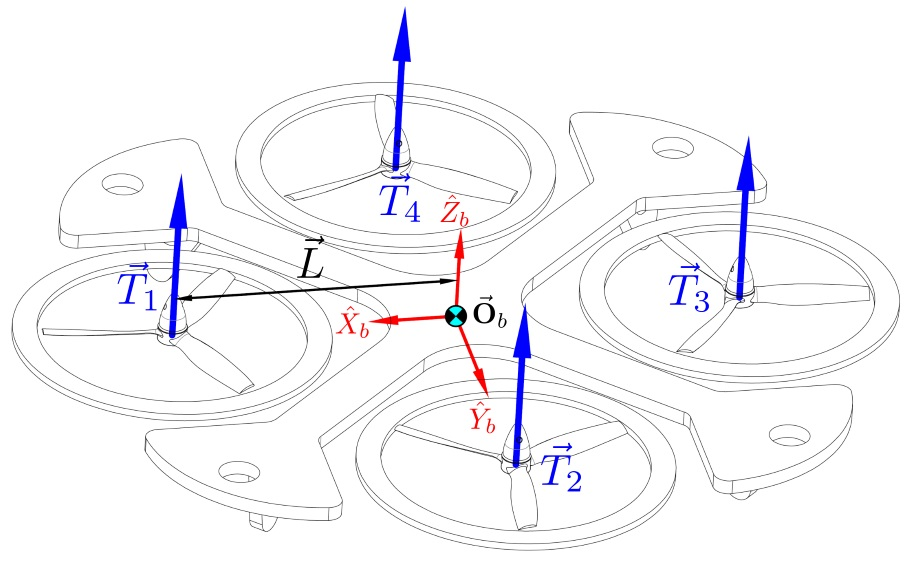
\includegraphics[width=0.8\textwidth]{figs/net-force}
\caption{Generalized quadrotor net forces and torques}
\label{fig:net-force}
\vspace{-14pt}
\end{figure}
\par
The net force $\vec{F}_\mu$ acting on the system is simply the sum of all thrust forces produced by rotating propellers, as some function of those rotational speeds; $\vec{T}(\Omega_i)$.
\begin{subequations}\label{eq:generalized-net-forces}
\begin{equation}
\vec{F}_\mu = \sum_{i=1}^4 \vec{T}(\Omega_i)~~~~[\text{N}],~\in\mathcal{F}^b
\end{equation}
Similarly net torque $\vec{\tau}_\mu$ is the sum of all \emph{differential} torque arms produced from opposing propeller thrust vectors. Each torque arm $\vec{L}_{1\rightarrow 4}$ is relative to the origin of \emph{motion} $\vec{\mathbf{O}}_b$.
\begin{equation}
\vec{\tau}_\mu = \sum_{i=1}^4 \vec{L}_i \times \vec{T}(\Omega_i)~~~~[\text{N.m}],~\in\mathcal{F}^{b}
\end{equation}
\end{subequations}
In Eq:\ref{eq:generalized-net-forces}, the thrust vector $\vec{T}(\Omega_i)$ is a function of the $i^{th}$ motor's rotational velocity $\Omega_i$, fixed in the $\hat{Z}_b$ direction. Each thrust vectors could potentially be $\in\mathbb{R}^3$. Similarly $\vec{l}_i$ is that thrust vector's perpendicular displacement from the origin $\mathbf{O}_b$. 
\par
The above equations are still applicable to any 6 DOF body, common simplifications applied to the system(s) for quadrotor control are explored in App:\ref{app:equations.standard}. Aerodynamic components pertinent for thrust and torque generation relative to Eq:\ref{eq:generalized-net-forces} are now introduced; obviously the contextual focus is on quadrotor and tilting quadrotor platforms\ldots
%====================================================
\section{Aerodynamics}
\label{sec:dynamics.aero}
%====================================================
The relationship between a propeller's rotational speed, $\Omega_i$ in $[\text{RPS}]$, and its perpendicular thrust vector, $\vec{T}(\Omega_i)$, is more complicated than the quadratic simplification taken at static conditions which most papers suggest (e.g \cite{x4flyer,modelingquadcopter} etc\ldots). The thrust produced is mostly dependent on the incident air stream flowing through the propeller's rotational plane; typically being the component of the body velocity normal to that propeller's plane. Fluid flowing \emph{tangentially} across the propeller's plane contributes toward in-plane aerodynamic drag (and hence torque). 
\par
The combination of aerodynamic blade-element\cite{bem,forwarddescent} and fluid-dynamics momentum (\emph{disc actuator}) theories equate an integral term generated across the propeller's length with the produced thrust or torque. A schedule of all aerodynamic effects encountered by a quadrotor's propellers is thoroughly detailed in both \cite{bladesforquadrotors} and \cite{nonlineardynamics}. The following is a review of pertinent aerodynamic theories; vortex ring state and parasitic drag effects are not included as they will be approximately negligible given the aircraft's proposed flight envelope with low translational velocities.
%====================================================
\subsection{Propeller Torque and Thrust}
\label{subsec:dynamics.aero.bem}
%====================================================
\emph{\color{Gray} A possible situation which the prototype could encounter is where an upstream propeller provides the incident fluid flow to another downstream propeller. Such a situation presents a complicated fluid dynamics and vortex wake effect problem. Propeller overlapping effects are discussed in \cite{configurationpropulsion} but remain open to further research in the context of the aircraft considered here.}
\par
To expedite the system identification process some simplifications are made on the aerodynamics to construct an approximate model; specifically using coefficients in place of complete local chord and pitch based integrals. Such an assumption holds true given that twisted, fixed pitch propellers are used (Fig:\ref{fig:fixed-pitch}) and not variable pitch swash-plate actuated propellers (Fig:\ref{fig:variable-pitch}).
\begin{figure}[htbp]
\centering
\begin{subfigure}{0.49\textwidth}
\centering
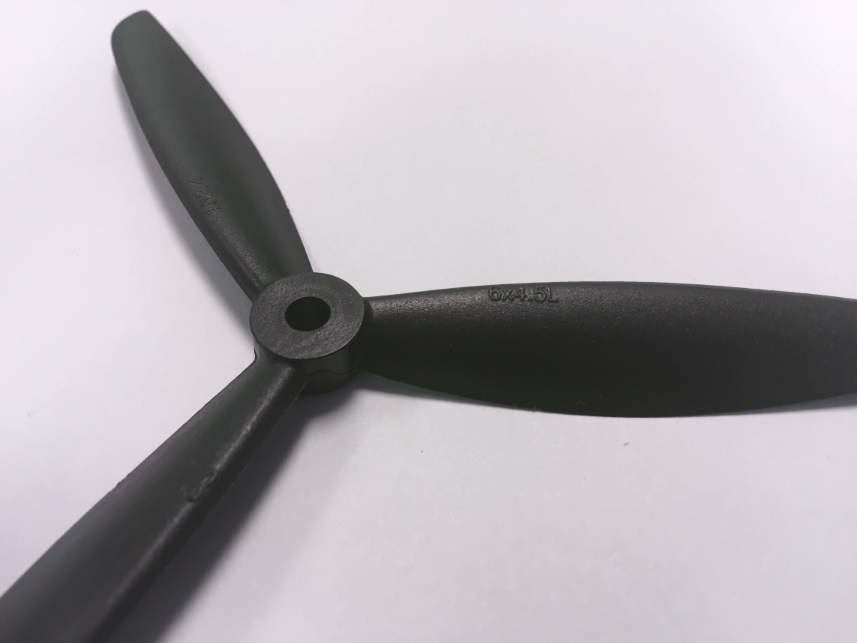
\includegraphics[width=0.8\textwidth]{figs/fixed-pitch}
\caption{Twisted, fixed pitch}
\label{fig:fixed-pitch}
\end{subfigure}
\begin{subfigure}{0.49\textwidth}
\centering
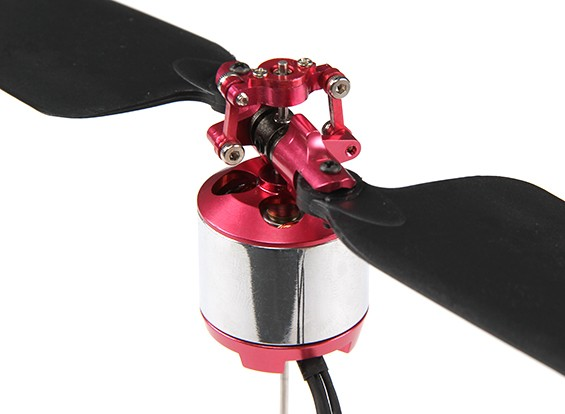
\includegraphics[width=0.8\textwidth]{figs/variable-pitch}
\caption{Swash-plate variable pitch; \cite{variablepitch}}
\label{fig:variable-pitch}
\end{subfigure}
\vspace{-6pt}
\caption{Propeller types}
\label{fig:props}
\vspace{-18pt}
\end{figure}
\par
A propeller's profile applies a perpendicular thrust force, $T$, onto the fluid in which it rotates. To build the following theoretical explanation propellers are first considered in terms of momentum theory; only perpendicular fluid flow through the propeller's plane is regarded. That fluid stream (Fig:\ref{fig:bem-flow}) has an incident upstream velocity, $v_\infty$, and a resultant slip velocity, $v_s$, downstream relative to the rotational plane. The change of fluid flow as a result of the propeller's rotation can be given as:
\begin{equation}
v_s = \Delta v + v_\infty
\end{equation}
Where $\Delta v$ is the net change in fluid velocity caused by the propeller blade's rotating aerofoil profile. The propeller induces a velocity directly in front of it's rotational plane, $v_i$, such that the net fluid flow into the plane is $v_b=v_i+v_\infty$. That induced inflowing fluid velocity is different to the net velocity contribution of the propeller; $v_i\not=\Delta v$.
\par
\begin{figure}[htbp]
\centering
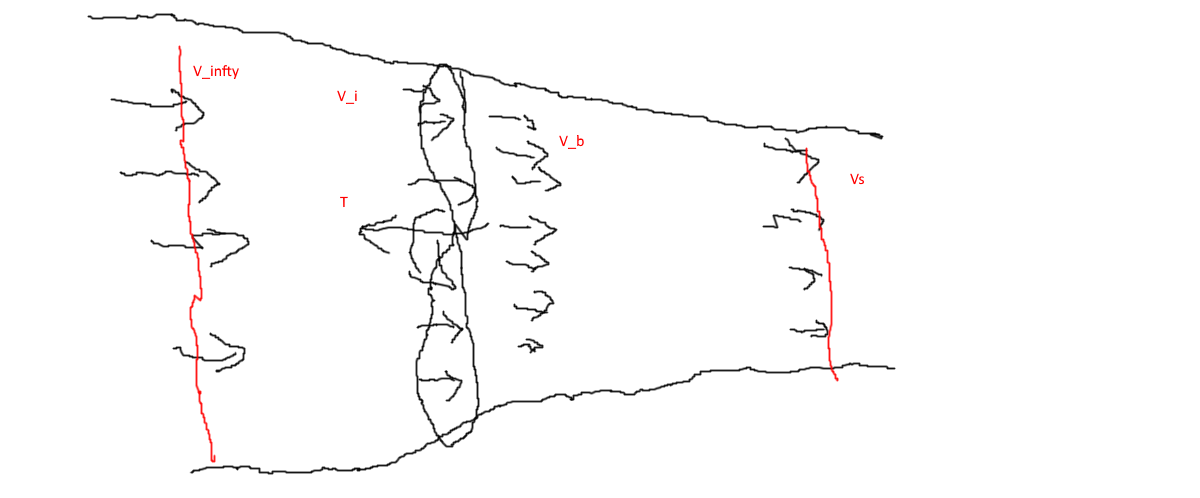
\includegraphics[width=0.6\textwidth]{figs/bem-flow}
\caption{Disc Actuator Propeller Planar Flow}
\label{fig:bem-flow}
\vspace{-15pt}
\end{figure}
It is shown in \cite{bladesforquadrotors} that, using Bernoulli's pressure theorem, the net fluid flow through the propeller's plane is:
\begin{equation}\label{eq:bernoulli}
v_b = \frac{1}{2} ( v_s - v_{\infty} ) = \frac{1}{2} \Delta v = \frac{1}{2} v_s \big|_{v_\infty=0}
\end{equation}
Stemming from classical disc actuator (fluid \emph{momentum}) theory, \cite{fluidmomentum}, the \underline{scalar} force $T(\Omega)$ acting on the fluid is calculated as a function of mass flow rate with respect to the change in fluid velocity (or \emph{pressure differential}):
\begin{equation}\label{eq:prop-mass}
T=(A_b v_b)\Delta v = \rho \pi R_b^2v_b \Delta v = \rho \pi R_b^2(v_i+v_\infty)\Delta v = \frac{1}{2} \rho \pi R_b^2 \Delta v^2
\end{equation}
Where $R_b$ is the disc (propeller) radius in $[\text{m}]$ for the fluid stream under consideration, $A_b$ is the area of that propeller disc. The fluid density of that stream, $\rho$, is typically $1.225~[\text{ kg.m}^{-3}]$ at standard temperature and pressure (\emph{stp}). However, the desired form of thrust generated is as a function of propeller rotational velocity $T(\Omega_i)$, so Eq:\ref{eq:prop-mass} is not satisfactory. 
\par
Eq:\ref{eq:prop-mass} can be solved as a function of aerodynamic propulsive power expended, $\Delta P=T\Delta v$. Rotational kinetic energy of a propeller and its transferred propulsive power is difficult to quantify, with compound parasitic losses deteriorating the efficiency of the propeller. Furthermore, the local fluid velocity through the propeller is not purely normal to the propeller plane but is in fact a vector. 
\par
In reality fluid flow induced by the propeller's rotation, $v_i$, directly in front of its plane of rotation is not purely perpendicular but has axial \underline{and} tangential induced components, termed $a$ and $a'$ respectively. Those induced components for the fluid velocity can be abstracted to induction factors dependent on the incident fluid velocity to the propeller's plane of rotation:
\begin{subequations}\label{eq:induction-factors}
\vspace{-5pt}
\begin{equation}\label{eq:induction-axial}
v_i=a v_\infty~~\text{in the axial direction}
\end{equation}
\vspace{-20pt}
\begin{equation}\label{eq:induction-tangential}
v_\theta=a' \Omega_i R_b~~\text{in the tangential direction}
\end{equation}
\end{subequations}
From induction factors defined Eq:\ref{eq:induction-factors}, the velocity components can be written as factors of upstream velocity $v_\infty$.
\begin{subequations}
\vspace{-5pt}
\begin{equation}
v_b=(1+a)v_\infty
\end{equation}
\vspace{-15pt}
\begin{equation}
v_s=(1+2a)v_\infty
\end{equation}
\end{subequations}
A consequence of the tangential fluid flow is that an angular momentum flow rate exists across the propeller plane. This produces a fluid-momentum torque opposing the rotational motion about the propeller's axis, analogous but perpendicular to Eq:\ref{eq:prop-mass}:
\begin{equation}\label{eq:prop-moment}
\vec{Q}=\rho\pi R_b^3 (v_\theta-v_\infty) v_b 
\end{equation}
\par
Together, Eq:\ref{eq:prop-mass} and Eq:\ref{eq:prop-moment} comprise propeller momentum theory but cannot be solved on their own. Blade-element theory analyses incremental aerofoil sections of width $dr$ of the propeller profile (the sectional view of which is illustrated in Fig:\ref{fig:bem-profile}) at some radius $r$. Each aerofoil element has a net local fluid velocity $\vec{U}$ across its profile, calculated as:
\begin{equation}
\vec{U}=\sqrt{(v_\infty+v_i)^2+(v_\Omega+v_\theta)^2}
\end{equation}
Where each profile has a chord length $c$ and an inclination (or \emph{pitch}) $\theta$ of the aerofoil \emph{zero-lift line} relative to the horizontal. Local fluid velocities incident to the propeller profile (shown in Fig:\ref{fig:bem-profile}) make their own angle of attack $\phi$ such that a true effective angle of attack $\alpha_{eff}$ is encountered:
\begin{equation}
\phi=\theta-\alpha_{eff}
\end{equation}
That local angle of attack varies with the incident fluid flow magnitude $v_\infty$ and the induced axial velocity $v_i$. That trigonometric ratio between the two is given as:
\begin{equation}
\phi=tan^{-1}\bigg(\frac{v_\infty+v_i}{v_\Omega+v_\theta}\bigg)=tan^{-1}\bigg(\frac{v_\infty(1+a)}{\Omega r(1+a')}\bigg)
\end{equation}
\par
\begin{figure}[hbtp]
\vspace{-15pt}
\centering
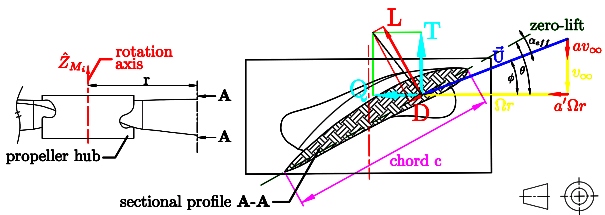
\includegraphics[width=\textwidth]{figs/bem-profile}
\caption{Blade element profile at radius r}
\label{fig:bem-profile}
\end{figure}
In-plane fluid flow $\vec{U}(r,\phi)$, for an element at radius $r$ with a local angle of attack $\phi$, then contributes towards elemental lift and drag forces as a function of aerofoil's dimensionless lift, $C_L$, and drag, $C_D$, coefficients. Those coefficients are determined by the aerofoil's characteristics, but would be constant across the length of a variable pitch, hinged and untwisted hinged prop (Fig:\ref{fig:variable-pitch}).
\begin{subequations}
\begin{equation}
\Delta L=\frac{1}{2}\rho \vec{U}(r,\phi)^2 c C_L
\end{equation}
\vspace{-10pt}
\begin{equation}
\Delta D=\frac{1}{2}\rho \vec{U}(r,\phi)^2 c C_D
\end{equation}
\end{subequations}
With air density $\rho$ typically taken at \emph{stp}. Lift and drag forces, when taken parallel and perpendicular to the plane of rotation, are thrust $T$ and torque $F_q$ forces (Fig:\ref{fig:bem-profile}). The in-plane force applies an aerodynamic torque $Q$ at the propellers hub because the force $F_q$ acts at a radius $r$, \cite{starmac}.
\begin{subequations}
\begin{equation}\label{eq:element-thrust}
dT=\frac{1}{2}\rho\vec{U}(r,\phi)^2c\big(C_L cos(\phi)+C_D sin(\phi)\big).dr
\end{equation}
\vspace{-5pt}
\begin{equation}\label{eq:element-drag}
dF_q=\frac{1}{2}\rho\vec{U}(r,\phi)^2c\big(C_L sin(\phi)+C_D cos(\phi)\big).dr
\end{equation}
\vspace{-5pt}
\begin{equation}\label{eq:element-torque}
\rightarrow dQ = \frac{1}{2}\rho\vec{U}(r,\phi)^2c\big(C_L sin(\phi)+C_D cos(\phi)\big)r.dr
\end{equation}
\vspace{-10pt}
\begin{equation}\label{eq:element-power}
\rightarrow dP = \Omega r dF_x .dr
\end{equation}
\end{subequations}
\par
Rotational power expended is a product of angular velocity and the opposing in-plane torque; Eq:\ref{eq:element-power}. Power is used in lieu of torque or drag terms in Eq:\ref{eq:element-torque} or Eq:\ref{eq:element-drag} respectively. Calculating forces and power terms as per momentum theory for each element, in terms of axial and tangential induction factors:
\begin{subequations}\label{eq:moment-thrust-element}
\begin{equation}
dT=\rho 4 \pi r^2 v_\infty(1+a)a.dr
\end{equation}
\vspace{-16pt}
\begin{equation}
dP=\rho 4 \pi r^2 v_\infty(1+a)\Omega r (1+a').dr
\end{equation}
\end{subequations}
Equating momentum and element terms produces the blade-element momentum equation(s) for aerodynamic thrust and power from a propeller. Following a few assumptions; most importantly that the lift coefficient $C_L$ is a linear function of the effective angle of attack $\alpha_{eff}$. 
\begin{equation}
C_L=a_L(\theta-\phi)
\end{equation}
Firstly the lift coefficient curve gradient $a_L$ is shown in \cite{aerodynamicsforengineering} for an ideally twisted blade, like the fixed pitch propellers under consideration here, to be $2\pi$. An ideal lift coefficient is then a function:
\begin{equation}\label{eq:lift-curve-gradient}
C_L=2\pi(\theta-\phi)
\end{equation}
Secondly assuming tangentially induced velocities, $v_\theta$, are small when compared to the propeller's speed translational speed at radius $r$, $v(r)=\Omega r$. The tangential induction factor $a'$ is then:
\begin{equation}
a'=\frac{v_\theta}{\Omega r}<<1
\end{equation}
Small angle approximations then apply to Eq:\ref{eq:element-thrust}-\ref{eq:element-torque}; $cos(\phi+\alpha_{eff})\approx 1$ and $sin(\phi+\alpha_{eff})\approx \phi+\alpha_{eff}$. Similarly net inflow and axial velocities are $v_\infty + v_i<<\Omega r$, the following integrals are then found:
\begin{subequations}
\begin{equation}\label{eq:bem-thrust}
T=\int_{r=0}^R \frac{1}{2} a_L b c \rho (\Omega r)^2 \bigg[\theta-\frac{v_\infty+v_i}{\Omega r}\bigg].dr
\end{equation}
\begin{equation}\label{eq:bem-power}
P=\int_{r=0}^R \frac{1}{2}a_L b c \rho (\Omega r)^3\bigg[\big(\theta-\frac{v_\infty+v_i}{\Omega r}\big)\big(\frac{v_\infty+v_i}{\Omega r}\big) + C_d\bigg].dr
\end{equation}
\end{subequations}
Where $b$ is the number of blades the propeller has. In practice knowing exact pitch and chord values as a function of $r/R$ is difficult and calculating integrals at each process step is cumbersome. Both Eq:\ref{eq:bem-thrust} and Eq:\ref{eq:bem-power} can be solved by equating element and momentum terms (a full expansion is given in Appendix:\ref{app:equations.bem}). Often dimensionless thrust, torque and power coefficients are defined across the entire blade's length:
\begin{subequations}\label{eq:coefficients}
\begin{equation}\label{eq:thrust-coefficient}
C_T(J)=\frac{T}{\rho \Omega^2 D^4}
\end{equation}
\vspace{-6pt}
\begin{equation}\label{eq:power-coefficient}
C_P(J)=\frac{P}{\rho \Omega^3 D^5}
\end{equation}
\end{subequations}
Where $\Omega$ is the propeller's rotational speed in \underline{revolutions per second} (\emph{RPS}) and different from other inertial equations like Eq:\ref{eq:angular-rot}, with units $[\text{rad.s}^{-1}]$. The propeller diamater $D$ is in $[\text{m}]$. For fixed pitch propellers the thrust and power coefficients are easily determined and remain consistent. Both Eq:\ref{eq:thrust-coefficient} and Eq:\ref{eq:power-coefficient} vary as a function of the dimensionless \emph{advance ratio} $J$.
\begin{equation}\label{eq:advance}
J = \frac{v_\infty}{\Omega R}
\end{equation}
Typically the net upstream velocity $v_\infty$ is simply the perpendicular component (projected onto the plane's normal vector $\hat{n}$, Eq:\ref{eq:normal-fluid}) of the vehicle's translational velocity in the body frame, $\vec{v}_b\perp\hat{n}$. For the case of a zero advance ratio, $J=0$, the conditions are regarded as static. Static thrust and power coefficients are nominal in their values.
\par
Propeller databases like \cite{UIUC} provide comprehensive coefficient values for a range of small and medium diameter propeller types at different advance ratios. Included in the database are blade profiles, pitch and chord lengths; all the results are outcomes of the investigation \cite{lowreynolds}. 
\par
The introduction of those coefficients drastically reduces the thrust estimation process. For a typical $6\times 4.5$ inch propeller, the coefficients used were linearly interpolated from similar pitched database results from \cite{UIUC} to match subsequent physical test values. The static thrust and power coefficients are respectively:
\begin{subequations}
\begin{equation}
{\color{blue}C_{T0}}=0.191
\end{equation}
\vspace{-15pt}
\begin{equation}
{\color{red}C_{P0}}=0.0877
\end{equation}
\end{subequations}
Fig:\ref{fig:coeffs-plot} shows plots coefficients for thrust, {$\color{Blue}C_{T}$}, and power, {$\color{Red}C_{P}$}, as a function of the advance ratio $J$. As the incident upstream fluid velocity, $v_\infty$, increases, the thrust coefficient decreases. So too does the power coefficient and hence the aerodynamic torque. The thrust and power coefficients can be assumed constant for low advance ratios, or in the case considered here, translational velocities.
\begin{figure}[htpb]
\vspace{-12pt}
\centering
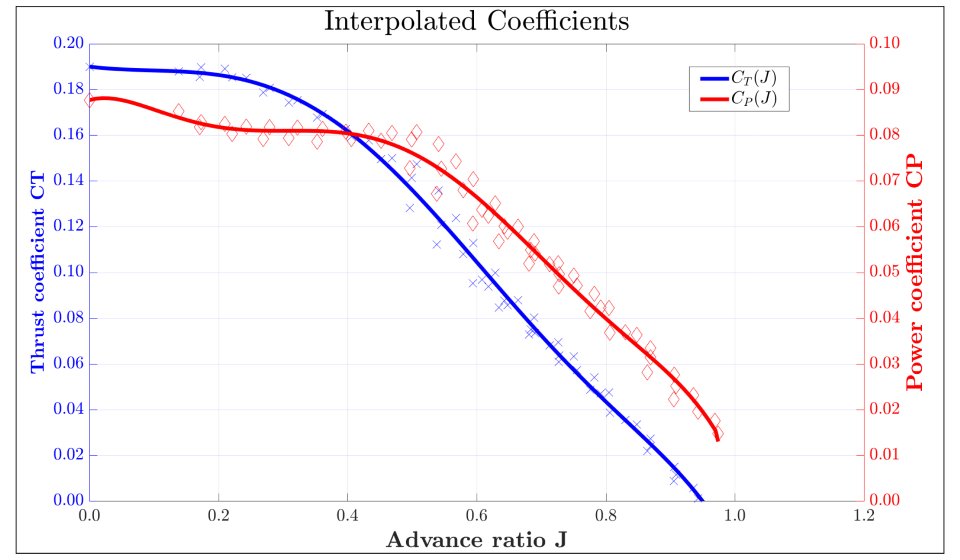
\includegraphics[width=0.7\textwidth]{graphs/coeffs-plot}
\vspace{-12pt}
\caption{Power \& thrust coefficients}
\vspace{-16pt}
\label{fig:coeffs-plot}
\end{figure}
\par
Plotted in Fig:\ref{fig:thrusts} and Fig:\ref{fig:torques}, both thrust and torque test rigs and their static test results are illustrated. Measured values for each test are plotted; {\color{Red}$T(\Omega)$} in Fig:\ref{fig:thrust-plot} for thrust and {\color{Red}$Q(\Omega)$} in Fig:\ref{fig:torque-plot} for torque. The physically tested values are fitted with quadratic trend-lines and plotted against static coefficient estimates using Eq:\ref{eq:thrust-coefficient} for thrust {\color{LimeGreen}$\hat{T}C_t(\Omega)$} and Eq:\ref{eq:power-coefficient} for calculated torque {\color{LimeGreen}$\hat{Q}C_p(\Omega)$}. Results from Fig:\ref{fig:coeffs-plot} are used as a lookup table and values from Eq:\ref{eq:coefficients} are calculated, induced propeller thrust and torques can be accurately modeled quadratically, the power term is cubic with respect to its rotational velocity. 
\begin{figure}[htbp]
\centering
\begin{subfigure}{0.49\textwidth}
\centering
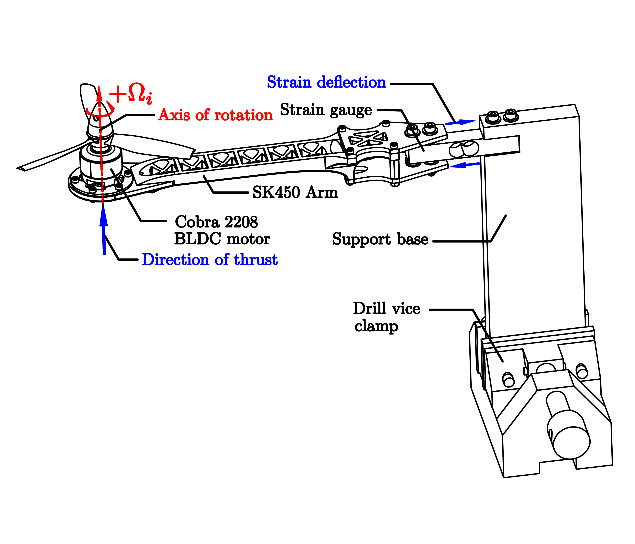
\includegraphics[width=\textwidth]{figs/thrust-rig}
\vspace{-20pt}
\caption{Thrust deflection test rig}
\label{fig:thrust-rig}
\end{subfigure}
\begin{subfigure}{0.49\textwidth}
\centering
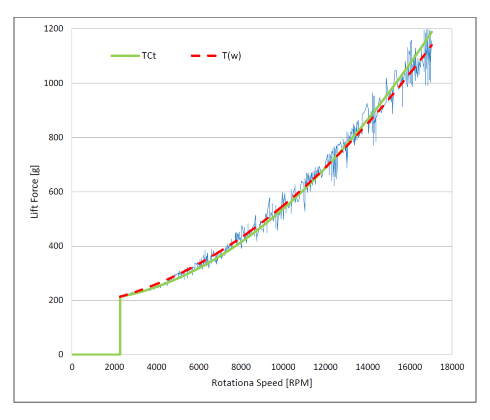
\includegraphics[width=\textwidth]{graphs/thrust-plot}
\vspace{-20pt}
\caption{Static thrust plot}
\label{fig:thrust-plot}
\end{subfigure}
\vspace{-8pt}
\caption{Propeller thrust tests}
\label{fig:thrusts}
\end{figure}
\par
\begin{figure}[hbtp]
\begin{subfigure}{0.5\textwidth}
\centering
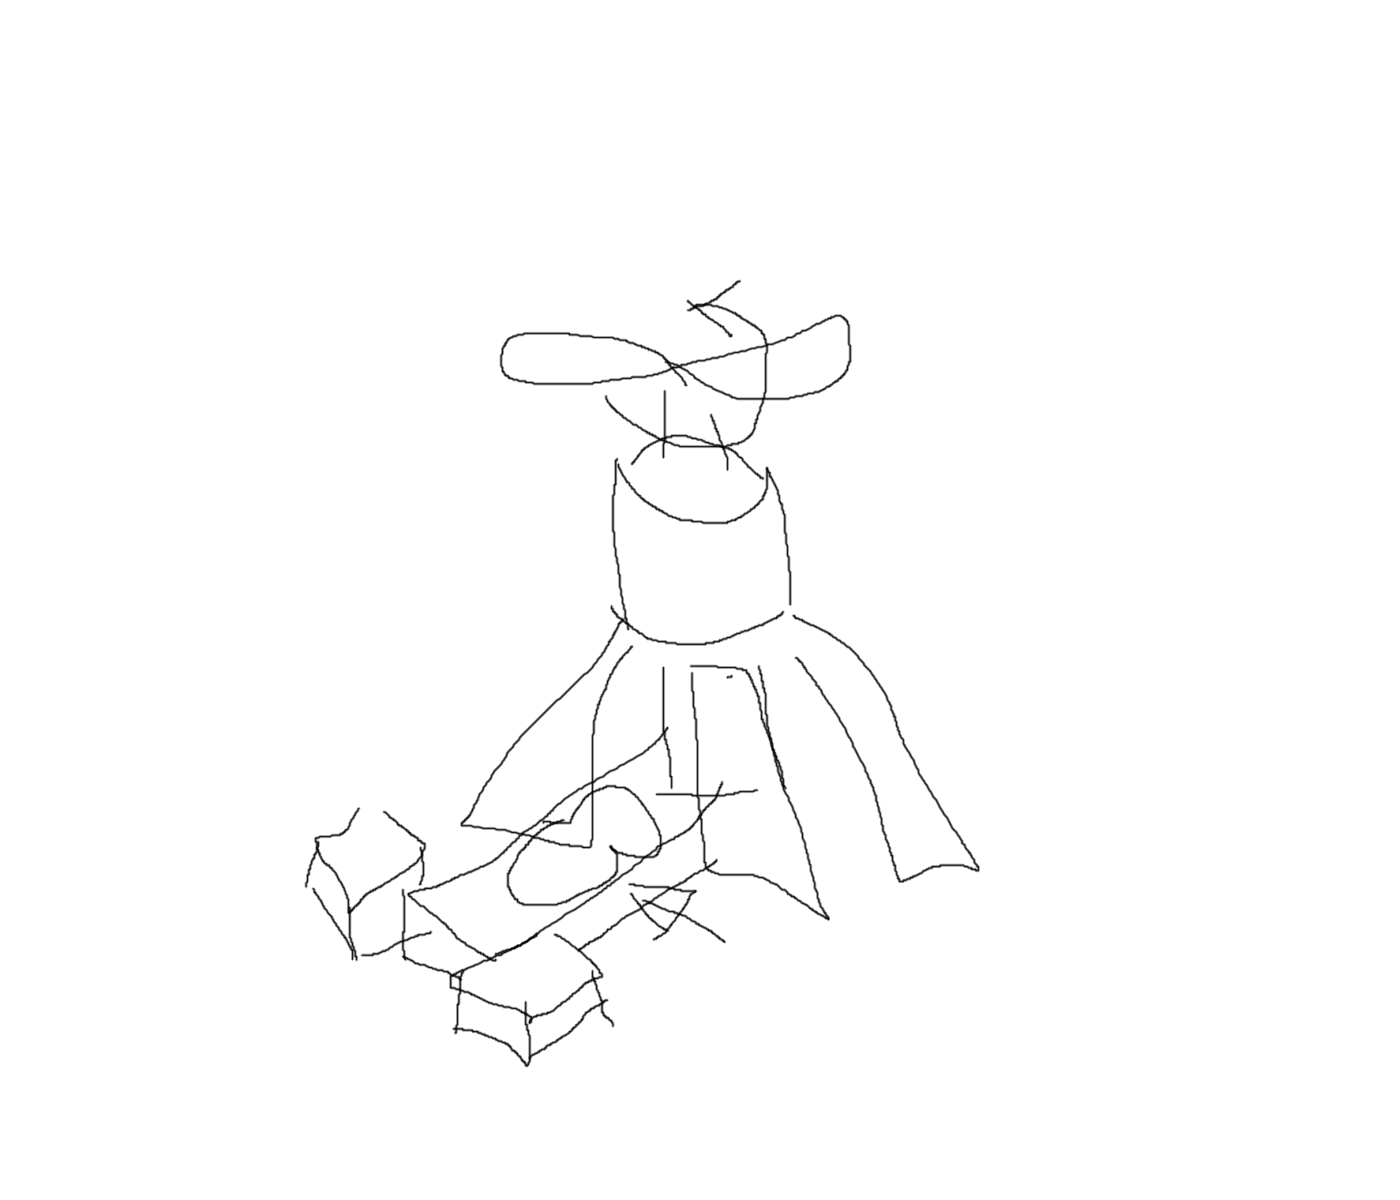
\includegraphics[width=\textwidth]{figs/torque-rig}
\vspace{-20pt}
\caption{Torque test rig}
\label{fig:torque-rig}
\end{subfigure}
\begin{subfigure}{0.5\textwidth}
\centering
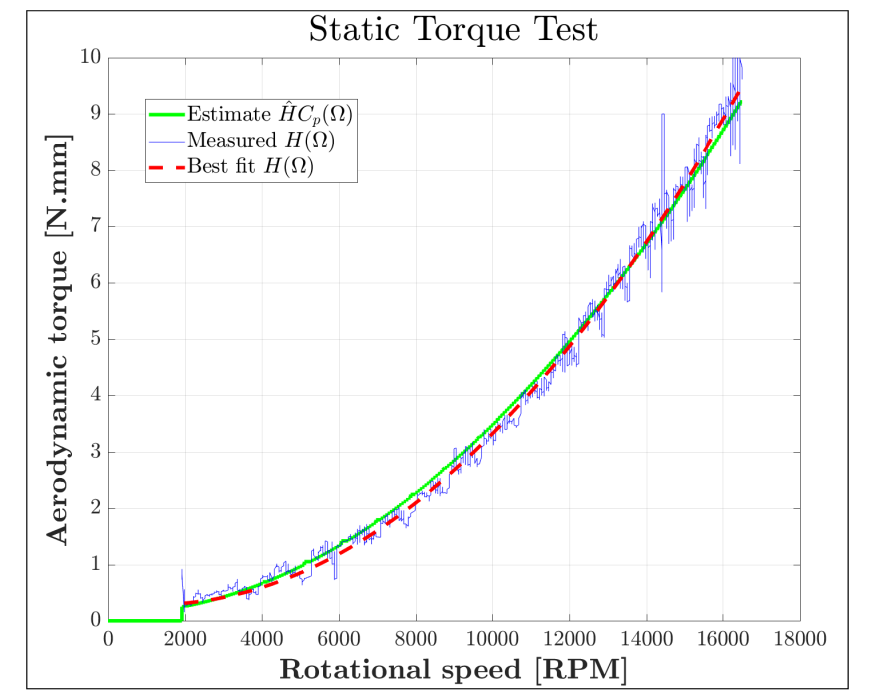
\includegraphics[width=\textwidth]{graphs/torque-plot}
\vspace{-20pt}
\caption{Torque plot}
\label{fig:torque-plot}
\end{subfigure}
\caption{Static torque tests}
\label{fig:torques}
\vspace{-8pt}
\end{figure}
Advance ratios, or rather the propeller incident fluid flow(s), are dependent on the vehicle's net translational and angular velocity. Such that the fluid velocity's normal component to the propeller plane is given by:
\begin{equation}\label{eq:normal-fluid}
v_\infty = (\vec{v}_b + \vec{L}_{arm}\times \vec{\omega}_b)\cdot \hat{n}~~~~\in\mathcal{F}^{M_i}
\end{equation}
Where $\vec{v}_b~~[\text{m.s}^{-1}]$ is the body's transnational velocity and $\vec{\omega}_b~~[\text{rad.s}^{-1}]$ is the body's angular velocity, both transformed to the propeller's frame, $\in\mathcal{F}^{M_i}$. Furthermore $\hat{n}(\lambda_i,\alpha_i)$ is the unit vector normal to the propeller's rotational plane, relative to the body velocity. Then $J$ is calculated from Eq:\ref{eq:advance}.
\par
{\color{Gray}\emph{It's worth reiterating that the above static coefficients are indeed calculated from physical static tests. However advance ratio coefficient dependencies are linearly interpolated from the closest available matching data (APC Thin-Electric 8X6 propellers) cited from \cite{UIUC}}.}
\par
Clockwise and counterclockwise propellers and rotations were used for both thrust and torque tests. Despite the thrust and test rigs having been designed to isolate each respective response, results from opposing directional tests were averaged in the hopes that unwanted opposing effects were negated. Both positive and negative rotational test results for thrust and torque measurements are included in Appendix:\ref{app:thrust-torque}
\par
{\color{Gray}\emph{Discrepancies which emerge between the model or coefficient values derived can be accounted for with lumped uncertainty disturbance term(s). Model uncertainty compensation can easily be incorporated into adaptive backstepping or $H_\infty$ control algorithms. The deviation of the modeled thrust or torques from their true values would be simple to incorporate into a plant dependent Lyapunov candidate function; Sec:\ref{subsubsec:control.attitude.nonlinear.adaptivebackstep}.}}
%====================================================
\subsection{Hinged Propeller Conning \& Flapping}
\label{subsec:dynamics.aero.flap}
%====================================================
Other non-linear effects which adversly effect a propeller's performance have all been well documented in their own right in the context of helicopter aerodynamic and propeller fields\cite{basichelicopter,bramwell}. Typically such effects are more pronounced when observing hinged variable pitch propellers, fixed pitch propellers have a diminished effect. Moreover, low translational velocities suppress such responses but they're worth mentioning.
\par
Conning and flapping are the two most significant aerodynamic effects encountered by a propeller. Other phenomenon like cyclic vortex ring states are deemed to not be applicable here and fall outside the scope of the investigation. 
\par
In translational flight, for a propeller without shrouding or a ducting, each blade encounters varying incident fluid flow throughout its cycle. The advancing blade relative to the body's translational direction encounters a greater fluid flow than the retreating blade, constructive and destructive interference from the body's translational velocity adds to local fluid flows. The effective local angle(s) of attack for the opposing advancing and retreating propeller blades are not symmetrical from such variations. Those unbalanced angles of attack produce a dissymmetry of lift across the propeller blade's surface.
\par
\begin{figure}[htbp]
\centering
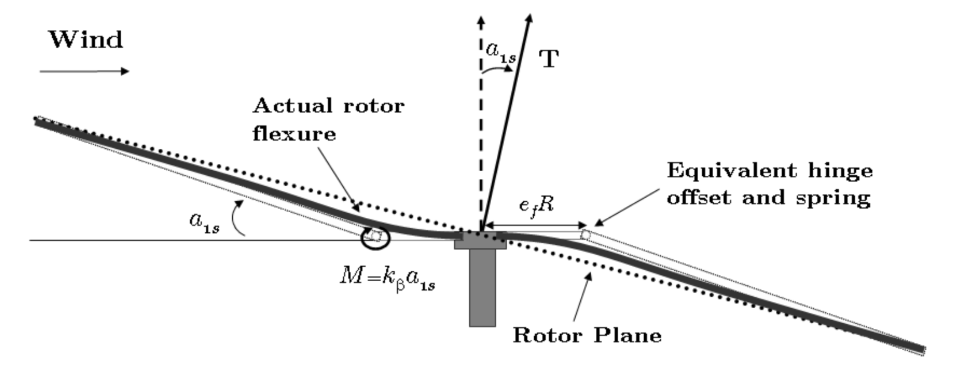
\includegraphics[width=\textwidth]{figs/prop-flap}
\caption{Propeller blade flapping; from \cite{starmac}}
\label{fig:prop-flap}
\end{figure}
\par
Throughout each rotation the blade is forced up and down as it cycles through a varying fluid velocity field, applying a torque moment about the propeller's hub. That torque's magnitude is a function of the body's net translational velocity and the propeller material's stiffness (hence its susceptibility to deflection). The flapping pitches the effective propeller plane (\emph{tip-path plane}), and hence the thrust vector line, away from its principle axis (Fig:\ref{fig:prop-flap}).
\par
The propeller's resultant thrust vector is pitched away from its nominal perpendicular state by some deflection angle, $\alpha_{1s}$ in Fig:\ref{fig:prop-flap}, toward the direction of translational movement or wind disturbance. Propeller flapping is diminished at low translational velocities with small wind disturbances relative to propeller rotational speed. As such flapping is not applicable to the feasible flight envelope envisaged for the prototype here.
\par
\begin{figure}[hbtp]
\centering
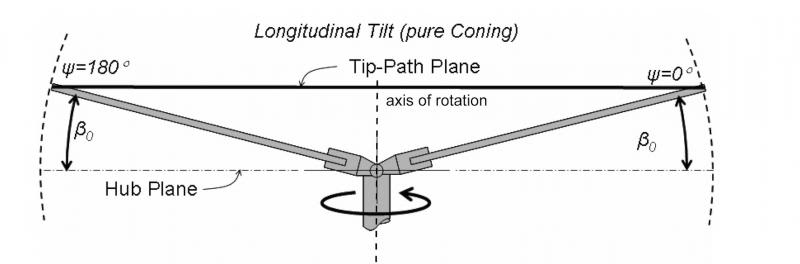
\includegraphics[width=0.95\textwidth]{figs/prop-coning}
\caption{Propeller coning}
\label{fig:prop-coning}
\end{figure}
Coning (illustrated in Fig:\ref{fig:prop-coning}) is another form of propeller deflection, which again is dependent on the blade material's stiffness. Coning causes both advancing and retreating propeller blades to both deflect upward. Distributed loading on the propeller surface from supporting a body's weight causes the upward deflection. The coning reduces the effective propeller disc's radius, adversely affecting thrust produced, Eq:\ref{eq:bem-thrust}. Increased loading accentuates the coning angle experienced by the propellers and as such reduces the tip-path-plane.
\par
Both aerodynamic induced propeller deflection effects can be quantified numerically. Their derivation and resultant equations are cumbersome however. In due course both effects on the produced prototype are not significant enough to produce instability if neglected. The frame could potentially be affected in more adverse ways given certain flight conditions with higher translational velocities or incident wind and fluid flow disturbances\ldots
%====================================================
\subsection{Drag}
\label{subsec:dynamics.aero.drag}
%====================================================
For any solid body with some non-zero relative translational velocity motion within a fluid, there is a second order damping response opposing translational velocity. The net drag force, $\vec{D}_{net}$, although locally dependent on individual component cross-sections can be abstracted to a drag coefficient matrix representing the whole body. For a velocity $\vec{v}$:
\begin{equation}
\vec{v}=\begin{bmatrix}
u\\
v\\
w
\end{bmatrix}~~~~[\text{m.s}^{\text{-}1}]\in\mathcal{F}^{b}
\end{equation}
The drag equation is given by:
\begin{equation}\label{eq:distrubance}
\vec{D}_{net}(\vec{v})=\begin{bmatrix}
D_{ii} & D_{ij} & D_{ik}\\
D_{ji} & D_{jj} & D_{jk}\\
D_{ki} & D_{kj} & C_{kk}
\end{bmatrix}
\begin{bmatrix}
u\\
v\\
w
\end{bmatrix}^2
~~~~[\text{N}],~\in\mathcal{F}^b
\end{equation}
Each drag coefficient's subscript; $\hat{i},\hat{j}$ and $\hat{k}$ are dependent on the frame's directional cross-section area for each $\hat{X}_b,\hat{Y}_b,\hat{Z}_b$ axis respectively. Given a well designed and symmetrical frame, it can be assumed the off-diagonal elements are of little or no consequence and as such the drag equation can be simplified to a diagonal form:
\begin{equation}
\vec{D}_{net}(\vec{v})\approx diag\big(D_{ii},~D_{jj},~D_{kk}\big)\vec{v}^{\hspace{2pt}2}~~~~\in\mathcal{F}^b
\end{equation}
Given the second order dependency on translational velocity of the opposing drag forces, such terms can be relegated to a lumped disturbance terms to be adaptively compensated for in the control loop, Sec:\ref{subsubsec:control.attitude.nonlinear.adaptivebackstep}. The time scale separation between velocity and wind drag effects with the control loop allow for such an assumption. Analogous drag-like effects opposing angular rotation rates exist but, for the intents and purposes of most practical flight envelopes, can be disregarded.
\par
In simulation; if the plant has sufficient disturbance rejection then the drag term in Eq:\ref{eq:distrubance} would be easily accounted for an adaptive backstepping algorithm. Furthermore it is possible to physically test for the drag coefficients to attain a higher certainty model but, given the flight conditions for this research, such effects will be small if not negligible. As such those tests are outside the scope of investigation here\ldots
%====================================================
\subsection{Rotation Matrix Singularity}\label{subsec:dynamics.rigidbody.singularity}
%====================================================
The singularity inherent to Euler Angle parametrization is often mentioned but far less common is the mathematical demonstration of how that singularity manifests itself.  A singularity occurs for some matrix $A$ in $\vec{y}=A\vec{x}$ when the matrix has a zero determinate; losing rank and differentiability in terms of $\vec{x}$. The combined rotation matrix from the $\mathcal{F}^{I}$ to $\mathcal{F}^{b}$ is the singular component of an Euler parametrized sequence. Considering the case of a rotational 3-axis gimbal system (Fig:\ref{fig:gimbal}) which mimics the sequential nature of the Euler set. When the intermediary sequenced rotational angle is at $\pi/2$, the remaining two axes become co-linear (Fig:\ref{fig:gimbal-lock}). In Z-Y-X rotation sequence adopted in this work, the singularity occurs from the rolling angle $\theta$ about $\hat{Y}$. Both the pitch $\phi$ or yaw $\psi$ rotations will subsequently have the same rotational effect. Such a situation results in as a loss of a degree of freedom.
\begin{figure}[htbp]
\begin{subfigure}{0.5\textwidth}
\centering
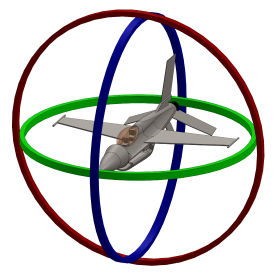
\includegraphics[width=0.9\textwidth]{figs/gimbal}
\caption{3-Axis gimbal}
\label{fig:gimbal}
\end{subfigure}
\begin{subfigure}{0.5\textwidth}
\centering
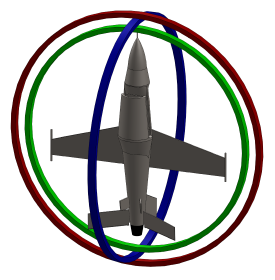
\includegraphics[width=0.9\textwidth]{figs/gimbal-lock}
\caption{Locked gimbal with loss of DOF}
\label{fig:gimbal-lock}
\end{subfigure}
\caption{Mechanical gimbal lock}
\vspace{-15pt}
\end{figure} 
\par
What is clear physically is not necessarily as obvious mathematically. A loss of rank occurs in the Euler Matrix $\Psi(\eta)$, defined previously in Eq:\ref{eq:angular-rates.e} from Sec:\ref{subsec:proto.conventions.frames}. That relation between angular velocity, in the inertial frame or inversely in the body frame, and the angular rates of the Euler Angles has a determinant:
\begin{equation}\label{eq:euler-derivative}
\begin{bmatrix}
\dot{\phi}\\
\dot{\theta}\\
\dot{\psi}
\end{bmatrix}
=\begin{bmatrix}
1 & sin(\phi)tan(\theta) & cos(\phi)tan(\theta)\\
0 & cos(\phi) & -sin(\phi)\\
0 & sin(\phi)sec(\theta) & cos(\phi)sec(\theta)\\
\end{bmatrix}
\begin{bmatrix}
p\\
q\\
r
\end{bmatrix}
=\Phi(\eta)\omega_b
\end{equation}
\vspace{-2pt}
\begin{equation}
\rightarrow det\big(\Phi(\eta)\big)=cos(\phi)\big(cos(\phi)sec(\theta)\big)+sin(\phi)\big(\sin(\phi)sec(\theta)\big)=sec(\theta)
\end{equation}
\vspace{-6pt}
\begin{equation}
\therefore \underset{{\theta \rightarrow \pi /2}}{lim}|\Phi(\eta)|=sec(\theta)\rightarrow \infty
\end{equation}
The Euler matrix $\Phi(\eta)$ looses rank as $\theta\rightarrow\pi/2$, loosing differentiability as well. The physical consequence of this is the loss of a degree of freedom. More specifically, if one looks at how the Z-Y-X rotation (or transformation) matrices are formulated, from Eq:\ref{eq:rotationmatrix}.
\begin{subequations}
\begin{equation}
R_I^b(\eta)= R_z(\psi)R_y(\theta)R_x(\phi)=\begin{bmatrix}
c_\psi & -s_\psi & 0\\
s_\psi & c_\psi & 0\\
0 & 0 & 1
\end{bmatrix}
\begin{bmatrix}
c_\theta & 0 & s_\theta\\
0 & 1 & 0\\
-s_\theta & 0 & c_\theta
\end{bmatrix}
\begin{bmatrix}
1 & 0 & 0\\
0 & c_\phi & -s_\phi\\
0 & s_\phi & c_\phi
\end{bmatrix}
\end{equation}
\begin{equation}
\therefore R_I^b(\eta)=\begin{bmatrix}
c_\psi c_\theta & c_\psi s_\theta s_\phi - s_\psi c_\phi & c_\psi s_\theta c_\phi + s_\psi s_\phi\\
s_\psi c_\theta & s_\psi s_\theta s_\phi + c_\psi c_\phi & s_\psi s_\theta  c_\phi - c_\psi s_\phi\\
-s_\theta & c_\theta s_\phi & c_\phi c_\theta\\
\end{bmatrix}
\end{equation}
In the case where $\theta=\pi/2$, and using trigonometric double angles, the following can be reduced;
\begin{equation}
R_I^b(\eta)=\begin{bmatrix}
0 & c_\psi s_\phi - s_\psi c_\phi & c_\psi c_\phi + s_\psi s_\phi\\
0 & s_\psi s_\phi + c_\psi c_\phi & s_\psi c_\phi - c_\psi s_\phi\\
-1 & 0 & 0\\
\end{bmatrix}\Bigg|_{\theta=\pi/2}
\end{equation}
\vspace{-6pt}
\begin{equation}
=
\begin{bmatrix}
0 & s(\phi - \psi) & c(\phi - \psi)\\
0 & c(\phi - \psi) & s(\phi - \psi)\\
-1 & 0 & 0
\end{bmatrix}
\end{equation}
\vspace{-4pt}
\begin{equation}\label{eq:gimbal}
=R_{x'}(\phi-\psi)
\end{equation}
\end{subequations}
Where the resultant in Eq:\ref{eq:gimbal} represents an $\hat{X}'$-axis rotation in a new intermediate frame, post a $\pi/2$ rotation about the $\hat{Y}$-axis. Through trigonometric double angles a degree of freedom is lost at $\theta=\pi/2$, when $\phi$ \& $\psi$ effect the same angle.
%====================================================
\subsection{Quaternion Dynamics}
\label{subsec:dynamics.rigidbody.quaternion}
%====================================================
An algorithm proposed in \cite{euleranglesingularity} suggested a solution to avoid Euler Angle singularities. The heuristic proposed involved switching between sequence conventions (ZYX,ZYZ etc\ldots there are 12 in total) such that the singularity is always avoided. However the implementation of such an algorithm is cumbersome and inefficient. Far more elegant is the use of \emph{quaternion} attitude representations in $\mathbb{R}^4$ (in \cite{rotationsequences,quaterniondynamics,spacecraftattitutdequaternions} amongst others\ldots most notably made popular by \cite{shoemake} for use in animation).
\par
A quaternion is analogous to a rotation matrix in that it represents an attitude difference between two reference frames. An $\mathbb{R}^3$ attitude is paramterized as one rotation $\theta$ about a single unit \emph{Euler} axis $\hat{u}$ (demonstrated using the Rodriguez Formula in \cite{unwinding}). In brief a quaternion consists of a scalar component, $q_0$, and complex vector component, $\vec{q}\in \mathbb{C}^3$, such that:
\begin{equation}
Q\triangleq 
\begin{bmatrix}
q_0 \\
\vec{q}
\end{bmatrix}
~~\in\mathbb{R}^4
\end{equation}
The relationship between an Euler Angles rotation matrix $R_I^b(\eta)$ and a quaternion attitude $Q_b$ is given by the Rodriguez formula:
\begin{equation}\label{eq:rodriguez}
R_I^b(\eta)=R(Q_b)=\mathbb{I}_{3\times 3}+2q_0[\vec{q}\hspace{2pt}]_\times+2[\vec{q}\hspace{2pt}]_\times\text{}^2
\end{equation}
Where $[.]_\times$ is the cross-product matrix defined earlier in Eq:\ref{eq:cross-product-matrix}. All quaternions, unless otherwise specified, are unit quaternions $Q\in\mathbb{Q}_u$. Quaternion with a unity magnitude ensure that rotational operations maintain the vector operand's magnitude. A unit quaternion is defined:
\begin{equation}
\norm{Q}=\sqrt{{q_0}^2+\vec{q}\text{}\hspace{2pt}^2}=1
\end{equation}
Quaternion multiplication is distributive and associative, but not commutative. Specifically a quaternion multiplciation operation is equivalent to the Hamilton product. For two quaternions, $Q$ \& $P$:
\begin{subequations}
\begin{equation}
Q\otimes P = \begin{bmatrix}
q_0 \\
\vec{q}
\end{bmatrix}
\otimes
\begin{bmatrix}
p_0 \\
\vec{p}
\end{bmatrix}
\end{equation}
\begin{equation}
\triangleq\begin{bmatrix}
q_0p_0-\vec{q}\cdot\vec{p}\\
q_0\vec{p}+p_0\vec{q}+\vec{q}\times\vec{p}
\end{bmatrix}
\end{equation}
\begin{equation}\label{eq:quaternion-product}
=q_0 p_0 - \vec{q}\cdot \vec{p}+p_0 \vec{q} + q_0 \vec{p} + \vec{q}\times\vec{p}
\end{equation}
\end{subequations}
Because the vector component of a quaternion is complex valued, it is natural that there exists a quaternion complex conjugate property, defined as:
\begin{equation}
Q^*=\begin{bmatrix}
q_0 \\
-\vec{q}~
\end{bmatrix}
\end{equation}
It then follows that the fundamental quaternion identity is:
\begin{equation}
Q\otimes Q^* = \mathbb{I}_{4\times 4}
\end{equation}
A right handed quaternion rotation applied to a vector $\vec{\nu} \in\mathbb{R}^3$ involves multiplication by two unit quaternions. 
\begin{equation}
\begin{bmatrix}
0 \\
\vec{\nu}\hspace{2pt}'
\end{bmatrix}
=Q\otimes
\begin{bmatrix}
0 \\
\vec{\nu}
\end{bmatrix}
\otimes Q^*
\end{equation}
Mostly, the zero scalar components are omitted in a rotation (\emph{or transformation}) operation, it is implied that vector operands are substituted with quaternions.
\begin{equation}\label{eq:quaternion-rotation}
\vec{\nu}\hspace{2pt}'=Q \otimes (\vec{\nu}\hspace{2pt}) \otimes Q^*
\end{equation} 
In the case of rigid body attitude parameterization with quaternions, $Q_b$ is the quaternion which represents the difference between $\mathcal{F}^b$ and $\mathcal{F}^I$. A quaternion operator is equivalent to a rotation matrix operation, for some vector $\vec{\nu}_I\in\mathcal{F}^I$;
\begin{equation}
\vec{\nu}_b=R_I^b(\eta)\vec{\nu}_I \underset{Q}{\iff} Q_b \otimes (\vec{\nu}_I) \otimes Q_b^*
\end{equation}
Since quaternions are non-commutative, the construction of a body quaternion $Q_b$ from an Euler angle set $\vec{\eta}$ is sequence dependent. Euler angles, despite being singular, are conceptually simple terms for describing a body's orientation. A Z-Y-X sequenced body quaternion, $Q_b$, can be constructed from Euler angles as:
\begin{equation}\label{eq:quaternion-sequence}
Q_b=Q_z\otimes Q_y\otimes Qx=\begin{bmatrix}
cos(\psi/2)\\
0\\
0\\
sin(\psi/2)
\end{bmatrix}
\otimes
\begin{bmatrix}
cos(\theta/2)\\
0\\
sin(\theta/2)\\
0
\end{bmatrix}
\otimes
\begin{bmatrix}
cos(\phi/2)\\
sin(\phi/2)\\
0\\
0
\end{bmatrix}
\end{equation}
A quaternion's time derivative, defined in \cite{quaterniondynamics}, with $Q_\omega$ being a quaternion with a vector component equal to angular velocity $\vec{\omega}_{b/I}$ and a zero scalar component, is:
\begin{equation}\label{eq:quaternion-deriv}
\frac{d}{dt}Q_b=\frac{1}{2}Q_b\otimes Q_{\omega}=\begin{bmatrix}
-\frac{1}{2}\vec{q}\hspace{2pt}^{T} \vec{\omega}_b\\
\frac{1}{2}\big([\vec{q}\hspace{2pt}]_\times+q_0\mathbb{I}\big)\vec{\omega}_b
\end{bmatrix}
\end{equation}
Using quaternions to represent attitudes negates the need for an Euler Matrix, $\Phi(\eta)$, to represent attitudes and their rates. A body quaternion is fully defined in the inertial frame with respect to the body frame or inversely so. The first quaternion time derivative replaces angular velocity rate differentials Eq:\ref{eq:states.a} and Eq:\ref{eq:states.c} respectively:
\begin{subequations}
\begin{equation}
\dot{\mathcal{E}}=R_b^I(-\eta)\vec{v}_b\underset{Q}{\iff}Q_b(-\eta)\otimes\vec{v}_b\otimes Q_b^*(-\eta)=Q_b^*\otimes \vec{v}_b \otimes Q_b~~~~\in\mathcal{F}^I
\end{equation}
\vspace{-6pt}
\begin{equation}
\dot{\eta}=\Phi(\eta)\vec{\omega}_b~~\in\mathcal{F}^{v2,v1,I}\underset{Q}{\iff}\dot{Q}_b=\frac{1}{2}Q_b\otimes Q_\omega~~\in\mathcal{F}^{I}
\end{equation}
\end{subequations}
Second order time derivatives for quaternion acceleration aren't as useful or concise as their higher order velocity counterparts. The second order derivative is provided here for the sake of completeness. If at all possible, quaternion accelerations are mostly avoided due to their complexity of their calculation. The quaternion analogue for angular acceleration (Eq:\ref{eq:rigid-frame.b}), dependent on net torque acting on a body $\vec{\tau}_\mu$ is given by:
\begin{equation}
\ddot{Q}\big(\dot{Q},Q,t)=\dot{Q}\otimes Q^* \otimes \dot{Q}+\frac{1}{2}Q\otimes \big[J_b^{-1}(\vec{\tau}_\mu-4(Q^*\otimes \dot{Q})\times(J_b(Q^*\otimes \dot{Q}))\big]
\end{equation}
An Euler angle attitude error state used for control plants is defined as the subtracted error between desired and existing attitude orientations $\vec{\eta}_d$ and $\vec{\eta}_b$ respectively. Where $\vec{\eta}_d$ is some attitude produced from a trajectory generation loop.
\begin{equation}\label{eq:euler-error}
\vec{\eta}_e=\vec{\eta}_d-\vec{\eta}_b
\end{equation}
In contrast with Eq:\ref{eq:euler-error}, a quaternion attitude error is a multiplicative term defined as the difference between two quaternions $Q_d$ and $Q_b$;
\begin{equation}\label{eq:quaternion-error}
Q_e=Q_d^*\otimes Q_b
\end{equation}
Quaternion attitude control and its stability goals are expanded upon subsequently in Sec:\ref{subsec:control.attitude.problem}.
%====================================================
\subsection{Quaternion Unwinding}
\label{subsec:dynamics.rigidbody.unwinding}
%====================================================
Although quaternions are indeed better than their Euler angle parameterized attitde counterpart(s) and lacking the associated singularity, they do contain one caveat. Becuase a quaternion $Q=[q_0~\vec{q}\hspace{2pt}]^T$ represents a body's attitude in $\mathbb{R}^3$ using $\mathbb{R}^4$ there is an infinite coverage of attitude states, \cite{unwinding}. 
\par
Each unit quaternion, stemming from Euler-Rodriguez theorem, represents a single Euler-axis rotation of $\theta$ about a unit axis $\hat{u}$ such that:
\begin{equation}
Q=\begin{bmatrix}
q_0\\
\vec{q}
\end{bmatrix}=
\begin{bmatrix}
cos(\theta/2)\\
sin(\theta/2)\hat{u}
\end{bmatrix}
\end{equation}
That rotation is applied with a quaternion operator, Eq:\ref{eq:quaternion-rotation}. For every attitude state in 3-Dimensions there exist two unique quaternions which correspond to the same orientation, differing by their rotational direction about the Euler-axis. The rotation angle $\theta$ about the Euler-axis $\hat{u}$ is reciprocal in that $\theta=\theta + 2k\pi,~k\in\mathbb{N}$; there are then two definitions for $Q_b$;
\begin{subequations}
\begin{equation}
Q_b =
\begin{bmatrix}
q_0 \\
\vec{q}
\end{bmatrix}
=
\begin{bmatrix}
cos(\theta/2)\\
sin(\theta/2)\hat{u}
\end{bmatrix}
\end{equation}
\vspace{-6pt}
\begin{equation}
Q_b=\begin{bmatrix}
cos(\pi - \theta/2)\\
sin(\pi - \theta/2)\hat{u}
\end{bmatrix}
=
\begin{bmatrix}
-cos(\theta/2)\\
sin(\theta/2)\hat{u}
\end{bmatrix}
\end{equation}
\vspace{-4pt}
\begin{equation}\label{eq:euler-quaternion}
\vec{\eta}\in\mathbb{R}^3\underset{Q}{\iff}\begin{bmatrix}
\pm q_0\\
\vec{q}
\end{bmatrix}
\in\mathbb{R}^4
\end{equation}
\end{subequations}
Eq:\ref{eq:euler-quaternion} asserts that for each attitude in $\mathbb{R}^3$ there are \emph{two} corresponding quaternions in $\mathbb{R}^4$; $[\pm q_0~\vec{q}~]^T$. A consequence of this is that two possible error state trajectories exist for every attitude difference. Both a clockwise, $+\theta$, and an anticlockwise, $2\pi-\theta$, rotations which point to the same quaternion attitude error state. This could lead to an erroneous and unnecessary "unwinding" of a complete counter revolution. So for attitude controllers the requirement is that for positive and negative quaternion scalars the control input is consistent:
\begin{equation}
\vec{\nu}_d=h([q_0~\vec{q}\hspace{2pt}]^T,t)=h([-q_0~\vec{q}\hspace{2pt}]^T,t)
\end{equation}
Or more simply that $Q_e=[|q_0|~\vec{q}\hspace{2pt}]^T$. The simplest solution adhering to that constraint, which is often used, is to neglect the quaternion scalar component altogether. Using a reduced error state, only the quaternion error vector as an argument for the control law; $h(\vec{q}_e,t)$. Such a solution is an oversimplification and would only ever be locally stable. 
\par
An alternative is to use only the absolute quaternion scalar, which ensures the error state represents a right-handed (clockwise) rotation and not necessarily the shortest path. If the resolution of trajectory co-ordinates generated is sufficiently fine the control plant won't encounter a problem.
\par
One proposal presented in \cite{nonlinearquadcopter} suggested using a \emph{signum} operator to design the controller coefficient sign for the desired virtual angular velocity, $\vec{\omega}_d$ control plant input. 
\begin{subequations}\label{eq:signum-unwinding}
\begin{equation}
\vec{\omega}_d=\frac{2}{\Gamma_1}sgn(q_0)\vec{q}
\end{equation}
Where the signum operator is defined as:
\begin{equation}
sgn(q_0)=
\begin{cases}\begin{array}{ll}
1 & ~~q_0\geq 0\\
-1 & ~~q_0< 0\\
\end{array}
\end{cases}
\end{equation}
\end{subequations}
Eq:\ref{eq:signum-unwinding} was shown to be asymptotically stable but only locally in the case where the Euler-axis angle is constrained; $\theta\leq \pm\pi$. That control law  would still need the control torques to be calculated from that angular velocity $\vec{\omega}_d$ setpoint.
\par
In \cite{intelligentbackstep}, the authors used a backstepping controller with a trajectory using the absolute quaternion scalar. The resultant was a global asymptotically stable control law which tracked quaternion setpoints for a satellite's attitude. Controllers presented in Sec:\ref{sec:control.attitude} all incorporate the signed quaternion scalars into the control law;  hence relying on the trajectory generation to provide the desired direction of the rotation path.
\newpage
%====================================================
\section{Multibody Nonlinearities}
\label{sec:dynamics.nonlinearities}
%====================================================
The unique component of the prototype's design which facilitates redirection of a propeller's thrust vector (Sec:\ref{subsec:proto.design.actuation}) is also what makes finding the complete equations of motion drastically more complex. The relative (rotary) motion within the multibody system results in torque responses opposing those angular accelerations. Such induced responses, if left unmodelled, would almost definitely destabilize attitude plant, \cite{inertiaspin}. Typically multibody dynamics are solved (and simulated) as a series of interacting torque and force constraints. There are different schools of thought on the subject, each proposing methodologies for stepping through the systems dynamics; \emph{e.g} Implicit Euler integration\cite{physicallybased,multibodydynamics}\ldots
\par
The prototype investigated here is a multibody system connected with revolute joints, which permit a single degree of relative rotation between each connected rigid body. There are no translational degrees of freedom between each body. Opposed to the angular acceleration applied to a body are \emph{gyroscopic} and \emph{inertial} Newtonian torque responses. The responses from each body are solved independently and those excitation induced torque constraints are imposed onto the structure's sequential rotational joints. Those responses are now quantified and introduced to the dynamic model derived in Sec:\ref{subsec:dynamics.rigidbody.lagrange}. 
\par
A distinction must be made between torque responses here and those previously in Eq:\ref{eq:states.d}. Recalling the classical differential equation of attitude motion already derived:
\begin{equation}\label{eq:angular-multibody}
\dot{\vec{\omega}}_b=J_b^{-1}\big(-\vec{\omega}_b\times J_b\vec{\omega}_b+\vec{\tau}_\mu\big)~~~~\in\mathcal{F}^b
\end{equation}
Eq:\ref{eq:angular-multibody} treats the entire body as rigid; included terms are as a result of the entire multibody's collective motion. What follows is an extension of that attitude state to incorporate relative movements between each connected body. The objective here is to model the multibody dynamic system with clear responses induced from servo rotations of inner and middle ring bodies, $\Delta\lambda_i$ and $\Delta\alpha_i$ respectively. The subsequent derivations are Lagrangian analytical dynamics applied to the multibody system under consideration. It is assumed that no potential energy can be stored within the structure from material flexure, the only potential energy contribution is as a result of gravitational potential energy.
\par
Alternatively the net dynamics could indeed be derived from a Lagrangian for the \emph{entire} 13 body dynamic system. Where those connected bodies are; four rotor/propeller bodies (Fig:\ref{fig:inertia-prop}), four inner ring bodies (Fig:\ref{fig:inertia-inner}), four middle ring bodies (Fig:\ref{fig:inertia-middle}) and finally the frame structure (Fig:\ref{fig:inertia-frame}) each with 6 degrees of freedom. Constraints on the assembly's joints would eventually reduce the degrees of freedom and simplify solving for net responses. The purpose here is to model the body's response to changes in the actuation servos' positions, $\Delta\lambda_i$ and $\Delta\alpha_i$, so independent bodies are analyzed first. The final result is, in fact, a Lagrangian for those collective 13 bodies, whose partial derivative with respect to the net angular velocity relative to the inertial frame, $\partial\vec{\omega}_b$, produces the net torque acting on the system.
%====================================================
\subsection{Relative Rotational Gyroscopic \& Inertial Torques}
\label{subsec:dynamics.nonlinearities.gyrotorques}
%====================================================
\emph{\color{gray}Rotation matrices are used in the following derivations owing to the fact that induced torque responses are dependent on transformed rotational inertias. Quaternions, as mentioned in Sec:\ref{sec:proto.inertia}, are ill-suited to inertia transformations.}
\par
Each of the four motor modules are symmetrical and so the induced torque response characteristics from one module can be extrapolated simply through a $\hat{Z}_b$ reference frame rotation. Each motor module is positioned relative to the body frame center of motion $\vec{\mathbf{O}}_b$ as in Fig:\ref{fig:body-frame}. Because each relative rotation from the actuator set, $u\in\mathbb{U}$, is actuated separately and upon a different body, their responses are calculated independently too.
\par
Drawing again from Lagrangian theory and considering only the angular kinetic for the inner ring assembly attached to frame $\mathcal{F}^{M_i}$. There is no relative translational motion between each body and so there can be no translational kinetic energy contribution. The translational kinetic energy for each module is an extension of body's net kinetic energy in Eq:\ref{eq:3.7a} and independent of any actuator positions. The motor module's translational motion is accounted for in Eq:\ref{eq:rigid-frame.a}. Considering the $i^{th}$ motor module\ldots
\begin{figure}[htbp]
\centering
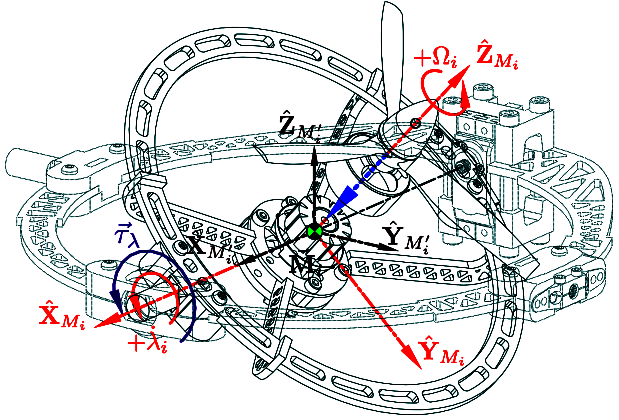
\includegraphics[width=0.65\textwidth]{figs/response-inner}
\caption{Exploded inner ring inertial bodies for $\vec{\tau}_\lambda$}
\label{fig:response-inner}
\vspace{-12pt}
\end{figure}
\par
Deriving dynamic responses for changes in the $\lambda_i$ servo acting on the inner ring frame $\mathcal{F}^{M_i}$ relative to the middle ring frame $\mathcal{F}^{M_i'}$ requires a relative path co-ordinate to be defined. Seeing that the only path variable between the two frames is that servo's rotational position $\lambda_i$ about the $\hat{X}_{M_i}$ axis; the path co-ordinates $\vec{\mathbf{u}}(t)=\begin{bmatrix}\lambda_i&0&0\end{bmatrix}^T$ are used to form the Lagrangian for the inner ring's motion relative the middle ring frame, $\mathcal{L}_{M_i'}\in\mathcal{F}^{M_i'}$.
\par
The inner ring assembly consists of two separate bodies (exploded in Fig:\ref{fig:response-inner}) with relative rotational motion and independent kinetic energies; the rotor assembly with an inertia $J_{r}$ (defined earlier in Eq:\ref{eq:prop-inertia}) and the inner ring (\emph{sans} rotor assembly) which has an inertia $J_{ir}$:
\begin{equation}
J_{ir}=J_{n}-J_{r}=J_{M_i}-J_{r}~~~~\in\mathcal{F}^{M_i}
\end{equation} 
Where $J_n$ or $J_{M_i}$ is the net inertia for the inner ring assembly from Eq:\ref{eq:inertia.inner}. The rotor assembly has an angular velocity $\vec{\omega}_{r/M_i'}$ relative to the middle ring frame $\mathcal{F}^{M_i'}$ from the BLDC motor's rotation $\Omega_i$ and the servo's rate $\dot{\lambda}_i$:
\begin{subequations}\label{eq:angular-rot}
\begin{equation}
\vec{\omega}_{r/M_i'}=R_x(\lambda)\vec{\Omega}_i+\frac{d\lambda}{dt}(\vec{\lambda}_i)~~~~\in\mathcal{F}^{M_i'}
\end{equation}
\vspace{-6pt}
\begin{equation}
=R_x(\lambda)\vec{\Omega}_i+\dot{\vec{\lambda}}_i
\end{equation}
\end{subequations}
With the propeller's angular velocity vector; $\vec{\Omega}_i=\begin{bmatrix}0 & 0 & \Omega_i\end{bmatrix}^T$ in $[\text{rad.s}^{-1}]$, \underline{not in revolutions per second}, and the servo position; $\vec{\lambda}_i=\begin{bmatrix}\lambda_i & 0 & 0\end{bmatrix}^T$ in $[\text{rad}]$. Similarly the inner ring's angular velocity $\vec{\omega}_{M_i/M_i'}$ relative to $\mathcal{F}^{M_i'}$ is only as a result of $\dot{\lambda}_i$:
\begin{equation}\label{eq:angular-inner}
\vec{\omega}_{M_i/M_i'}=\frac{d\lambda}{dt}(\vec{\lambda}_i)=\dot{\vec{\lambda}}_i~~~~\in\mathcal{F}^{M_i'}
\end{equation}
The Lagrangian for the inner ring's energy $\mathcal{L}_{M_i'}$, relative to the middle ring frame $\mathcal{F}^{M_i'}$, consists purely of rotational kinetic energy from angular velocities in Eq:\ref{eq:angular-rot} and Eq:\ref{eq:angular-inner}. The relative potential energy as a result of the rotated center of motion for the inner ring is neglected here as it is already included in Eq:\ref{eq:grav-torque} and shown to simplify out later when considering the entire body system.
\par
Both inertias for the rotor and inner ring bodies, $J_r$ and $J_{ir}$ respectively, are transformed to align with the middle ring frame $\mathcal{F}^{M_i'}$ from an $R_x(\lambda)$ rotation:
\begin{subequations}\label{eq:lagrange-inner}
\begin{equation}\label{eq:lagrange-inner.a}
\mathcal{L}_{M_i'}=\frac{1}{2}\vec{\omega}_{r/M_i'}\text{}^T\big(J_{r}'\big)\vec{\omega}_{r/M_i'}+\frac{1}{2}\vec{\omega}_{M_i/M_i'}\text{}^T\big(J_{ir}'\big)\vec{\omega}_{M_i/M_i'}
\end{equation}
With rotor and inner ring transformed inertias respectively aligned with $\mathcal{F}^{M_i'}$:
\begin{equation}
J_r'= R_x(\lambda)\big(J_r\big)R_x^{-1}(\lambda)~~\text{and}~~J_{ir}'= R_x(\lambda)\big(J_{ir}\big)R_x^{-1}(\lambda)
\end{equation}
Then expanding the Lagrangian $\mathcal{L}_{M_i'}$ in Eq:\ref{eq:lagrange-inner.a}:
\begin{multline}\label{eq:lagrange-inner.b}
\rightarrow\mathcal{L}_{M_i'}=\frac{1}{2}\Big(R_x(\lambda)\vec{\Omega}_i+\dot{\vec{\lambda}}_i\Big)^T\big(R_x(\lambda)\big(J_{r}\big)R_x^{-1}(\lambda)\big)\Big(R_x(\lambda)\vec{\Omega}_i+\dot{\vec{\lambda}}_i\Big)\\+\frac{1}{2}\dot{\vec{\lambda}}_i^{\hspace{2pt}T}\big(R_x(\lambda)\big(J_{ir}\big)R_x^{-1}(\lambda)\big)\dot{\vec{\lambda}}_i
\end{multline}
\end{subequations}
Noting that the inner ring's inertia $J_{ir}$ is now an independent body from the rotor assembly $J_{r}$. Recalling the Euler-Lagrange formulation from Eq:\ref{eq:euler-lagrange} with path co-ordinates $\vec{\mathbf{u}}(t)$ for the inner ring frame, $\mathcal{F}^{M_i}$, relative to  the middle ring frame, $\mathcal{F}^{M_i'}$:
\begin{equation}\label{eq:euler-lagrange-inner}
\frac{d}{dt}\bigg(\frac{\partial \mathcal{L}_{M_i'}}{\partial \dot{\vec{\mathbf{u}}}}\bigg)-\frac{\partial \mathcal{L}_{M_i'}}{\partial \vec{\mathbf{u}}} = \vec{\mathbf{U}} = \vec{\tau}_{\lambda}~~~~\in\mathcal{F}^{M_i'}
\end{equation}
From \cite{rotationlinearize} the partial derivative of a rotation matrix $R_x(\lambda)$ (and by extension the \emph{transformation matrix} $R_x(-\lambda)$) is linearized using a Taylor series expansion. It follows that for some small perturbation $\partial\theta$ away from the nominal $\bar{\theta}$, a generalized rotation matrix about an axis $\hat{u}$ by that angle $\theta$ becomes a first order approximation:
\begin{equation}\label{eq:rotation-linear}
R_u(\bar{\theta}+\partial\theta)\approx\underbrace{\big(1-[\Phi_u(\bar{\theta})\partial\theta]_\times\big)}_{\text{infinitesimal rot}}R_u(\bar{\theta})
\end{equation}
Where $\Phi_u(\theta)$ is a generalized Euler matrix derivative analogous to Eq:\ref{eq:angular-rates.f}. The consequence of Eq:\ref{eq:rotation-linear} is that, for the transformed rotational inertias in Eq:\ref{eq:lagrange-inner}, both $R_x(\lambda)\big(J_r\big)R_x^{-1}(\lambda)$ and $R_x(\lambda)\big(J_{ir}\big)R_x^{-1}(\lambda)$ can be approximated using their instantaneous transformation with no partial derivatives.
\begin{subequations}\label{eq:rot-linearization}
\begin{equation}
R_x(\lambda)\big(J_r\big)R_x^{-1}(\lambda)=J_r'\rightarrow \frac{\partial}{\partial\vec{\mathbf{u}}} J_r' = \frac{\partial}{\partial\vec{\lambda}_i}J_r'\approx 0
\end{equation}
Similarly for the inner ring without the rotor body's contribution:
\begin{equation}
R_x(\lambda)\big(J_{ir}\big)R_x^{-1}(\lambda)=J_{ir}'\rightarrow \frac{\partial}{\partial\vec{\mathbf{u}}} J_{ir}' = \frac{\partial}{\partial\vec{\lambda}_i}J_{ir}'\approx 0
\end{equation}
\end{subequations}
Simplifications in Eq:\ref{eq:rot-linearization} are expanded and shown to be reasonable assumptions next in Sec:\ref{subsec:dynamics.nonlinearities.torque-tests}. It follows that partial derivatives of the Lagrangian Eq:\ref{eq:lagrange-inner} with respect to $\vec{\mathbf{u}}$ are negligible; $\partial\mathcal{L}_{M_i'}/\partial\vec{\mathbf{u}}=0$. Only the partial derivative with respect to the path rate $\dot{\vec{\mathbf{u}}}$ remain. That partial derivative is then:
\begin{equation}\label{eq:3.42b}
\therefore\frac{\partial \mathcal{L}_{M_i'}}{\partial \dot{\vec{\mathbf{u}}}}=\big(J_{r}'\big)\Big(R_x(\lambda)\vec{\Omega}_i+\dot{\vec{\lambda}}_i\Big)+\big(J_{ir}'\big)\dot{\vec{\lambda}}_i
\end{equation}
Transformed inertial derivatives $\dot{J}_r'$ and $\dot{J}_{ir}'$ must first be defined before applying the Euler-Lagrange formulation Eq:\ref{eq:euler-lagrange-inner} to the simplified Lagrangian in Eq:\ref{eq:3.42b}. Those inertial derivatives cannot be separated by time scale from the remainder of Eq:\ref{eq:3.42b} given that $\dot{\lambda}_i$ determines both inertial rates $\dot{J}_r'$ and $\dot{J}_{ir}'$ but is also a component of the kinetic energy in Eq:\ref{eq:lagrange-inner.b}.
\par
Starting with the general case; for some transformed inertia $J$ to be aligned relative to a frame $\mathcal{F}^b$ where the inertia is originally defined with respect to a frame $\mathcal{F}^a$. If the two frames differ by some rotation angle $\theta$ about an Euler axis $\hat{u}$, the generalized rotation matrix from frame $\mathcal{F}^a$ to $\mathcal{F}^b$ is given by $R_{\hat{u}}(\theta)$ calculated from Eq:\ref{eq:rotationoperator}. The transformed inertia is then calculated as:
\begin{subequations}
\begin{equation}
J'=R_{\hat{u}}(\theta)\big(J\big)R_{\hat{u}}^{-1}(\theta)
\end{equation}
Which, from the product rule and the rotation matrix time derivative definition in Eq:\ref{eq:rotation-matrix-derivative}, that transformed inertia has its own derivative:
\begin{equation}
\dot{J}'=\frac{d}{dt}\Big(R_{\hat{u}}(\theta)\big(J\big)R_{\hat{u}}^{-1}(\theta)\Big)=\frac{d}{dt}\Big(R_{\hat{u}}(\theta)\Big)\big(J\big)R_{\hat{u}}^{-1}(\theta)+R_{\hat{u}}(\theta)\big(J\big)\frac{d}{dt}\Big(R_{\hat{u}}^{-1}(\theta)\Big)
\end{equation}
\vspace{-10pt}
\begin{equation}
=[\dot{\vec{\theta}}\hspace{2pt}]_\times R_{\hat{u}}(\theta)\big(J\big)R_{\hat{u}}^{-1}(\theta)-R_{\hat{u}}(\theta)\big(J)[\dot{\vec{\theta}}\hspace{2pt}]_\times R_{\hat{u}}^{-1}(\theta)
\end{equation}
\end{subequations}
Where $\dot{\vec{\theta}}=\dot{\theta}\cdot\hat{u}$ is the angular velocity vector between the two frames. Then both the rotor assembly and inner ring transformed inertias have the derivatives:
\begin{subequations}\label{eq:rotor-deriv}
\begin{equation}
\rightarrow\dot{J}_r'=\frac{d}{dt}\Big(R_x(\lambda)\big(J_r\big)R_x^{-1}(\lambda)\Big)
\end{equation}
\vspace{-10pt}
\begin{equation}
=[\dot{\vec{\lambda}}_i]_\times R_x(\lambda)\big(J_r\big)R_x^{-1}(\lambda)-R_x(\lambda)\big(J_r\big)[\dot{\vec{\lambda}}_i]_\times R_x^{-1}(\lambda)
\end{equation}
\end{subequations}
Similarly for the inner ring's transformed inertial rate $\dot{J}_{ir}'$, without the rotor's contribution, is:
\begin{subequations}\label{eq:inner-deriv}
\begin{equation}
\rightarrow\dot{J}_{ir}'=\frac{d}{dt}\Big(R_x(\lambda)\big(J_{ir}\big)R_x^{-1}(\lambda)\Big)
\end{equation}
\vspace{-12pt}
\begin{equation}
=[\dot{\vec{\lambda}}_i]_\times R_x(\lambda)\big(J_{ir}\big)R_x^{-1}(\lambda)-R_x(\lambda)\big(J_{ir}\big)[\dot{\vec{\lambda}}_i]_\times R_x^{-1}(\lambda)
\end{equation}
\end{subequations}
Inserting those transformed inertial derivatives into Eq:\ref{eq:3.42b} and using Reynolds transportation theorem, Eq:\ref{eq:reynolds} for a vector's derivative in a rotating reference frame. The product rule then yields:
\begin{multline}
\rightarrow \frac{d}{dt} \bigg(\frac{\partial \mathcal{L}_{M_i'}}{\partial \dot{\vec{\mathbf{u}}}}\bigg)=\Big[\big(\dot{J}_r'\big)\big(R_x(\lambda)\vec{\Omega}_i + \dot{\vec{\lambda}}_i\big)+\big(J_{r}'\big)R_x(\lambda)\dot{\vec{\Omega}}_i+\vec{\omega}_{M_i/M_i'}\times \big(J_{r}'\big)R_x(\lambda)\vec{\Omega}_i+\big(J_{r}'\big)\ddot{\vec{\lambda}}_i\\+\vec{\omega}_{M_i/M_i'}\times \big(J_{r}'\big)\dot{\vec{\lambda}}_i\Big]+\Big[\big(\dot{J}_{ir}'\big)\dot{\vec{\lambda}}_i+\big(J_{ir}'\big)\ddot{\vec{\lambda}}_i+\vec{\omega}_{M_i/M_i'}\times \big(J_{ir}'\big)\dot{\vec{\lambda}}_i\Big]=\vec{\mathbf{U}}
\end{multline}
Recombining inertial contributions with the same angular velocity ($J_{r}'+J_{ir}'=J_{n}'$) and recognizing that, from Eq:\ref{eq:angular-inner}, $\vec{\omega}_{M_i/M_i'}=\dot{\vec{\lambda}}$; the generalized net torque encountered by a rotation of $\lambda$ is:
\begin{subequations}
\begin{equation}
\vec{\mathbf{U}}=\big(\dot{J}_r'\big)\vec{\Omega}_i'+\big(J_{r}'\big)\dot{\vec{\Omega}}_i\text{}\hspace{-2pt}'+\dot{\vec{\lambda}}_i\times \big(J_{r}'\big)\vec{\Omega}_i\text{}\hspace{-2pt}'+\big(\dot{J}_{n}'\big)\dot{\vec{\lambda}}_i+\big(J_{n}'\big)\ddot{\vec{\lambda}}_i+\dot{\vec{\lambda}}_i\times \big(J_{n}'\big)\dot{\vec{\lambda}}_i=\vec{\tau}_\lambda~~~~\in\mathcal{F}^{M_i'}
\end{equation}
Where $\vec{\Omega}_i\text{}\hspace{-2pt}'$ and $\dot{\vec{\Omega}}_i\text{}\hspace{-2pt}'$ are the respective transformed angular velocity and acceleration of the propeller in the middle ring frame:
\begin{equation}
\vec{\Omega}_i\text{}\hspace{-2pt}'=R_x(\lambda)\vec{\Omega}_i~~~~\in\mathcal{F}^{M_i'}
\end{equation}
\vspace{-10pt}
\begin{equation}
\dot{\vec{\Omega}}_i\text{}\hspace{-2pt}'=\frac{d\vec{\Omega}}{dt}\big(R_x(\lambda)\vec{\Omega}_i\big)=R_x(\lambda)\dot{\vec{\Omega}}_i~~~~\in\mathcal{F}^{M_i'}
\end{equation}
\end{subequations}
The net torque response from an $\Delta\lambda_i$ rotation, induced in the middle ring frame $\mathcal{F}^{M_i'}$, can be grouped into \emph{inertial rates}, second order \emph{inertial} and first order \emph{gyroscopic} components;
\begin{equation}\label{eq:torque-induced-inner}
\vec{\tau}_\lambda=\underbrace{\big(\dot{J}_{r}'\big)\vec{\Omega}_i\text{}\hspace{-2pt}'+\big(\dot{J}_{n}'\big)\dot{\vec{\lambda}}_i}_{Inertial~rates}+\underbrace{\big(J_r'\big)\dot{\vec{\Omega}}_i\text{}\hspace{-2pt}'+\big(J_{n}'\big)\ddot{\vec{\lambda}}_i}_{Inertial}+\underbrace{\dot{\vec{\lambda}}_i\times \big(J_r'\big)\vec{\Omega}_i\text{}\hspace{-2pt}'+\dot{\vec{\lambda}}_i\times \big(J_{n}'\big)\dot{\vec{\lambda}}_i}_{Gyroscopic}~~~~\in\mathcal{F}^{M_i'}
\end{equation}
\par
Similarly for the middle ring frame $\mathcal{F}^{M_i'}$ relative to the intermediary frame $\mathcal{F}^{M_i''}$, the only relative path variable is $\vec{\mathbf{v}}(t)=\begin{bmatrix}0 & \alpha_i & 0\end{bmatrix}^T$. The entire motor module structure consists of three separate rotating bodies each with their own relative angular velocities; the \emph{rotor} assembly, \emph{inner} and \emph{middle} ring structures (exploded in Fig:\ref{fig:response-middle}).
\begin{figure}[htbp]
\centering
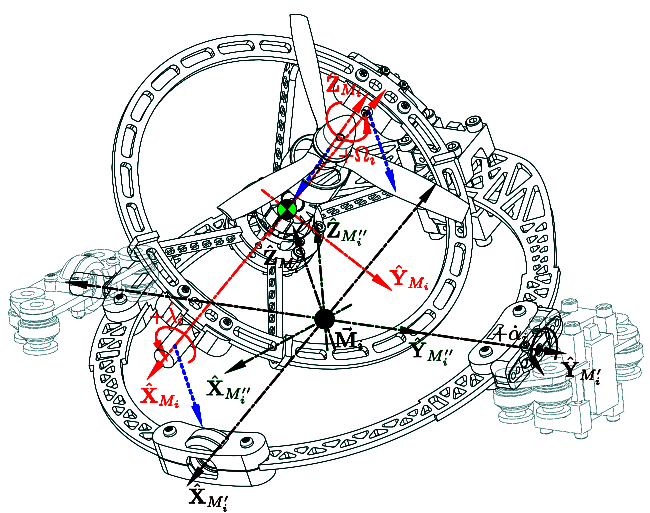
\includegraphics[width=0.75\textwidth]{figs/response-middle}
\caption{Exploded middle ring inertial bodies for $\vec{\tau}_{\alpha}$}
\label{fig:response-middle}
\vspace{-16pt}
\end{figure}
\par
Following the same process to evaluate the $ \alpha_i$ servo's response the middle ring assembly Lagrangian $\mathcal{L}_{M_i''}$ is formed, but with respect to the intermediary frame $\mathcal{F}^{M_i''}$. First transforming the inertias; the rotor assembly, further rotated by $\alpha_i$ about its $\hat{Y}_{M_i'}$, has an inertia aligned with axes in $\mathcal{F}^{M_i''}$:
\begin{subequations}
\begin{equation}\label{eq:rotor-inertia-mid}
J_r''=R_y(\alpha)\big(J_r'\big)R_y^{-1}(\alpha)=R_y(\alpha)R_x(\lambda)\big(J_r\big)R_x^{-1}(\lambda)R_y^{-1}(\alpha)~~~~\in\mathcal{F}^{M_i''}
\end{equation}
Which has a derivative $\dot{J}_r''$:
\begin{equation}\label{eq:rotor-inertia-rate}
\dot{J}_r''=R_y(\alpha)\big(\dot{J}_r'\big)R_y^{-1}(\alpha)+[\dot{\vec{\alpha}}_i]_\times R_y(\alpha)\big(J_r'\big)R_y^{-1}(\alpha)-R_y(\alpha)\big(J_r'\big)[\dot{\vec{\alpha}}_i]_\times R_y^{-1}(\alpha)
\end{equation}
\end{subequations}
The inner ring structure has an inertia, still \emph{without} including the rotor assembly:
\begin{subequations}
\begin{equation}\label{eq:inner-inertia-mid}
J_{ir}''=R_y(\alpha)\big(J_{ir}'\big)R_y^{-1}(\alpha)=R_y(\alpha)R_x(\lambda)\big(J_{ir}\big)R_x^{-1}(\lambda)R_y^{-1}(\alpha)~~~~\in\mathcal{F}^{M_i''}
\end{equation} 
Similarly with a derivative $\dot{J}_{ir}''$:
\begin{equation}\label{eq:inner-inertia-rate}
\dot{J}_{ir}''=R_y(\alpha)\big(\dot{J}_{ir}'\big)R_y^{-1}(\alpha)+[\dot{\vec{\alpha}}\hspace{2pt}]_\times R_y(\alpha)\big(J_{ir}'\big)R_y^{-1}(\alpha)-R_y(\alpha)\big(J_{ir}'\big)[\dot{\vec{\alpha}}\hspace{2pt}]_\times R_y^{-1}(\alpha)
\end{equation}
\end{subequations}
Finally the middle ring structure's inertia from Eq:\ref{eq:inertia.middle.a}, with neither the rotor's nor the inner ring's contributions:
\begin{subequations}
\begin{equation}\label{eq:middle-inertia-mid}
J_m'=R_y(\alpha)\big(J_\text{m}\big)R_y^{-1}(\alpha)
\end{equation}
Which, when using the collective motor module inertia $J_p$ from Eq:\ref{eq:inertia.middle.b}, expands to:
\begin{equation}
=R_y(\alpha)\big(J_\text{p}\big)R_y^{-1}(\alpha)-R_y(\alpha)R_x(\lambda)\big(J_\text{n}\big)R_x^{-1}(\lambda)R_y^{-1}(\alpha)
\end{equation}
\vspace{-12pt}
\begin{equation}\label{eq:middle-inertia-relation}
=J_\text{p}'-J_{n}''=J_\text{p}'-\big(J_{ir}''+J_{r}''\big)~~~~\in\mathcal{F}^{M_i''}
\end{equation}
Which has a derivative purely as a result of $\dot{\alpha}$:
\begin{equation}
\dot{J}_m'=[\dot{\vec{\alpha}}_i]_\times R_y(\alpha)\big(J_m\big)R_y^{-1}(\alpha)-R_y(\alpha)\big(J_m\big)[\dot{\vec{\alpha}}_i]_\times R_y^{-1}(\alpha)
\end{equation}
However; that derivative $\dot{J}_m'$, using $\dot{J}_{r}''$ and $\dot{J}_{ir}''$ from Eq:\ref{eq:rotor-inertia-rate} and Eq:\ref{eq:inner-inertia-rate} respectively, expands to:
\begin{equation}\label{eq:middle-inertia-rate}
\dot{J}_m'=[\dot{\vec{\alpha}}_i]_\times R_y(\alpha)\big(J_p\big)R_y^{-1}(\alpha)-R_y(\alpha)\big(J_p\big)[\dot{\vec{\alpha}}_i]_\times R_y^{-1}(\alpha)-(\dot{J}_{ir}''+\dot{J}_{r}'')
\end{equation}
\end{subequations}
Note that introducing the relations of Eq:\ref{eq:middle-inertia-relation} and Eq:\ref{eq:middle-inertia-rate} to the collective body inertia $J_p$ is to simplify the subsequent equations. Each body then has its own relative angular velocity with respect to the intermediate frame $\mathcal{F}^{M_i''}$. For the rotor; $\vec{\omega}_{r/M_i''}$ is the relative angular velocity of that assembly from the motor $\Omega_i$ and servo rates $\dot{\lambda}_i$ and $\dot{\alpha}_i$:
\begin{subequations}\label{eq:rotor-relative}
\begin{equation}
\vec{\omega}_{r/M_i''}=R_y(\alpha)R_x(\lambda)\vec{\Omega}_i+\frac{d\lambda}{dt}\Big(R_y(\alpha)\vec{\lambda}_i\Big)+\frac{d\alpha}{dt}\big(\vec{\alpha}_i\big)~~~~\in\mathcal{F}^{M_i''}
\end{equation}
\vspace{-12pt}
\begin{equation}
=R_y(\alpha)R_x(\lambda)\vec{\Omega}_i+R_y(\alpha)\dot{\vec{\lambda}}_i+\dot{\vec{\alpha}}_i
\end{equation}
\vspace{-12pt}
\begin{equation}
\rightarrow \vec{\omega}_{r/M_i''}=\vec{\Omega}_i\text{}\hspace{-2pt}''+\dot{\vec{\lambda}}_i\text{}\hspace{-2pt}'+\dot{\vec{\alpha}}_i
\end{equation}
\end{subequations}
Where $\vec{\Omega}_i''$ and $\dot{\vec{\lambda}}_i'$ are respectively propeller and servo velocities transformed to the frame $\mathcal{F}^{M_i''}$. Next, the inner ring has an angular velocity $\vec{\omega}_{M_i/M_i''}$ relative to the intermediate frame $\mathcal{F}^{M_i''}$ from servo rates $\dot{\lambda}_i$ and $\dot{\alpha}_i$:
\begin{subequations}\label{eq:inner-relative}
\begin{equation}
\vec{\omega}_{M_i/M_i''}=\frac{d\lambda}{dt}\big(R_y(\alpha)\vec{\lambda}_i\big)+\frac{d\alpha}{dt}(\vec{\alpha}_i)~~~~\in\mathcal{F}^{M_i''}
\end{equation}
\vspace{-10pt}
\begin{equation}
=R_y(\alpha)\dot{\vec{\lambda}}_i+\dot{\vec{\alpha}}_i=\dot{\vec{\lambda}}_i\text{}\hspace{-2pt}'+\dot{\vec{\alpha}}_i
\end{equation}
\end{subequations}
Finally the middle ring has an angular velocity $\vec{\omega}_{M_i'/M_i''}$ relative to the intermediary frame only as a result of $\dot{\alpha}_i$:
\begin{equation}\label{eq:middle-relative}
\vec{\omega}_{M_i'/M_i''}=\frac{d\alpha}{dt}(\vec{\alpha}_i)=\dot{\vec{\alpha}}_i~~~~\in\mathcal{F}^{M_i''}
\end{equation}
Using the relative path co-ordinate $\vec{\mathbf{v}}(t)$, the Lagrangian $\mathcal{L}_{M_i''}$ can be constructed for the combined motor module relative to the frame $\mathcal{F}^{M_i''}$ with kinetic energies of the rotor assembly, inner and middle ring structures respectively:
\begin{equation}\label{eq:alpha-lagrange}
\mathcal{L}_{M_i''}=\frac{1}{2}\vec{\omega}_{r/M_i''}^{\hspace{2pt}T}\big(J_{r}''\big)\vec{\omega}_{r/M_i''}+\frac{1}{2}\vec{\omega}_{M_i/M_i''}^{\hspace{2pt}T}\big(J_{ir}''\big)\vec{\omega}_{M_i/M_i''}+\frac{1}{2}\vec{\omega}_{M_i'/M_i''}^{\hspace{2pt}T}\big(J_{m}'\big)\vec{\omega}_{M_i'/M_i''}
\end{equation}
Where Eq:\ref{eq:alpha-lagrange} again does not include any potential gravitational energies as such quantities were already accounted for in Eq:\ref{eq:grav-torque}. Therefore the Langragian from Eq:\ref{eq:alpha-lagrange} expands to:
\begin{multline}\label{eq:alpha-lagrange-two}
\therefore\mathcal{L}_{M_i''}=\frac{1}{2}\Big[R_y(\alpha)R_x(\lambda)\vec{\Omega}_i+R_y(\alpha)\dot{\vec{\lambda}}_i+\dot{\vec{\alpha}}\Big]^T\big(J_r''\big)\Big[R_y(\alpha)R_x(\lambda)\vec{\Omega}_i+Ry(\alpha)\dot{\vec{\lambda}}_i+\dot{\vec{\alpha}}_i\Big]\\
+\frac{1}{2}\Big[R_y(\alpha)\dot{\vec{\lambda}}_i+\dot{\vec{\alpha}}_i\Big]^T\big(J_{ir}''\big)\Big[R_y(\alpha)\dot{\vec{\lambda}}_i+\dot{\vec{\alpha}}_i\Big]
+\frac{1}{2}\dot{\vec{\alpha}}_i^{\hspace{2pt}T}\big(J_m'\big)\dot{\vec{\alpha}}_i
\end{multline}
Again, justifying the rotation matrix linearization using Eq:\ref{eq:rotation-linear}, matrices $J_r''$, $J_{ir}''$ and $J_m'$ are all instantaneous transformed inertias. The Euler-Lagrange formulation then simplifies, with the partial derivative $\partial\mathcal{L}_{M_i''}/\partial\vec{\mathbf{v}}=0$, to:
\begin{equation}
\frac{d}{dt}\Bigg(\frac{\partial\mathcal{L}_{M_i''}}{\partial\dot{\vec{\mathbf{v}}}}\Bigg)-\frac{\partial\mathcal{L}_{M_i''}}{\partial\vec{\mathbf{v}}}=\frac{d}{dt}\Bigg(\frac{\partial\mathcal{L}_{M_i''}}{\partial\dot{\vec{\mathbf{v}}}}\Bigg)=\vec{\mathbf{V}}=\vec{\tau}_\alpha
\end{equation}
Finding the partial derivative of the Lagrangian $\mathcal{L}_{M_i''}$ with respect to $\dot{\vec{\mathbf{v}}}$ yields:
\begin{subequations}
\begin{equation}
\frac{\partial\mathcal{L}_{M_i''}}{\partial\dot{\vec{\mathbf{v}}}}=\big(J_r''\big)\Big[\vec{\Omega}_i\hspace{-2pt}''+\dot{\vec{\lambda}}_i\hspace{-2pt}'+\dot{\vec{\alpha}}_i\Big]+\big(J_{ir}''\big)\Big[\dot{\vec{\lambda}}_i\hspace{-2pt}'+\dot{\vec{\alpha}}_i\Big]+\big(J_m'\big)\dot{\vec{\alpha}}_i
\end{equation}
Which, with relative angular velocity definitions from Eq:\ref{eq:rotor-relative},\ref{eq:inner-relative} and \ref{eq:middle-relative}, expands to:
\begin{equation}
=\big(J_r''\big)\Big[R_y(\alpha)R_x(\lambda)\vec{\Omega}_i+R_y(\alpha)\dot{\vec{\lambda}}_i+\dot{\vec{\alpha}}_i\Big]+\big(J_{ir}''\big)\Big[R_y(\alpha)\dot{\vec{\lambda}}_i+\dot{\vec{\alpha}}_i\Big]+\big(J_m'\big)\dot{\vec{\alpha}}_i
\end{equation}
Then taking the Lagrangian's time derivative and using inertial rates Eq:\ref{eq:rotor-inertia-rate},\ref{eq:inner-inertia-rate} and \ref{eq:middle-inertia-rate}; split into product ruled derivative components:
\begin{multline}\label{eq:alpha-lagrange-deriv}
\rightarrow \frac{d}{dt}\Bigg(\frac{\partial \mathcal{L}_{M_i''}}{\partial\dot{\vec{\mathbf{v}}}}\Bigg)=\Big[\big(\dot{J}_r''\big)(\vec{\Omega}_i\hspace{-2pt}''+\dot{\vec{\lambda}}_i\hspace{-2pt}'+\dot{\vec{\alpha}}_i)\Big]
\\
+\Big[\big(J_r''\big)\dot{\vec{\Omega}}_i\hspace{-2pt}''+\vec{\omega}_{M_i/M_i''}\times\big(J_r''\big)\vec{\Omega}_i\hspace{-2pt}''+\big(J_r''\big)\ddot{\vec{\lambda}}_i\hspace{-2pt}'+\vec{\omega}_{M_i/M_i''}\times \big(J_r''\big)\dot{\vec{\lambda}}_i\hspace{-2pt}'+\big(J_r''\big)\ddot{\vec{\alpha}}_i+\vec{\omega}_{M_i'/M_i''}\times \big(J_r''\big)\dot{\vec{\alpha}}_i\Big]
\\
+\Big[\big(\dot{J}_{ir}''\big)(\dot{\vec{\lambda}}_i\hspace{-2pt}'+\dot{\vec{\alpha}}_i)\Big]
+\Big[\big(J_{ir}''\big)\ddot{\vec{\lambda}}_i\hspace{-2pt}'+\vec{\omega}_{M_i/M_i''}\times\big(J_{ir}''\big)\dot{\vec{\lambda}}_i\hspace{-2pt}'+\big(J_{ir}''\big)\ddot{\vec{\alpha}}_i+\vec{\omega}_{M_i'/M_i''}\times\big(J_{ir}''\big)\dot{\vec{\alpha}}_i\Big]
\\
+\Big[\big(\dot{J}_m'\big)\dot{\vec{\alpha}}_i\Big] +\Big[\big(J_m'\big)\ddot{\vec{\alpha}}_i+\vec{\omega}_{M_i'/M_i''}\times\big(J_m'\big)\dot{\vec{\alpha}}_i\Big]
\end{multline}
With relative frame angular velocities; $\vec{\omega}_{M_i/M_i''}$ of the inner ring relative to the intermediate frame, and $\vec{\omega}_{M_i'/M_i''}$ of the middle ring relative to the intermediate frame. Both are defined respectively as:
\begin{equation}
\vec{\omega}_{M_i/M_i''}=R_y(\alpha)\dot{\vec{\lambda}}_i+\dot{\vec{\alpha}}_i=\dot{\vec{\lambda}}_i\hspace{-2pt}'+\dot{\vec{\alpha}}_i~~~~\in\mathcal{F}^{M_i''}
\end{equation}
\vspace{-16pt}
\begin{equation}
\vec{\omega}_{M_i'/M_i''}=\dot{\vec{\alpha}}_i~~~~\in\mathcal{F}^{M_i''}
\end{equation}
\par
Eq:\ref{eq:alpha-lagrange-deriv} is an ominous and incredibly complex result to try expand and make sense of. However it can be simplified; recognizing that Eq:\ref{eq:alpha-lagrange-deriv} contains kinetic energies already introduced in Eq:\ref{eq:torque-induced-inner}, but transformed to the frame $\mathcal{F}^{M_i''}$. After some mathematics, Eq:\ref{eq:alpha-lagrange-deriv} can be simplified with responses pertinent to $\Delta\alpha_i$ and then the transformed generalized force response $R_y(\alpha)\vec{\tau}_\lambda$:
\begin{multline}\label{eq:3.63f}
\vec{\mathbf{V}}=R_y(\alpha)\frac{d}{dt}\Big(\frac{\partial\mathcal{L}_{M_i'}}{\partial\dot{\vec{\mathbf{u}}}}\Big)+\Big(R_y(\alpha)\big(\dot{J}_r'\big)R_y^{-1}(\alpha)\Big)\dot{\vec{\alpha}}+\Big(\dot{J}_r''-R_y(\alpha)\big(\dot{J}_r'\big)R_y^{-1}(\alpha)\Big)\big(\vec{\Omega}_i''+\dot{\vec{\lambda}}_i'+\dot{\vec{\alpha}}_i\big)+\big(J_r''\big)\ddot{\vec{\alpha}}_i
\\
+\dot{\vec{\alpha}}_i\times\big(J_r''\big)\Big(\vec{\Omega}_i''+\dot{\vec{\lambda}}_i'+\dot{\vec{\alpha}}_i\Big)+\Big(R_y(\alpha)\big(\dot{J}_{ir}'\big)R_y^{-1}(\alpha)\Big)\dot{\vec{\alpha}}+\Big(\dot{J}_{ir}''-R_y(\alpha)\big(\dot{J}_{ir}'\big)R_y^{-1}(\alpha)\Big)\big(\dot{\vec{\lambda}}_i'+\dot{\vec{\alpha}}_i\big)
\\
+\big(J_{ir}''\big)\ddot{\vec{\alpha}}_i+\dot{\vec{\alpha}}_i\times \big(J_{ir}''\big)\Big(\dot{\vec{\lambda}}_i\hspace{-2pt}'+\dot{\vec{\alpha}}_i\Big)+\big(\dot{J}_m'\big)\dot{\vec{\alpha}}_i+\big(J_m'\big)\ddot{\vec{\alpha}}_i+\dot{\vec{\alpha}}_i\times \big(J_m'\big)\dot{\vec{\alpha}}_i
\end{multline}
Paying special attention to differentiate $\dot{J}_{r}''$ and $\dot{J}_{ir}''$ from Eq:\ref{eq:rotor-inertia-rate} and Eq:\ref{eq:inner-inertia-rate} respectively with $R_y(\alpha)\big(\dot{J}_r'\big)R_y^{-1}(\alpha)$ and $R_y(\alpha)\big(\dot{J}_{ir}'\big)R_y^{-1}(\alpha)$. Where the latter two are inertia rates from Eq:\ref{eq:rotor-deriv} and Eq:\ref{eq:inner-deriv} both transformed to the frame $\mathcal{F}^{M_i''}$. 
\par
The complex result in Eq:\ref{eq:3.63f} can be further simplified by introducing combined inertial bodies $J_n=J_r+J_{ir}$ for the \emph{entire} inner ring, Eq:\ref{eq:inertia.inner}, and $J_p=J_m+R_x(\lambda)\big(J_n\big)R_x^{-1}(\lambda)$ for the \emph{entire} motor module's inertia, Eq:\ref{eq:inertia.middle.b}. Using $J_p'=R_y(\alpha)\big(J_p\big)R_y^{-1}(\alpha)$ and $J_n'=R_y(\alpha)\big(J_n\big)R_y^{-1}(\alpha)$ for the net modules inertia and the entire inner ring inertia both respectively aligned with the frame $\mathcal{F}^{M_i''}$:
\begin{multline}
\rightarrow\vec{\mathbf{V}}=R_y(\alpha)\frac{d}{dt}\bigg(\frac{\partial\mathcal{L}_{M_i'}}{\partial\dot{\vec{\mathbf{u}}}}\bigg)+\Big(R_y(\alpha)\big(\dot{J}_n'\big)R_y(\alpha)\Big)\dot{\vec{\alpha}}_i+ \Big(\dot{J}_p'-R_y(\alpha)\big(\dot{J}_p\big)R_y^{-1}(\alpha)\Big)\dot{\vec{\alpha}}_i
\\
+\Big(\dot{J}_n''-R_y(\alpha)\big(\dot{J}_n'\big)R_y^{-1}(\alpha)\Big)\dot{\vec{\lambda}}'+\Big(\dot{J}_r''-R_y(\alpha)\big(\dot{J}_r'\big)R_y^{-1}(\alpha)\Big)\vec{\Omega}_i''
\\
+J_p'\ddot{\vec{\alpha}}_i+\dot{\vec{\alpha}}_i\times\Big(\big(J_p'\big)\dot{\vec{\alpha}}+\big(J_n''\big)\dot{\vec{\lambda}}_i'+\big(J_r''\big)\vec{\Omega}_i''\Big)
\end{multline}
\end{subequations}
Noting that $\dot{J}_p = \dot{J}_r'+\dot{J}_{ir}'+\dot{J}_m$ and that $\dot{J}_m=0$, it follows that $\dot{J}_p =\dot{J}_n'$. Then isolating the torque response from $\Delta\alpha$, and again grouping inertial bodies with shared angular velocities together. The \emph{inertial rates}, second order \emph{inertial} and first order \emph{gyroscopic} responses are then:
\begin{multline} \label{eq:torque-induced-middle}
\vec{\tau}_\alpha(\lambda_i)=\underbrace{\big(\dot{J}_p'\big)\dot{\vec{\alpha}}_i+\Big(\dot{J}_n''-R_y(\alpha)\big(\dot{J}_n'\big)R_y^{-1}(\alpha)\Big)\dot{\vec{\lambda}}_i'+\Big(\dot{J}_r''-R_y(\alpha)\big(\dot{J}_r'\big)R_y^{-1}(\alpha)\Big)\vec{\Omega}_i''}_{Inertial~rates}
\\
+\underbrace{\big(J_\text{p}'\big)\ddot{\vec{\alpha}}_i}_{Inertial}+\underbrace{\dot{\vec{\alpha}}_i\times \Big(\big(J_p'\big)\dot{\vec{\alpha}}_i+\big(J_n''\big)\dot{\vec{\lambda}}_i\hspace{-2pt}'+\big(J_r''\big)\vec{\Omega}_i\hspace{-2pt}''\Big)}_{Gyroscopic}~~~~\in\mathcal{F}^{M_i''}
\end{multline}
Careful inspection could have yielded the inertial and gyroscopic components of both Eq:\ref{eq:torque-induced-inner} and Eq:\ref{eq:torque-induced-middle}, however the effect of inertial rates on the torque system is a far less obvious result. The assumption in Eq:\ref{eq:rotation-linear} that rotated inertias can be linearized is shown to hold true next in Sec:\ref{subsec:dynamics.nonlinearities.torque-tests} where simulations and physical tests corroborate the above models.
\par
Both servo's respective induced torques, $\vec{\tau}_\lambda$ and $\vec{\tau}_\alpha(\lambda_i)$, occur in sequential gimbal-like frames. The opposing negative responses to induced relative rotations effect the angular state dynamics in Eq:\ref{eq:states.d}, and must be transformed to the common body frame.
\begin{equation}\label{eq:torque-response}
\vec{\tau}_Q(u)=-\sum_{i=1}^4 \Big(R_z(\sigma)R_y(\alpha)\vec{\tau}_{\lambda}(i)+R_z(\sigma)\vec{\tau}_{\alpha}(\lambda_i)\Big)~~~~[\text{N.m}],~\in\mathcal{F}^b
\end{equation}
\par
The final non-trivial torque term to account for is as a result of the response which relative rotations $\lambda_i$ and $\alpha_i$ have to the net angular velocity of the entire multibody system $\vec{\omega}_b$. Such responses are an extension of the fundamental rigid 6-DOF differential equation for angular motion, reiterated from Eq:\ref{eq:angular-multibody}:
\begin{equation}
\dot{\vec{\omega}}_b=\big(J_b^{-1}\big)\Big(-\vec{\omega}_b\times\big(J_b\big)\vec{\omega}_b+\vec{\tau}_{\mu}\Big)~~~~[\text{rad.s}^{\text{-}s}],~\in\mathcal{F}^b
\end{equation}
\par
Before continuing with a Lagrangian formulation applied to the entire multibody system; it is worth first establishing a Lemma to add some clarity to the steps which follow. Consider the hypothetical, non-inertial, 2-D system illustrated in Fig:\ref{fig:lemma-1}. A massless rod of length $r$ connects a rotational body, with a mass $m_b$ at point $\mathbf{B}$, to a center point $\mathbf{O}$. The principle frame $\mathcal{F}^{1}$ has axes $\hat{X}_1$ and $\hat{Y}_1$ as illustrated. The arm has a rotational velocity $\dot{\phi}$ relative to $\mathcal{F}^{1}$, applied by some "motor". Attached to the end of the rod is a secondary frame $\mathcal{F}^2$ with an $\hat{X}_2$ axis co-linear to the rod and a perpendicular $\hat{Y}_2$. The rotational body, centered at $\mathbf{B}$, has a rotational inertia $J_\mathbf{B}$ about the point (or axis) $\mathbf{B}$. That rotating body has a rotational velocity $\dot{\theta}$ from another "motor" relative to $\mathcal{F}^2$; the question is then how to find the net torque acting on the system in terms of angular accelerations $\ddot{\phi}$ and $\ddot{\theta}$?
\begin{figure}[htbp]
\centering
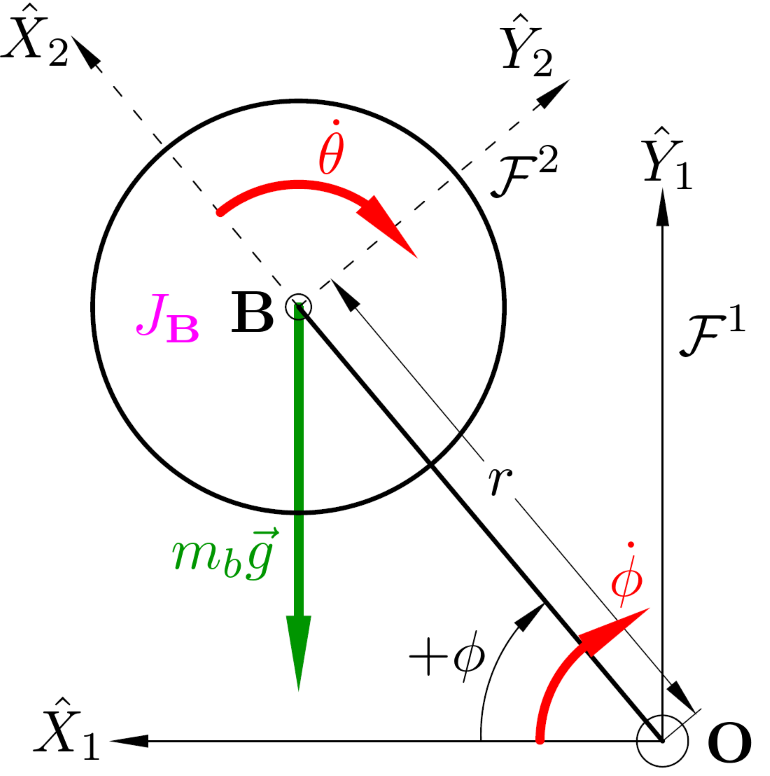
\includegraphics[width=0.4\textwidth]{figs/lemma-1}
\caption{Rotating system}
\label{fig:lemma-1}
\vspace{-18pt}
\end{figure} 
\par
Isolated free body diagrams for each body under consideration are illustrated in Fig:\ref{fig:lemma}. Starting with the rotational body, Fig:\ref{fig:lemma-a}, the torque acting about point $\mathbf{B}$ is simply an inertial response to combined angular accelerations $\ddot{\theta}$ and $\ddot{\alpha}$:
\begin{equation}
\tau_\mathbf{B}=-\tau_\theta=-J_b(\ddot{\theta}+\ddot{\phi})
\end{equation}
The net force is purely the gravitational force acting at point $\mathbf{B}$ as a result of the mass $m_b$:
\begin{equation}
F_\mathbf{B}=-G=-m_b\vec{g}
\end{equation}
That torque and force pair, $F_\mathbf{B}$ and $\tau_\mathbf{B}$, are transferred to the massless rod connecting through point $\mathbf{B}$ to $\mathbf{O}$, Fig:\ref{fig:lemma-b}. The net torque acting around point $\mathbf{O}$ is then comprised of three components; inferred torque from $\tau_\mathbf{B}$, a torque arm from force $F_\mathbf{B}$ and an inertial torque response to the effective "point-mass" at point $\mathbf{B}$ relative to $\mathbf{O}$:
\begin{equation}
\tau_\mathbf{O}=-\tau_\phi=-\tau_\mathbf{B}-F_\mathbf{B}r\cos{\phi}+m_br^2(\ddot{\phi})
\end{equation}
\par
\begin{figure}[htbp]
\centering
\begin{subfigure}{0.49\textwidth}
\centering
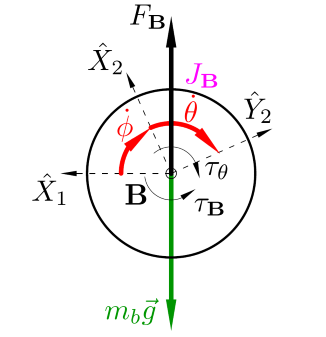
\includegraphics[width=\textwidth]{figs/lemma-a}
\caption{Rotational body}
\label{fig:lemma-a}
\end{subfigure}
\begin{subfigure}{0.49\textwidth}
\centering
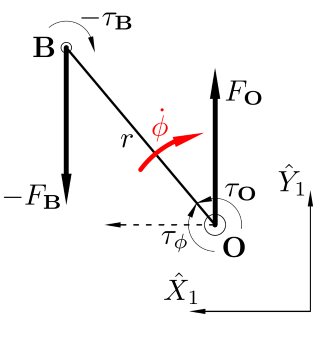
\includegraphics[width=\textwidth]{figs/lemma-b}
\caption{Massless rod}
\label{fig:lemma-b}
\end{subfigure}
\caption{Free-body diagram for rotational system}
\label{fig:lemma}
\vspace{-10pt}
\end{figure}
The net response force acting at point $\mathbf{O}$, $F_\mathbf{O}$, is of no consequence to the calculation of net torques. The "motor" applies a torque $\tau_\phi$ to the rod to induce some angular acceleration $\ddot{\phi}$ on the whole system. Opposed to that angular acceleration is the torque $\tau_\mathbf{O}$ which acts against that "motor". The torque $\tau_\phi$ acting on the system can then be simplified:
\begin{equation}
\tau_\phi=J(\ddot{\theta}+\ddot{\phi})+m_br^2(\ddot{\phi})-m_b\vec{g}r\cos\phi
\end{equation}
That result would not be as obvious when inferred from an energy equation. The equivalent Lagrangian for net kinetic and potential energy of the system, $T$ and $U$ respectively, would be:
\begin{subequations}
\begin{equation}
\mathcal{L}=T(\theta,\phi)-U(\theta,\phi)
\end{equation}
\vspace{-14pt}
\begin{equation}\label{eq:lemma-lagrange}
\mathcal{L}=\frac{1}{2}\vec{\omega}_\mathbf{B}^T\big(J_\mathbf{B}\big)\vec{\omega}_\mathbf{B}+\frac{1}{2}\vec{\omega}_\mathbf{O}^T\big(J_\mathbf{O}\big)\vec{\omega}_\mathbf{O}-m_b\vec{g}r\sin{\phi}
\end{equation}
Where $\vec{\omega}_\mathbf{B}$ and $\vec{\omega}_\mathbf{O}$ are net angular velocities of the rotational body and massless connection rod respectively. The important thing to consider is that $J_\mathbf{O}$, the net rotational inertia about the point $\mathbf{O}$, is simply the point mass inertia $m_br^2$ and \underline{\emph{NOT}} the expected parallel axis theorem $J_\mathbf{O}\not=J_\mathbf{B}'=J_\mathbf{B}+m_br^2$. Expanding Eq:\ref{eq:lemma-lagrange} and applying the Euler-Lagrange formulation yields:
\begin{equation}
\rightarrow\mathcal{L}=\frac{1}{2}\Big(\dot{\theta}+\dot{\phi}\Big)^T\big(J_\mathbf{B}\big)\Big(\dot{\theta}+\dot{\phi}\Big)+\Big(\dot{\phi}\Big)\big(m_br^2\big)\Big(\dot{\phi}\Big)-m_b(-g)r\sin\phi
\end{equation}
\vspace{-10pt}
\begin{equation}
\therefore\text{Genealized forces}=\frac{d}{dt}\Big(\frac{\partial\mathcal{L}}{\partial\dot{\phi}}\Big)-\frac{\partial\mathcal{L}}{\partial\phi}=\vec{\tau}_\phi
\end{equation}
\vspace{-8pt}
\begin{equation}
=\frac{d}{dt}\bigg(\big(J_\mathbf{B}\big)\Big(\dot{\theta}+\dot{\phi}\Big)+\big(m_br^2\big)\Big(\dot{\phi}\Big)\bigg)-m_bgr\cos\phi
\end{equation}
\vspace{-8pt}
\begin{equation}
\therefore\tau_\phi=J_\mathbf{B}(\ddot{\theta}+\ddot{\phi})+m_br^2(\ddot{\phi})-m_bgr\cos\phi
\end{equation}
\vspace{-12pt}
\begin{equation}\label{eq:lemma-torque}
=J_b\ddot{\theta}+J_b'\ddot{\phi}+\tau_g
\end{equation}
\end{subequations}
Where $J_b'$ \underline{is the parallel axis} inertia and $\tau_g$ is the gravitational torque arm contribution. The above then leads to the corollary ascertained from the system in Fig:\ref{fig:lemma-1}:
\begin{lemma}\label{lem:1}
A torque response opposed to angular acceleration of a doubly rotating body can be found as the contribution of the principle rotational inertia about the first axis of rotation with \underline{only} the first rotational acceleration and a parallel axis inertia about the second rotational axis with the second, independent rotational velocity.
\par
Or the same torque can be found as the inertial opposition to net angular acceleration (sum of both rotations) about the first axis and a point mass inertia opposed to the second rotation about its respective axis.
\end{lemma}
\par
Returning then to the net multibody system and separating the motor module from the entire body structure first (exploded bodies for \emph{motor module 1} in Fig:\ref{fig:response-body}). Considering only the additional contribution $\vec{\omega}_b$ has on a singular motor module and later introducing the entire combined system; the Lagrangian derivation for motion relative to the inertial frame then follows\ldots
\begin{figure}[htbp]
\centering
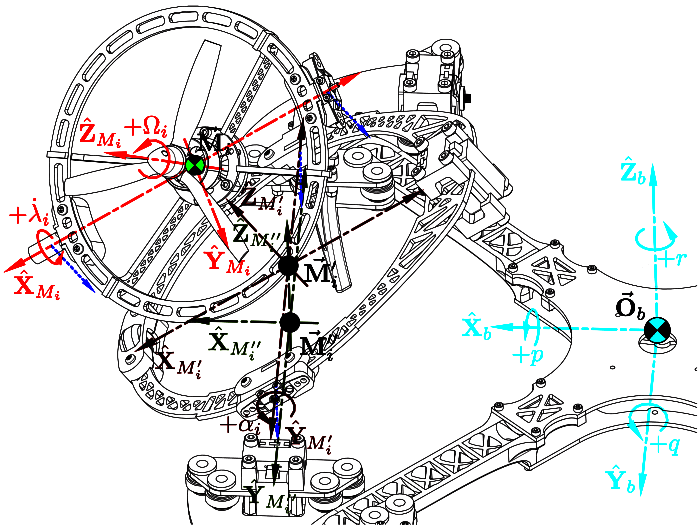
\includegraphics[width=0.9\textwidth]{figs/response-body}
\vspace{-5pt}
\caption{Exploded motor module inertial bodies for $\vec{\omega}_b$ response}
\label{fig:response-body}
\vspace{-18pt}
\end{figure}
\par
The relative $\hat{Z}_{M_i''}$ rotation is what differentiates the intermediate frame $\mathcal{F}^{M_i''}$ (used for calculations pertinent to Fig:\ref{fig:response-middle}) and the body frame $\mathcal{F}^b$. The now familiar rotor assembly, inner and middle ring structure's inertias from Eq:\ref{eq:rotor-inertia-mid},\ref{eq:inner-inertia-mid} and \ref{eq:middle-inertia-mid} have respective counterparts aligned with $\mathcal{F}^b$:
\begin{subequations}\label{eq:module-inertia-body}
\begin{equation}
J_r'''=R_z(\sigma)\big(J_r''\big)R_z^{-1}(\sigma)=R_z(\sigma)R_y(\alpha)R_x(\lambda)\big(J_r\big)R_x^{-1}(\lambda)R_y^{-1}(\alpha)R_z^{-1}(\sigma)
\end{equation}
\vspace{-10pt}
\begin{equation}
J_{ir}'''=R_z(\sigma)\big(J_{ir}''\big)R_z^{-1}(\sigma)=R_z(\sigma)R_y(\alpha)R_x(\lambda)\big(J_{ir}\big)R_x^{-1}(\lambda)R_y^{-1}(\alpha)R_z^{-1}(\sigma)
\end{equation}
\vspace{-10pt}
\begin{equation}
J_m''=R_z(\sigma)\big(J_m'\big)R_z^{-1}(\sigma)=R_z(\sigma)R_y(\alpha)\big(J_m\big)R_y^{-1}(\alpha)R_z^{-1}(\sigma)
\end{equation}
\end{subequations}
Where $\sigma_i$ in Eq:\ref{eq:module-inertia-body} is the relative orthogonal $\hat{Z}_{M_i''}$ difference between frames $\mathcal{F}^{M_i''}$ and $\mathcal{F}^b$ defined before in Eq:\ref{eq:motor-module-rotation} and illustrated previously in Fig:\ref{fig:body-frame}. Because $\sigma_i$ is constant for each $i\in[1:4]$, the inertial rate for each component of the motor module is simply transformations of $\dot{J}_r''$,$\dot{J}_{ir}''$ and $\dot{J}_m'$ previously in Eq:\ref{eq:rotor-inertia-rate},\ref{eq:inner-inertia-rate} and \ref{eq:middle-inertia-rate}. Or more generally, for some inertia $J$:
\begin{subequations}
\begin{equation}
\frac{d}{dt}\Big(R_z(\sigma)\big(J\big)R_z^{-1}(\sigma)\Big)=0
\end{equation}
So, dropping the $\sigma$ argument, here $R_z(\sigma)\Rightarrow R_z$ is implied; the rotor, inner and middle inertial rates then follow respectively:
\begin{equation}\label{eq:body-rotor-rate}
\dot{J}_r'''=R_z\big(\dot{J}_r''\big)R_z^{-1}
\end{equation}
\vspace{-12pt}
\begin{equation}\label{eq:body-inner-rate}
\dot{J}_{ir}'''=R_z\big(\dot{J}_{ir}''\big)R_z^{-1}
\end{equation}
\vspace{-10pt}
\begin{equation}\label{eq:body-middle-rate}
\dot{J}_m''=R_z\big(\dot{J}_m'\big)R_z^{1}
\end{equation}
\end{subequations}
Similarly, the angular velocities for each separate body (rotor, inner and middle rings) in $\mathcal{F}^b$ but relative to the inertial frame $\mathcal{F}^I$ are then, first for the rotor:
\begin{subequations}\label{eq:body-rotor-angular}
\begin{equation}
\vec{\omega}_{r/I}=\vec{\Omega}_i'''+\dot{\vec{\lambda}}_i''+\dot{\vec{\alpha}}_i\text{}\hspace{-2pt}'+\vec{\omega}_{b/I}
\end{equation}
\vspace{-16pt}
\begin{equation}
=R_zR_y(\alpha)R_x(\lambda)\vec{\Omega}+R_zR_y(\alpha)\dot{\vec{\lambda}}_i+R_z\dot{\vec{\alpha}}_i+\vec{\omega}_b~~~~\in\mathcal{F}^b
\end{equation}
\end{subequations}
Extending that to the inner ring:
\begin{subequations}\label{eq:body-inner-angular}
\begin{equation}
\vec{\omega}_{M_i/I}=\dot{\vec{\lambda}}_i''+\dot{\vec{\alpha}}_i\text{}\hspace{-2pt}'+\vec{\omega}_{b/I}
\end{equation}
\vspace{-16pt}
\begin{equation}
=R_zR_y(\alpha)\dot{\vec{\lambda}}_i+R_z\dot{\vec{\alpha}}_i+\vec{\omega}_{b/I}~~~~\in\mathcal{F}^b
\end{equation}
\end{subequations}
And lastly the middle ring structure has a relative angular velocity:
\begin{subequations}\label{eq:body-middle-angular}
\begin{equation}
\vec{\omega}_{M_i'/I}=\dot{\vec{\alpha}}_i\text{}\hspace{-2pt}'+\vec{\omega}_{b/I}
\end{equation}
\vspace{-16pt}
\begin{equation}
=R_z\dot{\vec{\alpha}}_i+\vec{\omega}_b~~~~\in\mathcal{F}^b
\end{equation}
\end{subequations}
Noting that Lemma:\ref{lem:1} and the parallel axis term in Eq:\ref{eq:lemma-torque} refer to the parallel axis difference between the \emph{center of mass} and the resultant rotational axis, the vector difference between the rotated center of mass for a motor module, $C.M_\text{p}'$, and the body frame origin $\vec{\mathbf{O}}_b$ is defined:
\begin{subequations}
\begin{equation}
C.M_\text{p}'=\frac{m_\text{n}C.M_\text{n}''+m_\text{m}C.M_\text{m}'}{m_\text{p}}
\end{equation}
With $C.M_\text{n}'$ and $C.M_\text{m}'$ being rotated inner and middle ring centers of mass respectively from Eq:\ref{eq:body-net-inner.d} and Eq:\ref{eq:body-net-middle.d}:
\begin{equation}
\therefore C.M_\text{p}'=\frac{m_\text{n}R_zR_y(\alpha)R_x(\lambda)C.M_\text{n}+m_\text{m}R_zR_y(\alpha)C.M_\text{m}}{m_\text{n}+m_\text{n}}
\end{equation}
Which leads to the vector difference $\Delta L_i$, illustrated in Fig:\ref{fig:vector-diff}.
\begin{equation}
\Delta L_i=\vec{L}_i-C.M_\text{p}'
\end{equation}
\begin{figure}[hbtp]
\vspace{-20pt}
\centering
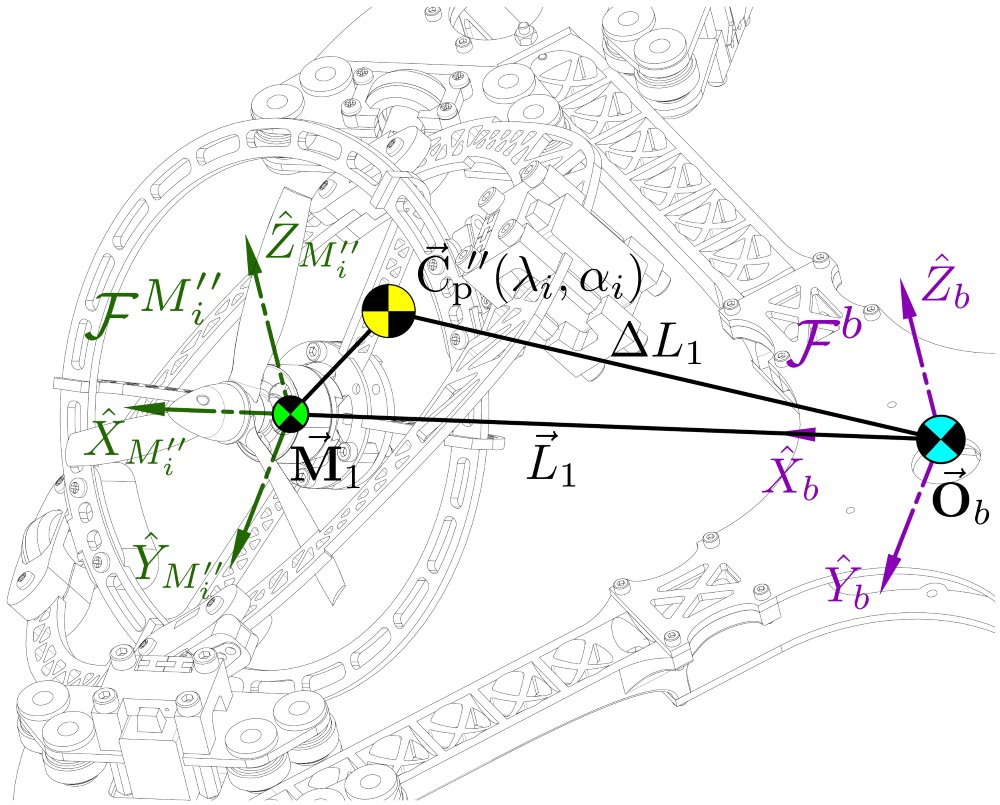
\includegraphics[width=0.55\textwidth]{figs/vector-diff}
\caption{Illustration of rotated center of gravity $C.M_\text{p}'$}
\label{fig:vector-diff}
\vspace{-20pt}
\end{figure}
\par
The time derivative of that module's moving center of gravity, $C.M_\text{p}'$ relative to the origin $\vec{\mathbf{O}}_b$, is:
\begin{equation}
\Delta \dot{L}_i=-\frac{d}{dt}\Big(C.M_\text{p}'\Big)
\end{equation}
\vspace{-10pt}
\begin{equation}
=-\frac{1}{m_\text{p}}\Big(m_\text{n}\big(R_z\big([\dot{\vec{\alpha}}_i]_\times R_y(\alpha)R_x(\lambda)C.M_\text{n}+R_y(\alpha)[\dot{\vec{\lambda}}_i]_\times C.M_\text{n}\big)+m_\text{m}R_z[\dot{\vec{\alpha}}_i]_\times C.M_\text{m}\Big)
\end{equation}
\end{subequations}
Then, extended from Lemma:\ref{lem:1}, the motor module's \emph{point-mass} inertia $J_H$ about the origin $\vec{\mathbf{O}}_b$ is defined, with motor module mass $m_\text{p}=m_\text{n}+m_\text{m}$, using masses $m_\text{n}$ and $m_\text{m}$ from Eq:\ref{eq:body-net-inner.a} and Eq:\ref{eq:body-net-middle.a}:
\begin{subequations}
\begin{equation}\label{eq:module-point-mass}
J_H\triangleq m_\text{p}\Big(\big(\Delta L_i \cdot \Delta L_i\big)\mathbb{I}_{3\times 3}-\Delta L_i \otimes \Delta L_i\Big)
\end{equation}
Or, using the definition of inner and outer products:
\begin{equation}
=m_\text{p}\Big(\big[\Delta L_i\big]^T\big[\Delta L_i\big]-\big[\Delta L_i\big]\big[\Delta L_i\big]^T\Big)
\end{equation}
Which leads to the that point mass's inertial rate $d/dt\big({J}_H\big)$:
\begin{equation}\label{eq:module-point-mass-rate}
\dot{J}_H=m_\text{p}\Big(\big[\Delta \dot{L}_i\big]^T\big[\Delta L_i\big]+\big[\Delta L_i\big]^T\big[\Delta \dot{L}_i\big]-\big[\Delta \dot{L}_i\big]\big[\Delta L_i\big]^T-\big[\Delta L_i\big]\big[\Delta \dot{L}_i\big]^T\Big)
\end{equation}
\end{subequations}
Unfortunately that inertial rate, $\dot{J}_H$ in Eq:\ref{eq:module-point-mass-rate}, cannot be simplified further to a more concise form. The Lagrangian for the energy of a single motor module, about the origin $\vec{\mathbf{O}}_b$, $\mathcal{L}_{p_i}$ can then be constructed. This time, \emph{including} the gravitational potential energy component:
\begin{multline}
\mathcal{L}_{p_i}=\frac{1}{2}\vec{\omega}_{r/I}^T\big(J_r'''\big)\vec{\omega}_{r/I}+\frac{1}{2}\vec{\omega}_{M_i/I}^T\big(J_{ir}'''\big)\vec{\omega}_{M_i/I}+\frac{1}{2}\vec{\omega}_{M_i'/I}^T\big(J_m''\big)\vec{\omega}_{M_i'/I}+\vec{\omega}_{b/I}^T\big(J_H)\vec{\omega}_{b/I}\\-m_p\vec{G}_b\cdot\big(R_I^b(\eta)\vec{\mathcal{E}}+\Delta L_i\big)
\end{multline}
Where the term $m_b\vec{G}_b\cdot\big(R_I^b(\eta)\vec{\mathcal{E}}+\Delta L_i\big)$ is the vector analogue of gravitational potential energy $m\vec{g}h$ with $R_I^b(\eta)\vec{\mathcal{E}}$ being the relative X-Y-Z inertial frame position in the body frame $\mathcal{F}^b$ relative to the body origin $\vec{\mathbf{O}}_b$. Expanding $\mathcal{L}_{p_i}$ with terms defined previously:
\begin{multline}
\rightarrow\mathcal{L}_{p_i}=\Big[\vec{\Omega}_i'''+\dot{\vec{\lambda}}_i''+\dot{\vec{\alpha}}_i'+\vec{\omega}_b\Big]^T\big(J_r'''\big)\Big[\vec{\Omega}_i'''+\dot{\vec{\lambda}}_i''+\dot{\vec{\alpha}}_i+\vec{\omega}_b\Big]+\Big[\dot{\vec{\lambda}}_i''+\dot{\vec{\alpha}}_i'+\vec{\omega}_b\Big]^T\big(J_{ir}'''\big)\Big[\dot{\vec{\lambda}}_i''+\dot{\vec{\alpha}}_i'+\vec{\omega}_b\Big]
\\
\Big[\dot{\vec{\alpha}}_i'+\vec{\omega}_b\Big]^T\big(J_m''\big)\Big[\dot{\vec{\alpha}}_i'+\vec{\omega}_b\Big]+\vec{\omega}_{b}^T\big(m_p\Big(\big[\Delta L_i\big]^T\big[\Delta L_i\big]-\big[\Delta L_i\big]\big[\Delta L_i\big]^T\Big)\big)\vec{\omega}_{b}
\\
-m_p\vec{G}_b\cdot\big(R_I^b(\eta)\vec{\mathcal{E}}+\Delta L_i\big)
\end{multline}
Applying partial derivatives of the Lagrangian formulation to $\mathcal{L}_{p_i}$ relative to the angular path co-ordinates $\vec{\eta}_b$ and $\vec{\omega}_b$ to find generalized forced $\vec{\mathbf{W}}$. Recalling $\vec{\eta}_b$ is the angular orientation from Eq:\ref{eq:angular-rates.b}, defined entirely in the body frame $\mathcal{F}^b$, and similarly assuming that $\partial/\partial\vec{\eta}_b\big(\Delta L_i\big)\approx 0$:
\begin{subequations}
\begin{equation}\label{eq:lagrange-module-body}
\frac{d}{dt}\bigg(\frac{\partial\mathcal{L}_{p_i}}{\partial\dot{\vec{\eta}}_b}\bigg)-\frac{\partial\mathcal{L}_{p_i}}{\partial\vec{\eta}_b}=\frac{d}{dt}\bigg(\frac{\partial\mathcal{L}_{p_i}}{\partial\vec{\omega}_b}\bigg)-\frac{\partial\mathcal{L}_{p_i}}{\partial\vec{\eta}_b}=\vec{\mathbf{W}}=\vec{\tau}_M
\end{equation}
\vspace{-14pt}
\begin{multline}
=\frac{d}{dt}\bigg(\big(J_r'''\big)\Big[\vec{\Omega}_i'''+\dot{\vec{\lambda}}_i''+\dot{\vec{\alpha}}_i'+\vec{\omega}_b\Big]+\big(J_{ir}'''\big)\Big[\dot{\vec{\lambda}}_i''+\dot{\vec{\alpha}}_i'+\vec{\omega}_b\Big]+\big(J_m''\big)\Big[\dot{\vec{\alpha}}_i'+\vec{\omega}_b\Big]+\big(J_H\big)\Big[\vec{\omega}_b\Big]\bigg)
\\
+m_p\vec{G}_b\times\Delta{L}_i
\end{multline}
Then using inertial rate derivatives from Eq:\ref{eq:body-rotor-rate}-\ref{eq:body-middle-rate} and $\dot{J}_H$ from Eq:\ref{eq:module-point-mass-rate}, and inserting relative angular velocities from Eq:\ref{eq:body-rotor-angular}-\ref{eq:body-middle-angular}:
\begin{multline}
=\Big[\big(\dot{J}_r'''\big)(\vec{\Omega}_i'''+\dot{\vec{\lambda}}_i''+\dot{\vec{\alpha}}_i'+\vec{\omega}_b)\Big]+\Big[\big(J_r'''\big)\dot{\vec{\Omega}}_i'''+\vec{\omega}_{M_i/I}\times\big(J_r'''\big)\vec{\Omega}_i'''+\big(J_r'''\big)\ddot{\vec{\lambda}}_i''+\vec{\omega}_{M_i/I}\times \big(J_r'''\big)\dot{\vec{\lambda}}_i''
\\
+\big(J_r'''\big)\ddot{\vec{\alpha}}_i'+\vec{\omega}_{M_i'/I}\times\big(J_r'''\big)\dot{\vec{\alpha}}_i'+\big(J_r'''\big)\dot{\vec{\omega}}_b+\vec{\omega}_{b/I}\times\big(J_r'''\big)\vec{\omega}_b\Big]+\Big[\big(\dot{J}_{ir}'''\big)(\dot{\vec{\lambda}}_i''+\dot{\vec{\alpha}}_i'+\vec{\omega}_b)\Big]+\Big[\big(J_{ir}'''\big)\ddot{\vec{\lambda}}_i''
\\
+\vec{\omega}_{M_i/I}\times\big(J_{ir}'''\big)\dot{\vec{\lambda}}_i''+\big(J_{ir}'''\big)\ddot{\vec{\alpha}}_i'+\vec{\omega}_{M_i'/I}\times\big(J_{ir}'''\big)\dot{\vec{\alpha}}_i'+\big(J_{ir}'''\big)\dot{\vec{\omega}}_b+\vec{\omega}_{b/I}\times\big(J_{ir}'''\big)\vec{\omega}_b\Big]+\Big[\big(\dot{J}_m''\big)(\dot{\vec{\alpha}}_i'+\vec{\omega}_b)\Big]
\\
\Big[\big(J_m''\big)\ddot{\vec{\alpha}}_i'+\vec{\omega}_{M_i'/I}\times\big(J_m''\big)\dot{\vec{\alpha}}_i'+\big(J_m''\big)\dot{\vec{\omega}}_b+\vec{\omega}_{b/I}\times\big(J_m''\big)\vec{\omega}_b\Big]+\Big[\big(\dot{J}_h\big)\vec{\omega}_b\Big]+\Big[\big(J_H\big)\dot{\vec{\omega}}_b+\vec{\omega}_{b/I}\times\big(J_h\big)\vec{\omega}_b\Big]
\\
+\Big[m_p\vec{G}_b\times\Delta L_i\Big]
\end{multline}
After expanding relative angular velocity terms; $\vec{\omega}_{M_i/I}$, $\vec{\omega}_{M_i'/I}$, $\vec{\omega}_{M_i''/I}$ and $\vec{\omega}_{b/I}$ and applying some mathematics, Eq:\ref{eq:lagrange-module-body} is shown to include a transformed component of Eq:\ref{eq:alpha-lagrange-deriv}.
\begin{multline}
\rightarrow\frac{d}{dt}\bigg(\frac{\partial\mathcal{L}_{p_i}}{\partial\vec{\omega}_b}\bigg)-\frac{\partial\mathcal{L}_{p_i}}{\partial\vec{\eta}_b}=R_z\frac{d}{dt}\bigg(\frac{\partial\mathcal{L}_{M_i''}}{\partial\dot{\vec{\mathbf{v}}}}\bigg)+\big(\dot{J}_r'''\big)\vec{\omega}_b+\vec{\omega}_b\times\big(J_r'''\big)\vec{\Omega}_i'''+\vec{\omega}_b\times\big(J_r'''\big)\dot{\vec{\lambda}}_i''+\vec{\omega}_b\times\big(J_r'''\big)\dot{\vec{\alpha}}_i'
\\
+\vec{\omega}_b\times\big(J_r'''\big)\vec{\omega}_b+J_r'''\dot{\vec{\omega}}_b+\big(\dot{J}_{ir}'''\big)\vec{\omega}_b+\vec{\omega}_b\times\big(J_{ir}'''\big)\dot{\vec{\lambda}}_i''+\vec{\omega}_b\times\big(J_{ir}'''\big)\dot{\vec{\alpha}}_i'+\vec{\omega}_b\times\big(J_{ir}'''\big)\vec{\omega}_b+\big(J_{ir}'''\big)\dot{\vec{\omega}}_b
\\
\big(\dot{J}_m''\big)\vec{\omega}_b+\vec{\omega}_b\times\big(J_m''\big)\dot{\vec{\alpha}}_i'+\vec{\omega}_b\times\big(J_m''\big)\vec{\omega}_b+\big(J_m''\big)\dot{\vec{\omega}}_b+\big(\dot{J}_H\big)\vec{\omega}_b+\big(J_H\big)\dot{\vec{\omega}}_b+\vec{\omega}_b\times\big(J_H\big)\vec{\omega}_b
\\
+m_p\vec{G}_b\times\Delta{L}_i
\end{multline}
Combining inertial bodies with the same angular velocities and introducing terms $\vec{\tau}_\lambda$ and $\vec{\tau}_\alpha$ from Eq:\ref{eq:torque-induced-inner} and Eq:\ref{eq:torque-induced-middle} respectively:
\begin{multline}\label{eq:module-forces-w}
\therefore\vec{\mathbf{W}}=\vec{\tau}_M=R_z\vec{\tau}_\alpha(\lambda)+R_zR_y(\alpha)\vec{\tau}_\lambda + \big(\dot{J}_r'''+\dot{J}_{ir}'''+\dot{J}_m''+\dot{J}_H\big)\vec{\omega}_b+\big(J_r'''+J_{ir}'''+J_m'+J_H\big)\dot{\vec{\omega}}_b
\\
+\vec{\omega}_b\times\big(J_r'''+J_{ir}'''+J_m''+J_H\big)\vec{\omega}_b+\vec{\omega}_b\times\Big(\big(J_r'''\big)(\vec{\omega}_i'''+\dot{\vec{\lambda}}_i''+\dot{\vec{\alpha}}_i')+\big(J_{ir}'''\big)(\dot{\vec{\lambda}}_i''+\dot{\vec{\alpha}}_i')+\big(J_m''\big)(\dot{\vec{\alpha}}_i')\Big)
\\
+m_p\vec{G}_b\times\Delta{L}_i
\end{multline}
\end{subequations}
And recognizing that $(J_r'''+J_{ir}'''+J_m''+J_H)$ can be simplified to a parallel axis translation of the transformed net motor module inertia $J_p'$ from Eq:\ref{eq:inertia.middle.b}; analogous to the net motor module inertia defined in Eq:\ref{eq:body-inertia.b}:
\begin{subequations}
\begin{multline}
(J_r'''+J_{ir}'''+J_m''+J_H)=R_zR_y(\alpha)R_x(\lambda)\big(J_r\big)R_x^{-1}(\lambda)R_y^{-1}(\alpha)R_z^{-1}
\\
+R_zR_y(\alpha)R_x(\lambda)\big(J_{ir}\big)R_x^{-1}(\lambda)R_y^{-1}(\alpha)R_z^{-1}+R_zR_y(\alpha)\big(J_m\big)R_y^{-1}(\alpha)R_z^{-1}+J_H
\end{multline}
\vspace{-12pt}
\begin{equation}
=R_z\big(J_p\big)R_z^{-1}+m_p\Big(\big[\Delta L_i\big]^T\big[\Delta L_i\big]-\big[\Delta L_i\big]\big[\Delta L_i\big]^T\Big)=J_{\vec{\mathbf{M}}_i}'
\end{equation}
Moreover, the above can be applied to the associated inertia rates $\dot{J}_r'''$, $\dot{J}_{ir}'''$, $\dot{J}_m''$ and $\dot{J}_H$. Using Eq:\ref{eq:body-rotor-rate},\ref{eq:body-inner-rate},\ref{eq:body-middle-rate} and \ref{eq:module-point-mass-rate} it can be shown that:
\begin{equation}\label{eq:module-inertia-rates}
\big(\dot{J}_r'''+\dot{J}_{ir}'''+\dot{J}_m''+\dot{J}_H\big)=\dot{J}_{\vec{\mathbf{M}}_i}'
\end{equation}
\end{subequations}
The generalized torque acting on a single motor module, $\vec{\tau}_M$ from Eq:\ref{eq:module-forces-w}, is then found as combinations of responses to servos $\lambda_i$ and $\alpha_i$, the changing inertial rates $\dot{J}_{\vec{\mathbf{M}}_i}'$ as a result of those rotations and finally the net response to the entire frames angular velocity $\vec{\omega}_b$.
\begin{multline}\label{eq:module-response}
\vec{\tau}_M=R_z\vec{\tau}_\alpha(\lambda)+R_zR_y(\alpha)\vec{\tau}_\lambda+\big(\dot{J}_{\vec{\mathbf{M}}_i}'\big)\vec{\omega}_b+\big(J_{\vec{\mathbf{M}}_i}'\big)\dot{\vec{\omega}}_b+\vec{\omega}_b\times\big(J_{\vec{\mathbf{M}}_i}'\big)\vec{\omega}_b
\\
+\vec{\omega}_b\times\Big(\big(J_p''\big)\dot{\vec{\alpha}}_i'+\big(J_n'''\big)\dot{\vec{\lambda}}_i''+\big(J_r'''\big)\vec{\Omega}_i'''\Big)+m_p\vec{G}_b\times\Delta{L}_i~~~~\in\mathcal{F}^b
\end{multline}
Considering the rigid body response for the body structure's motion, $J_y$. That structure's inertia $J_y$ is a constant which represents the vehicle's constant, rigid inertias which are not included in the motor module; defined previously in Eq:\ref{eq:inertia.body.c}.
\begin{equation}\label{eq:structure-response}
\vec{\tau}_y=\big(J_y\big)\dot{\vec{\omega}}_b+\vec{\omega}_b\times\big(J_y\big)\vec{\omega}_b~~~~\in\mathcal{F}^b
\end{equation}
The net response for the \emph{entire} multibody system is then a sum of Eq:\ref{eq:module-response} for modules $i\in[1:4]$ and $\vec{\tau}_y$ in Eq:\ref{eq:structure-response}. By inspection, without constructing a complete Lagrangian for the entire system, the net torque acting on the body frame $\mathcal{F}^b$ is:
\begin{equation}\label{eq:3.85}
\vec{\tau}_\mu = \big(J_y\big)\dot{\vec{\omega}}_b+\vec{\omega}_b\times\big(J_y\big)\vec{\omega}_b+\sum_{i=1}^{4}\vec{\tau}_{M}(i)~~~~\in\mathcal{F}^b
\end{equation}
Recalling the net vehicles rotational inertia $J_b(u)$, calculated as a function of the actuation matrix $u$, which was defined previously in \ref{eq:body-net-2}. It follows that Eq:\ref{eq:3.85} reduces to:
\begin{multline}
\vec{\tau}_\mu=\big(J_b(u)\big)\dot{\vec{\omega}}_b+\vec{\omega}_b\times\big(J_b(u)\big)\vec{\omega}_b
\\
-\sum_{i=1}^{4}\Big[R_z\vec{\tau}_\alpha(\lambda)+R_zR_y(\alpha)\vec{\tau}_\lambda+\big(\dot{J}_{\vec{\mathbf{M}}_i}\big)\vec{\omega}_b+\vec{\omega}_b\times\Big(\big(J_p''\big)\dot{\vec{\alpha}}_i'+\big(J_n'''\big)\dot{\vec{\lambda}}_i''+\big(J_r'''\big)\vec{\Omega}_i'''\Big)\Big]
\\
-m_p\vec{G}_b\times\sum_{i=1}^{4}\Delta L_i
\end{multline}
The final sum of gravitational torque arms can be reduced to $\vec{\tau}_g$ from Eq:\ref{eq:grav-torque} which considers the \emph{net} resultant center of gravity. Then, extending the angular differential equation Eq:\ref{eq:states.d} to incorporate the multibody responses derived above:
\begin{subequations}
\begin{equation}\label{eq:3.110a}
\vec{\tau}_\mu=\big(J_b\big)\dot{\vec{\omega}}_b+\vec{\omega}_b\times\big(J_b\big)\vec{\omega}_b-\vec{\tau}_b-\vec{\tau}_g
\end{equation}
Using the net gravitational torque arm $\vec{\tau}_g$ defined earlier in Eq:\ref{eq:grav-torque}:
\begin{equation}\label{eq:net-body-gravity}
\vec{\tau}_g\triangleq\Delta C.G\times m_b\vec{G}_b
\end{equation}
And defining a new response torque $\vec{\tau}_b$ which represents collective responses from internal rotations relative each body, $i^{\text{th}}$ arguments for motor modules are implied:
\begin{equation}\label{eq:net-body-response}
\vec{\tau}_b\triangleq\dot{J}_b(u)\vec{\omega}_b+\sum_{i=1}^{4}\Big[R_z\vec{\tau}_\alpha(\lambda)+R_zR_y(\alpha)\vec{\tau}_\lambda+\vec{\omega}_b\times\Big(\big(J_p''\big)\dot{\vec{\alpha}}_i'+\big(J_n'''\big)\dot{\vec{\lambda}}_i''+\big(J_r'''\big)\vec{\Omega}_i'''\Big)\Big]
\end{equation}
\end{subequations}
Noting that $\dot{J}_b(u)$ is another introduced term which is the sum of all module inertia rates from Eq:\ref{eq:module-inertia-rates}, given that body structures inertia $J_y$ is constant:
\begin{equation}
\dot{J}_b(u)\triangleq \sum_{i=1}^4 \big(\dot{J}_{\vec{\mathbf{M}}_i}'\big)
\end{equation}
The torque $\vec{\tau}_b$ in Eq:\ref{eq:net-body-response} is the most important result here, however; definitions of $\vec{\tau}_\alpha(\lambda)$ and $\vec{\tau}_\lambda$ in Eq:\ref{eq:torque-induced-inner} and Eq:\ref{eq:torque-induced-middle} respectively were necessary to simplify and isolate different components of Eq:\ref{eq:net-body-response}. Depending on the magnitude of $\dot{\lambda}_i$ and $\dot{\alpha}_i$; $\vec{\tau}_b$ could be further simplified to an approximation $\hat{\tau}_b$:
\begin{equation}\label{eq:net-body-approx}
\hat{\tau}_b\triangleq\dot{J}_b(u)\vec{\omega}_b\approx\vec{\tau}_b\Big|_{\alpha,\lambda<<1}
\end{equation}
\begin{figure}[hbtp]
\vspace{-6pt}
\centering
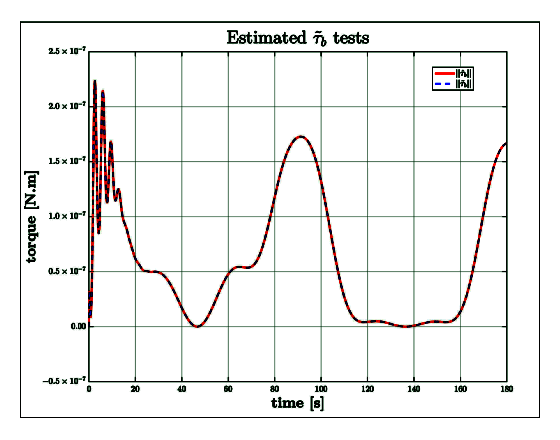
\includegraphics[width=0.45\textwidth]{graphs/tau-body}
\caption{Approximated and true body torque responses}
\vspace{-12pt}
\label{fig:tau-body}
\vspace{-6pt}
\end{figure}
\par
Moreover, that inertial rate for $\dot{J}_b$ could be further approximated simply as the difference of instantaneous calculations for $J_b(u)$ at some sample time $n$; if a constant sample rate or time difference $\Delta t$ is known:
\begin{equation}
\dot{J}_b(u)\approx \big(J_b(u_n)-J_b(u_{n-1})\big)/\Delta t
\end{equation}
The difference between an approximated torque $\hat{\tau}_b$ and the true body torque $\vec{\tau}_b$ for a typical flight envelope is plotted in Fig:\ref{fig:tau-body}. Using Eq:\ref{eq:net-body-approx} and Eq:\ref{eq:net-body-response} respectively for $\hat{\tau}_b$ and $\vec{\tau}_b$ 
\par
Uncertainties associated with the above inertial models or their particular values can easily be compensated for as disturbances. More specifically uncertainties of the above equations system are modelled as plant dependent state uncertainties; and could be adaptively compensated for accordingly\ldots
%====================================================
\subsection{Simulation and verification of induced model}
\label{subsec:dynamics.nonlinearities.torque-tests}
%====================================================
\subsubsection{Linearization simulation and comparison}
Previously, in Sec:\ref{subsec:dynamics.nonlinearities.gyrotorques}, the proposed Lagrangian energy functions for both $\Delta\lambda$ and $\Delta\alpha$ servo rotations and responses to body angular velocities $\vec{\omega}_b$ were derived. Reiterating those energy equations; the inner ring net (kinetic) energy Lagrangian from Eq:\ref{eq:lagrange-inner} is:
\begin{subequations}
\begin{equation}\label{eq:sim-lagrange-inner}
\mathcal{L}_{M_i'}=\frac{1}{2}\vec{\omega}_{r/M_i'}\text{}^T\big(J_{r}'\big)\vec{\omega}_{r/M_i'}+\frac{1}{2}\vec{\omega}_{M_i/M_i'}\text{}^T\big(J_{ir}'\big)\vec{\omega}_{M_i/M_i'}
\end{equation}
\vspace{-16pt}
\begin{equation}\label{eq:sim-lagrange-inner-expand}
=\frac{1}{2}\Big(R_x(\lambda)\vec{\Omega}_i+\dot{\vec{\lambda}}_i\Big)^{T}\Big(R_x(\lambda)\big(J_r\big)R_x^{-1}(\lambda)\Big)\Big(R_x(\lambda)\vec{\Omega}_i+\dot{\vec{\lambda}}_i\Big)+\frac{1}{2}\big(\dot{\vec{\lambda}}_i\big)^T\Big(R_x(\lambda)\big(J_{ir}\big)R_x^{-1}(\lambda)\Big)\big(\dot{\vec{\lambda}}_i\big)
\end{equation}
And similarly for the middle ring's net (kinetic) energy from Eq:\ref{eq:alpha-lagrange}
\begin{equation}\label{eq:sim-lagrange-middle}
\mathcal{L}_{M_i''}=\frac{1}{2}\vec{\omega}_{r/M_i''}^{\hspace{2pt}T}\big(J_{r}''\big)\vec{\omega}_{r/M_i''}+\frac{1}{2}\vec{\omega}_{M_i'/M_i''}^{\hspace{2pt}T}\big(J_{ir}''\big)\vec{\omega}_{M_i'/M_i''}+\frac{1}{2}\vec{\omega}_{M_i'/M_i''}^{\hspace{2pt}T}\big(J_{m}'\big)\vec{\omega}_{M_i'/M_i''}
\end{equation}
\vspace{-20pt}
\begin{multline}\label{eq:sim-lagrange-middle-expand}
=\frac{1}{2}\Big(R_y(\alpha)R_x(\lambda)\vec{\Omega}_i+R_y(\alpha)\dot{\vec{\lambda}}_i+\dot{\vec{\lambda}}_i\Big)^T\Big(R_y(\alpha)\big(J_r'\big)R_y^{-1}(\alpha)\Big)\Big(R_y(\alpha)R_x(\lambda)\vec{\Omega}_i+R_y(\alpha)\dot{\vec{\lambda}}_i+\dot{\vec{\alpha}}_i\Big)
\\
\frac{1}{2}\Big(R_y(\alpha)\dot{\vec{\lambda}}_i+\dot{\vec{\alpha}}_i\Big)^T\Big(R_y(\alpha)\big(J_{ir}'\big)R_y^{-1}(\alpha)\Big)\Big(R_y(\alpha)\dot{\vec{\lambda}}_i+\dot{\vec{\alpha}}_i\Big)
\\
+\frac{1}{2}\Big(\dot{\vec{\alpha}}_i\Big)^T\Big(R_y(\alpha)\big(J_m\big)R_y^{-1}(\alpha)\Big)\Big(\dot{\vec{\alpha}}_i\Big)
\end{multline}
\end{subequations}
Solving for the generalized forces acting on each system requires application of Euler-Lagrange formulation, using partial derivatives relative to generalized path co-ordinates. Both the inner and middle ring systems were defined with relative co-ordinate paths for the angular servo position $\vec{\mathbf{u}}=[\lambda_i~0~0]^T$ and $\vec{\mathbf{v}}=[0~\alpha_i~0]^T$ respectively. The generalized forces for both systems are then, using the Euler-Lagrange formulation:
\begin{equation}\label{eq:sim-lagranges}
\underbrace{\frac{d}{dt}\bigg(\frac{\partial\mathcal{L}_{M_i'}}{\partial\dot{\vec{\mathbf{u}}}}\bigg)-\frac{\partial\mathcal{L}_{M_i'}}{\partial\vec{\mathbf{u}}}=\vec{\mathbf{U}}}_{\text{Inner ring}}~~\text{and}~~\underbrace{\frac{d}{dt}\bigg(\frac{\partial\mathcal{L}_{M_i''}}{\partial\dot{\vec{\mathbf{v}}}}\bigg)-\frac{\partial\mathcal{L}_{M_i''}}{\partial\vec{\mathbf{v}}}=\vec{\mathbf{V}}}_{\text{Middle ring}}
\end{equation}
The assumption in Eq:\ref{eq:rotation-linear}, presented in \cite{rotationlinearize}, is used to linearize and reduce partial derivatives of the respective inner and middle ring Lagrangians in Eq:\ref{eq:sim-lagranges}. Those simplifications are such that Eq:\ref{eq:sim-lagranges} becomes:
\begin{equation}\label{eq:sim-lagranges-linear}
\frac{d}{dt}\bigg(\frac{\partial\mathcal{L}_{M_i'}}{\partial\dot{\vec{\mathbf{u}}}}\bigg)=\vec{\mathbf{U}}~\Big|_{\big(\partial\mathcal{L}_{M_i'}/\partial\vec{\mathbf{u}}\big)\approx 0}~~\text{and}~~\frac{d}{dt}\bigg(\frac{\partial\mathcal{L}_{M_i''}}{\partial\dot{\vec{\mathbf{v}}}}\bigg)=\vec{\mathbf{V}}\Big|_{\big(\partial\mathcal{L}_{M_i''}/\partial\vec{\mathbf{v}}\big)\approx 0}
\end{equation}
Considering first the case of the inner ring Lagrangian $\mathcal{L}_{M_i'}$ in Eq:\ref{eq:sim-lagrange-inner-expand}; the partial derivative with respect to path variable $\vec{\mathbf{u}}=\vec{\lambda}_i$ was simplified:
\begin{equation}\label{eq:sim-lagrange-inner-simple}
\frac{\partial\mathcal{L}_{M_i'}}{\partial\vec{\mathbf{u}}}=\frac{\partial}{\partial\vec{\lambda}_i}\big(\mathcal{L}_{M_i'}\big)\approx 0
\end{equation}
Expanding Eq:\ref{eq:sim-lagrange-inner-simple} and finding the partial derivative of that Lagrangian, $\mathcal{L}_{M_i'}$ in Eq:\ref{eq:sim-lagrange-inner-expand}, with respect to $\vec{\mathbf{u}}=\vec{\lambda}_i$:
\begin{multline}\label{eq:3.118}
\frac{\partial\mathcal{L}_{M_i'}}{\partial\vec{\lambda}_i}=\frac{1}{2}\bigg(\frac{\partial}{\partial\vec{\lambda}_i}\Big(R_x(\lambda)\vec{\Omega}\Big)\bigg)^T\Big(R_x(\lambda)\big(J_r\big)R_x^{-1}(\lambda)\Big)\Big(R_x(\lambda)\vec{\Omega}+\dot{\vec{\lambda}}_i\Big)
\\
+\frac{1}{2}\Big(R_x(\lambda)\vec{\Omega}_i+\dot{\vec{\lambda}}_i\Big)^T\bigg(\frac{\partial}{\partial\vec{\lambda}_i}\Big(R_x(\lambda)\big(J_r\big)R_x^{-1}(\lambda)\Big)\bigg(R_x(\lambda)\vec{\Omega}_i+\dot{\vec{\lambda}}_i\Big)
\\
+\frac{1}{2}\Big(R_x(\lambda)\vec{\Omega}_i+\dot{\vec{\lambda}}_i\Big)^T\Big(R_x(\lambda)\big(J_r\big)R_x^{-1}(\lambda)\Big)\bigg(\frac{\partial}{\partial\vec{\lambda}_i}\Big(R_x(\lambda)\vec{\Omega}_i\Big)\bigg)
\\
+\frac{1}{2}\Big(\dot{\vec{\lambda}}_i\Big)^T\bigg(\frac{\partial}{\partial\vec{\lambda}_i}\Big(R_x(\lambda)\big(J_{ir}\big)R_x^{-1}(\lambda)\Big)\bigg)\Big(\dot{\vec{\lambda}}_i\Big)
\end{multline}
Testing that assumption, presented in Eq:\ref{eq:rotation-linear}; the partial derivatives in Eq:\ref{eq:3.118} are expanded upon. First considering the rotor's transformed inertia $J_r'$ with a partial derivative as per the differential product rule:
\begin{subequations}
\begin{equation}
\frac{\partial}{\partial\vec{\mathbf{u}}} J_r' = \frac{\partial}{\partial\vec{\lambda}_i}\bigg(R_x(\lambda)\big(J_r\big)R_x^{-1}(\lambda)\bigg)
\end{equation}
\vspace{-8pt}
\begin{equation}\label{eq:sim-inner-partial-rotor}
=\frac{\partial}{\partial\vec{\lambda}_i}\Big(R_x(\lambda)\Big)\big(J_r\big)R_x^{-1}(\lambda)+R_x(\lambda)\big(J_r\big)\frac{\partial}{\partial\vec{\lambda}_i}\Big(R_x^{-1}(\lambda)\Big)
\end{equation}
Similarly for the inner ring's contribution $J_{ir}'$ in Eq:\ref{eq:sim-lagrange-inner-expand}, without the rotor body's inertia:
\begin{equation}\label{eq:sim-inner-partial-inner}
\frac{\partial}{\partial\vec{\mathbf{u}}}J_{ir}'=\frac{\partial}{\partial\vec{\lambda}_i}\Big(R_x(\lambda)\Big)\big(J_{ir}\big)R_x^{-1}(\lambda)+R_x(\lambda)\big(J_{ir}\big)\frac{\partial}{\partial\vec{\lambda}_i}\Big(R_x^{-1}(\lambda)\Big)
\end{equation}
The final partial derivative to consider is that of the rotor's angular velocity $\vec{\Omega}_i$ but transformed into the inner middle ring frame $\mathcal{F}^{M_i'}$ which the Lagrangian Eq:\ref{eq:sim-lagrange-inner} is taken with respect to:
\begin{equation}\label{eq:sim-inner-partial-angular}
\frac{\partial}{\partial\vec{\lambda}_i}\Big(R_x(\lambda)\vec{\Omega}_i\Big)
\end{equation}
\end{subequations}
The application of the rotation matrix linearization, from Eq:\ref{eq:rotation-linear}, to the partial derivative rotations in Eq:\ref{eq:sim-inner-partial-rotor}-\ref{eq:sim-inner-partial-rotor} is:
\begin{subequations}
\begin{equation}\label{eq:sim-rot-linear}
R_x(\bar{\lambda}_i+\partial\lambda_i)\approx\Big(1-[\Phi_x(\bar{\lambda}_i)\partial\lambda_i]_\times\Big)R_x(\bar{\lambda}_i)
\end{equation}
Where $\Phi_x(\bar{\lambda}_i)$ is simply the partial derivative of the Euler matrix, $\Phi(\eta)$ from Eq:\ref{eq:angular-rates.f}, with respect to an $\hat{X}$ axis rotation. That being:
\begin{equation}
\Phi_x(\bar{\lambda}_i)=\begin{bmatrix}
0 & 0 & 0\\
0 & \sin{\bar{\lambda}}_i & \cos{\bar{\lambda}}_i\\
0 & -\cos{\bar{\lambda}}_i & \sin{\bar{\lambda}}_i
\end{bmatrix}
\end{equation}
So then, for some nominal $\bar{\lambda}_i$ perturbed by some small deviation $\partial\lambda_i$, Eq:\ref{eq:sim-rot-linear} expands to:
\begin{equation}
\therefore R_x(\bar{\lambda}_i+\partial\lambda_i)\approx R_x(\bar{\lambda}_i)-\begin{bmatrix}
0 & 0 & 0\\
0 & \big(c^2\bar{\lambda}_i-s^2\bar{\lambda}_i\big) & \big(-c\bar{\lambda}_is\bar{\lambda}_i-s\bar{\lambda}_ic\bar{\lambda}_i\big)\\
0 & \big(s\bar{\lambda}_ic\bar{\lambda}_i+c\bar{\lambda}_is\bar{\lambda}_i\big) & \big(c^2\bar{\lambda}_i-s^2\bar{\lambda}_i\big)
\end{bmatrix}\partial\lambda_i
\end{equation}
Which, obviously, when the perturbations $\partial\lambda_i$ away from a nominal $\bar{\lambda}_i$ are small, it follows that:
\begin{equation}
\rightarrow R_x(\bar{\lambda}_i+\partial\lambda_i)\approx R_x(\bar{\lambda}_i)\Big|_{\partial\lambda_i<<1}
\end{equation}
\end{subequations}
That simplification then applies to Eq:\ref{eq:sim-inner-partial-rotor},\ref{eq:sim-inner-partial-inner} and \ref{eq:sim-inner-partial-angular}, for a small $\partial\lambda_i$:
\begin{subequations}\label{eq:inner-ring-linearizations}
\begin{equation}
\frac{\partial}{\partial\vec{\lambda}_i}J_r'\approx 0
\end{equation}
\vspace{-8pt}
\begin{equation}
\frac{\partial}{\partial\vec{\lambda}_i}J_{ir}'\approx 0
\end{equation}
\vspace{-8pt}
\begin{equation}
\frac{\partial}{\partial\vec{\lambda}_i}R_x(\lambda)\vec{\Omega}_i\approx 0
\end{equation}
\end{subequations}
It can therefore be said that the assumption in Eq:\ref{eq:sim-lagrange-inner-simple} is not without merit, or that:
\begin{equation}
\frac{\partial\mathcal{L}_{M_i'}}{\partial\vec{\mathbf{u}}}\approx 0\rightarrow\frac{d}{dt}\bigg(\frac{\partial\mathcal{L}_{M_i'}}{\partial\dot{\vec{\mathbf{u}}}}\bigg)-\frac{\partial\mathcal{L}_{M_i'}}{\partial\vec{\mathbf{u}}}\approx\frac{d}{dt}\Big(\frac{\partial\mathcal{L}_{M_i'}}{\partial\dot{\vec{\lambda}}_i}\Big)=\vec{\mathbf{U}}=\hat{\tau}_\lambda
\end{equation}
For a final verification of those simplifications, a \textbf{Simulink} model is built that applies a direct comparison of $\vec{\tau}_\lambda$, originally from Eq:\ref{eq:torque-induced-inner}, both \emph{with} and \emph{without} the rotation matrix linearization. Convention has it that an estimated or simulated values are denoted with a hat accent. Therefore a calculated inner ring torque response \emph{with linearized} partial derivatives as per Eq:\ref{eq:inner-ring-linearizations} is termed as $\hat{\tau}_\lambda$. The true representation of the induced torque response, $\vec{\tau}_\lambda$, is calculated from the block model detailed in Fig:\ref{fig:linear-block}.
\begin{figure}[htbp]
\centering
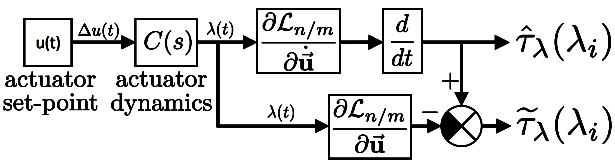
\includegraphics[width=0.6\textwidth]{figs/linear-block}
\caption{Simulink Lagrangian block}
\label{fig:linear-block}
\vspace{-15pt}
\end{figure}
\par
Where the block $u(t)$ represents some commanded change in actuator positions, $\Delta u$. That actuator change affects the actuator dynamics, grouped together here as the block $P(s)$ but detailed previously in Sec:\ref{subsec:proto.design.transfer}. That argument $u$ then leads to a servo position for $\lambda_i$ which can then be used to calculate the complete Euler-Lagrangian equation:
\begin{equation}
\frac{d}{dt}\bigg(\frac{\partial\mathcal{L}_{M_i'}}{\partial\dot{\vec{\mathbf{u}}}}\bigg)-\frac{\partial\mathcal{L}_{M_i'}}{\partial\vec{\mathbf{u}}}=\vec{\tau}_\lambda
\end{equation}
Fig:\ref{fig:tau-lambda-hat} shows plots for both estimated $\hat{\tau}_\lambda$ and simulated $\vec{\tau}_\lambda$ with a constant angular propeller speed $\vec{\Omega}_i=6500~[\text{RPM}]$. Steps up from a starting constant $\lambda(0)$ to various set points are shown in Fig:\ref{fig:tau-lambda-hat-up} whilst Fig:\ref{fig:tau-lambda-hat-down} shows steps down from various starting points to a constant $\lambda(0)$. 
\begin{figure}[hbtp]
\centering
\begin{subfigure}{0.49\textwidth}
\centering
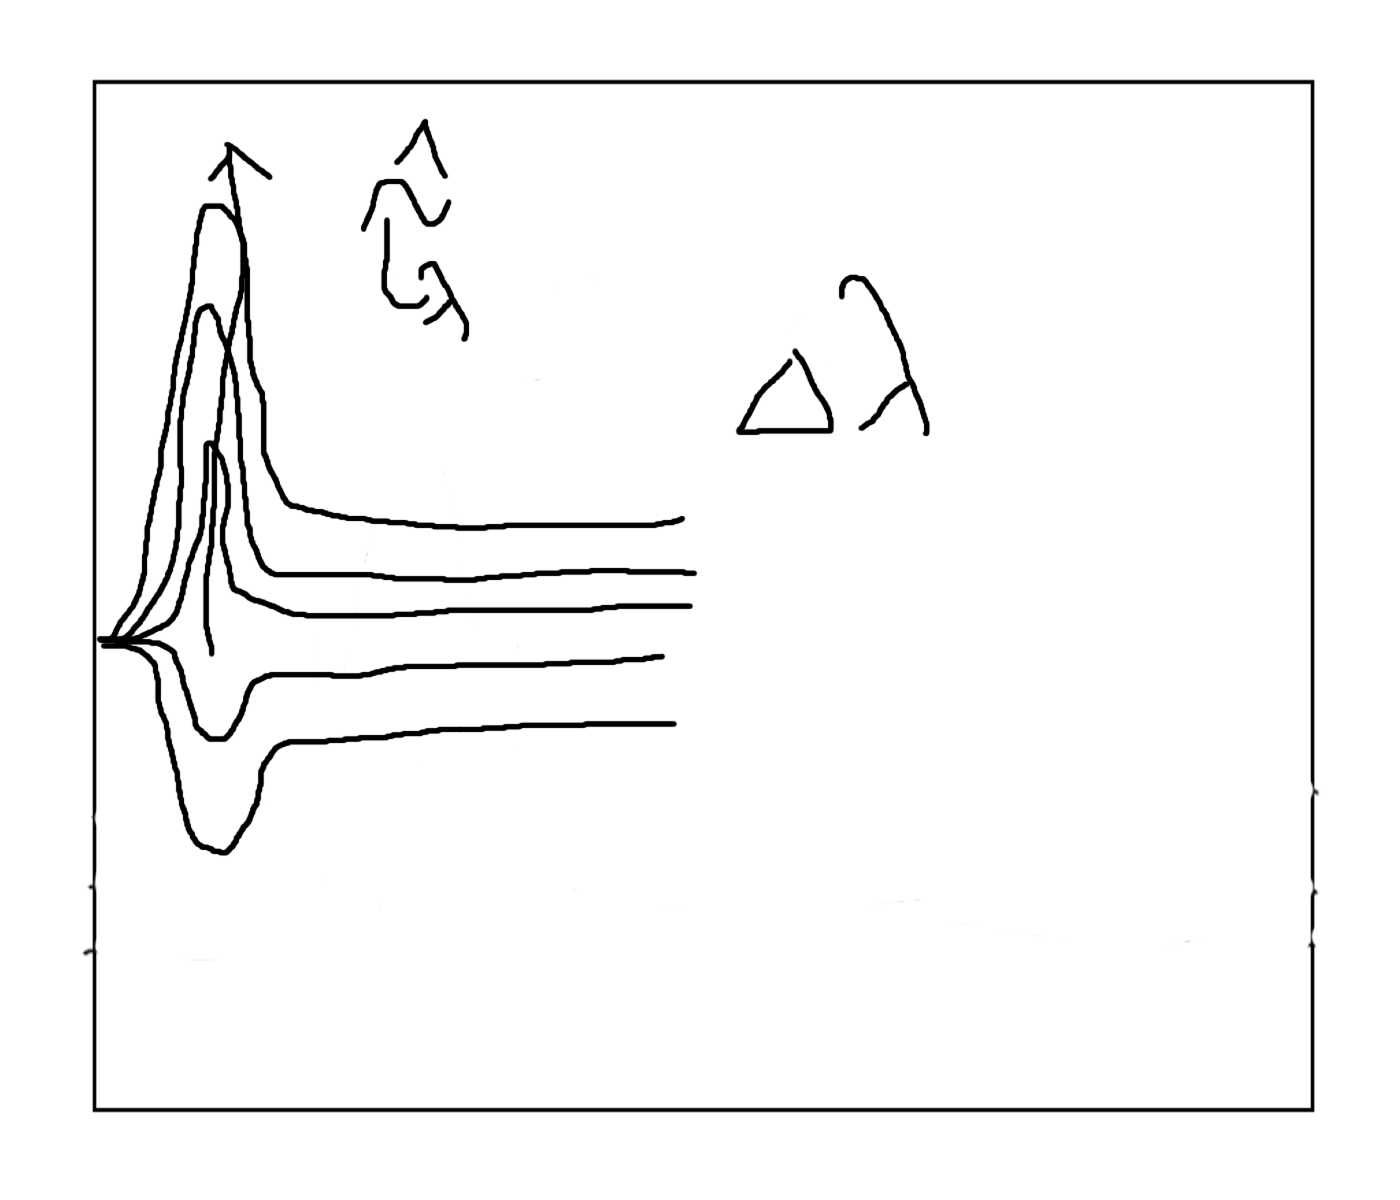
\includegraphics[width=0.95\textwidth]{graphs/tau-lambda-hat-up}
\caption{$\hat{\tau}_\lambda$ steps up}
\label{fig:tau-lambda-hat-up}
\end{subfigure}
\begin{subfigure}{0.49\textwidth}
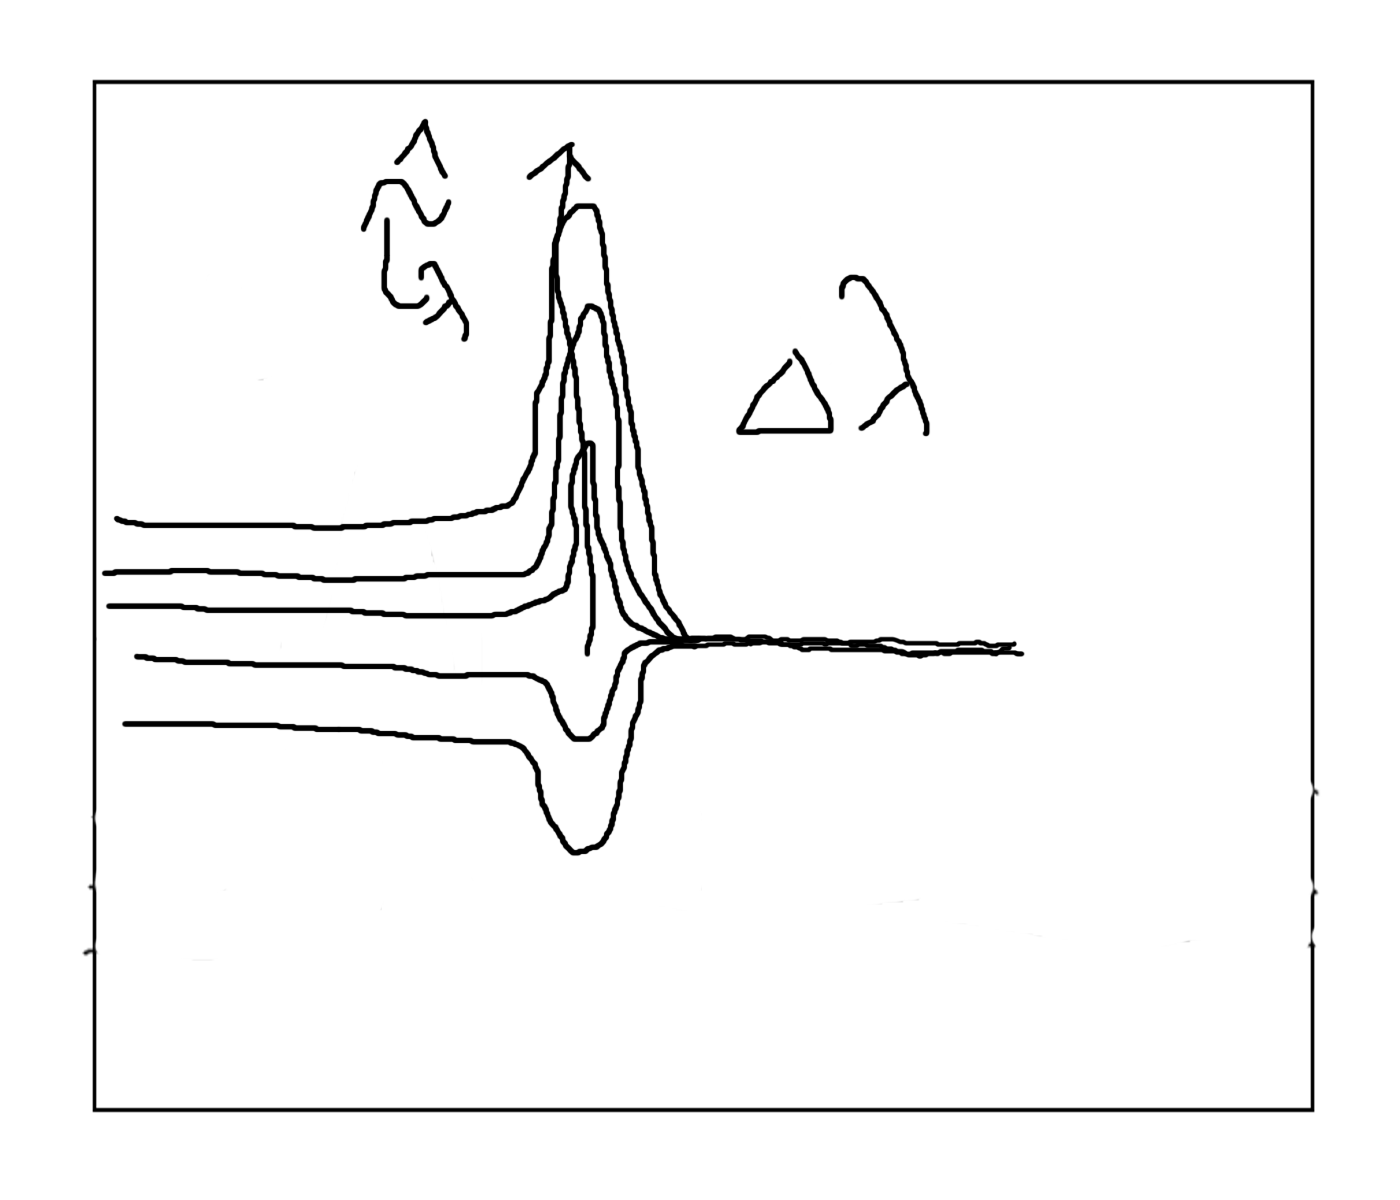
\includegraphics[width=0.95\textwidth]{graphs/tau-lambda-hat-down}
\caption{$\hat{\tau}_\lambda$ steps down}
\label{fig:tau-lambda-hat-down}
\end{subfigure}
\caption{Inner ring induced torque simulations for $\vec{\tau}_\lambda$}
\label{fig:tau-lambda-hat}
\end{figure}
\par
The difference between $\hat{\tau}_\lambda$ and $\vec{\tau}_\lambda$ is exactly the partial derivative contribution $\partial\mathcal{L}_{M_i'}/\partial\vec{\mathbf{u}}$. That difference, when using the inertial matrices and dimensions defined for the prototype in Sec:\ref{sec:proto.inertia}, is typically in the order $\times 10^{-4}~~[\text{Nm}]$ whilst both $\hat{\tau}_\lambda$ and $\vec{\tau}_\lambda$ are an order of magnitude greater than that; $\times 10^{-3}~~[\text{Nm}]$. 
\par
Following the same process applied to the middle ring Lagrangian, $\mathcal{L}_{M_i''}$ from Eq:\ref{eq:sim-lagrange-middle-expand}, yields results plotted collectively in Fig:\ref{fig:tau-alpha-hat}. The same constant propeller speed $\vec{\Omega}_i=6500~~[\text{RPM}]$ was used together with a constant $\lambda_i=\pi/5~~[\text{rad}]$ position for the inner ring's servo.
\begin{figure}[htbp]
\centering
\begin{subfigure}{0.49\textwidth}
\centering
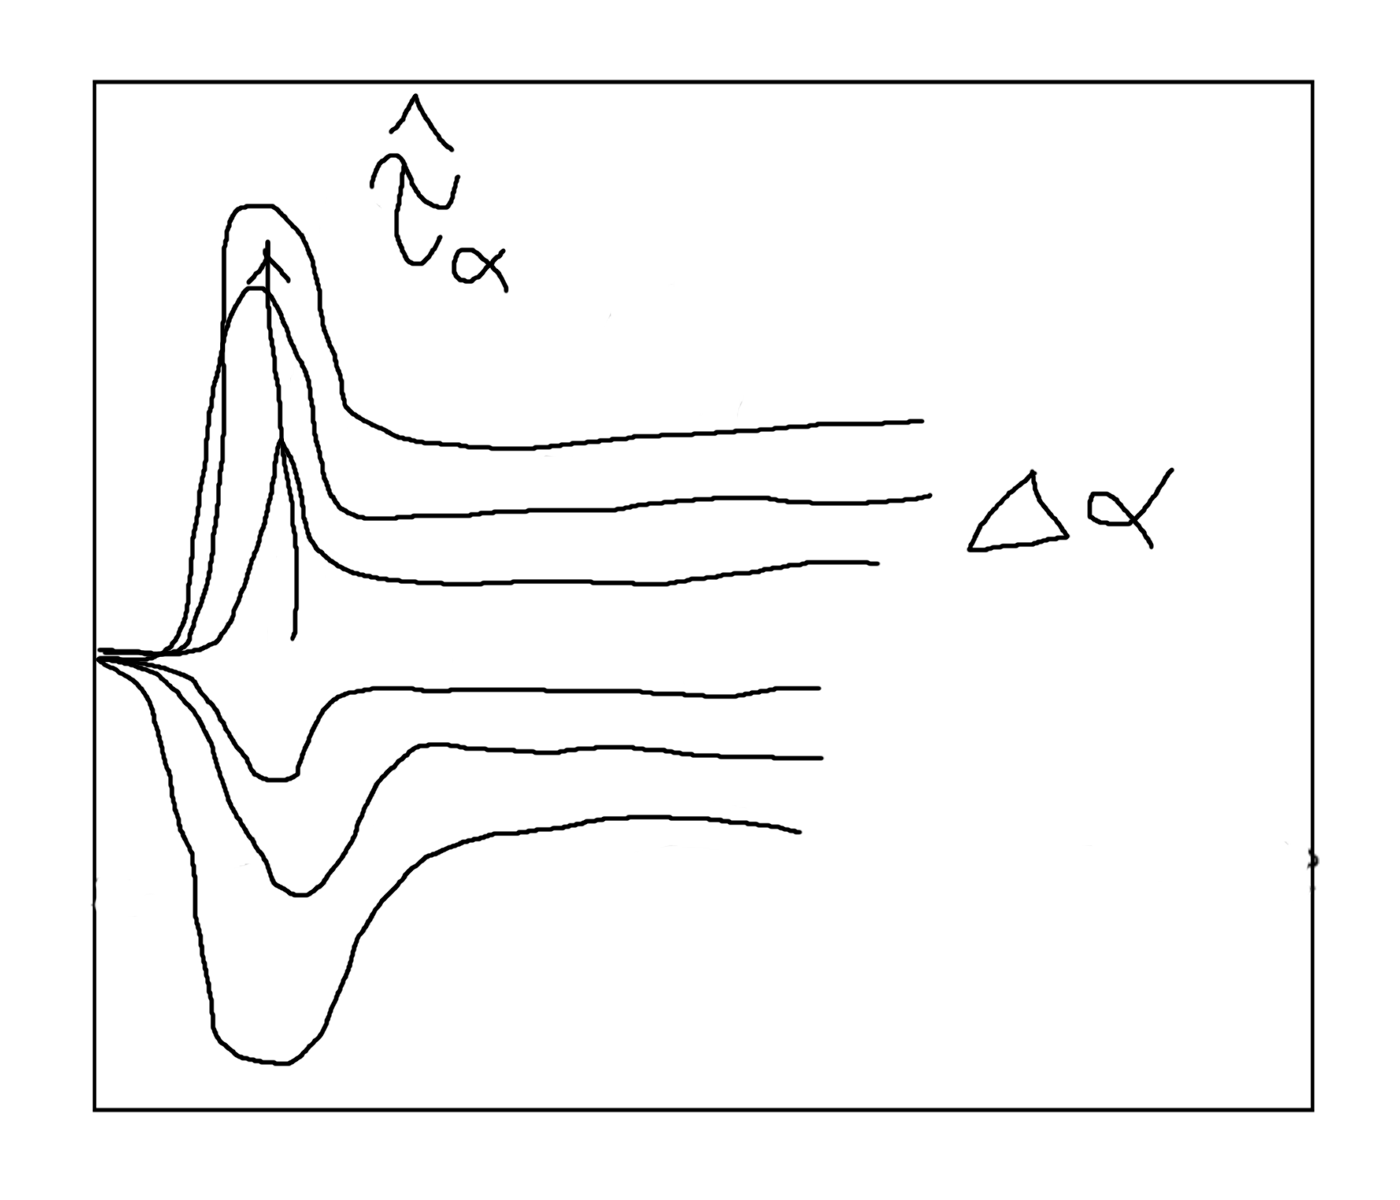
\includegraphics[width=0.95\textwidth]{graphs/tau-alpha-hat-up}
\caption{$\hat{\tau}_\alpha$ steps up}
\label{fig:tau-alpha-hat-up}
\end{subfigure}
\begin{subfigure}{0.49\textwidth}
\centering
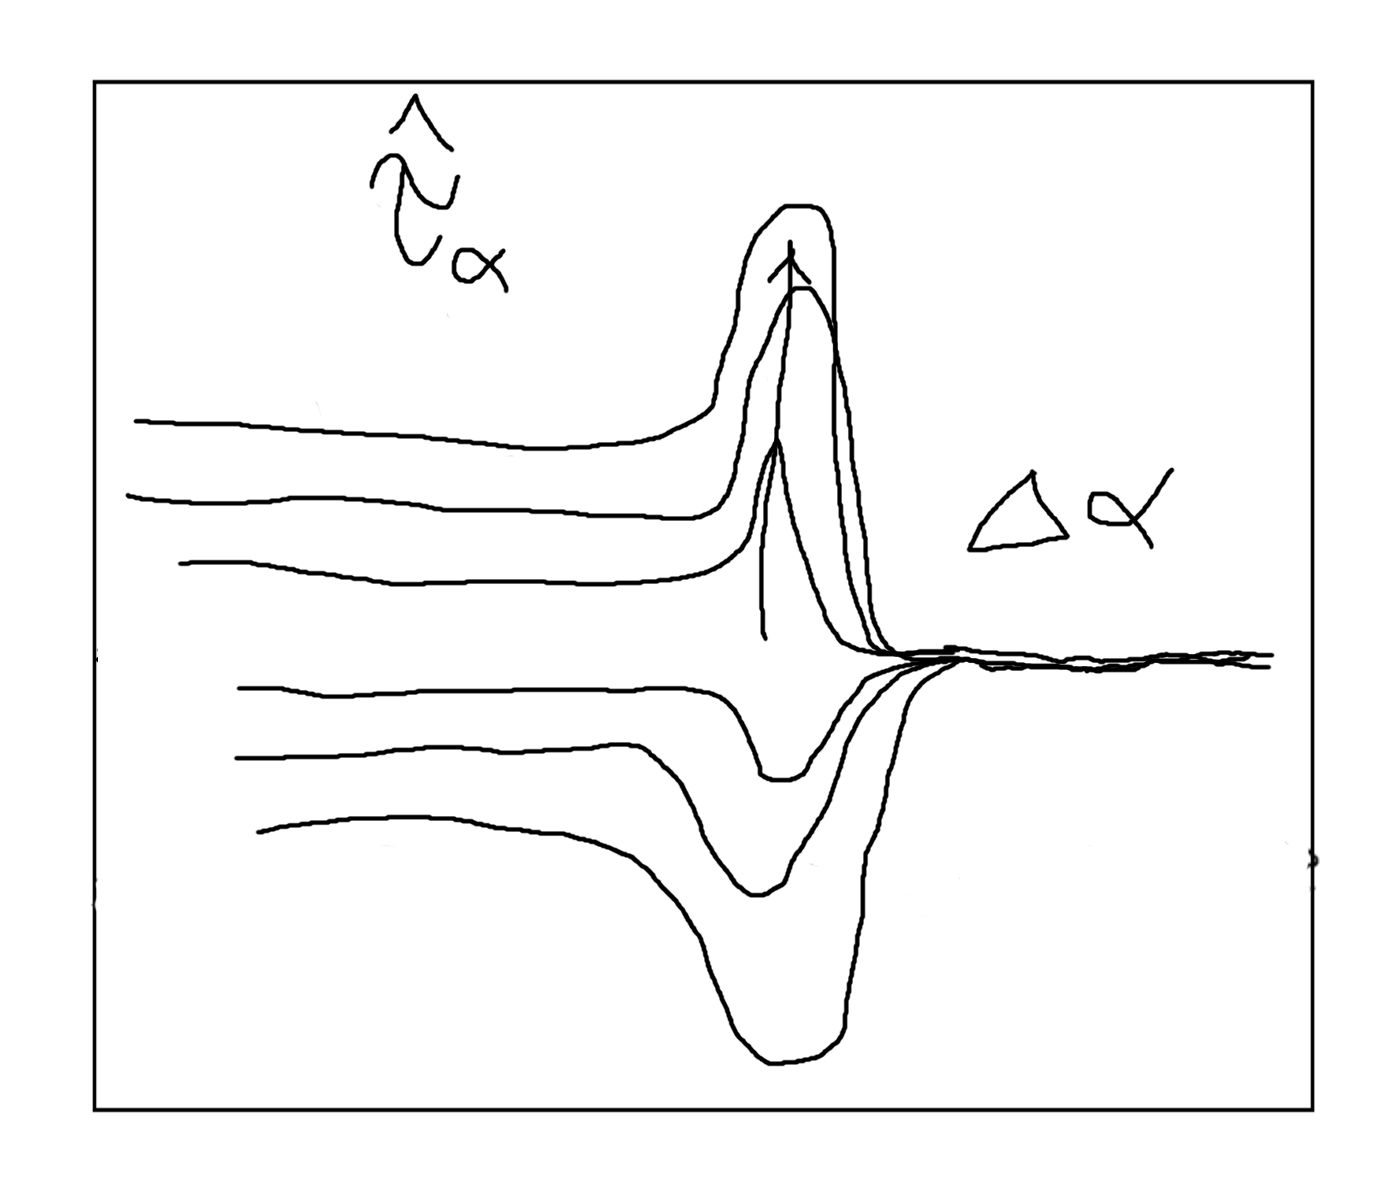
\includegraphics[width=0.95\textwidth]{graphs/tau-alpha-hat-down}
\caption{$\hat{\tau}_\alpha$ steps down}
\label{fig:tau-alpha-hat-down}
\end{subfigure}
\caption{Middle ring induced torque simulations for $\vec{\tau}_\alpha$}
\label{fig:tau-alpha-hat}
\end{figure}
\par
From plots in both Fig:\ref{fig:tau-lambda-hat} and Fig:\ref{fig:tau-alpha-hat}; it is shown that assumptions for linearizing rotation matrices in the calculations for generalized forces in Eq:\ref{eq:sim-lagranges} is not an unreasonable simplification. The linearization(s) proposed in Eq:\ref{eq:sim-lagranges-linear} hold true so long as the step size for $\Delta\lambda_i$ or $\Delta\alpha_i$ are small enough, which is always the case for the control loop. It reduces the overhead required for calculating torque responses to actuator changes. 
\subsubsection{Dynamic model verification}
In spite of the rigorous mathematics applied to the multibody system, physical corroboration of the proposed model(s) is needed. The systems described in Eq:\ref{eq:torque-induced-inner} for $\hat{\tau}_\lambda$, Eq:\ref{eq:torque-induced-middle} for $\hat{\tau}_\alpha$ and Eq:\ref{eq:torque-response} for $\hat{\tau}_b$ require further verification before a structured and accurate simulation can be constructed based upon them. 
\par
Two rigs were designed and constructed (Fig:\ref{fig:torque-inner} and Fig\ref{fig:torque-middle}) to physically measure the induced torques in question. The first test rig recreates the relative motion of the inner ring actuated by $\lambda_i$. Similarly the second test platform mimics the middle ring's motion driven by the outer $\alpha_i$ servo. The net body response, $\hat{\tau}_b$ relating to net angular body velocity $\vec{\omega}_b$, is harder to recreate on an isolated test rig. Such results are only discussed in the context of simulation and a MatLab SimScape model (see App:\ref{app:simscape}), the latter is introduced subsequently\ldots
\par
Considering first the inner most ring assembly, Fig:\ref{fig:torque-inner} shows the test rig used to isolate and measure $\vec{\tau}_\lambda$ responses to $\Delta\lambda$ rotations. The inner ring is supported by two bearing assemblies; an extended shaft in the $-\hat{X}_{M_i}$ direction connects the inner ring to the driving servo block. Rotational torque $\vec{\tau}_\lambda$ is transferred through the shaft extension from the servo to the inner ring. The servo block is secured only by a vertically aligned (and calibrated) strain gauge. The deflection of the strain gauge is then proportional to the torque applied by the servo to rotate the inner ring structure.
\newpage
\begin{figure}[htpb]
\centering
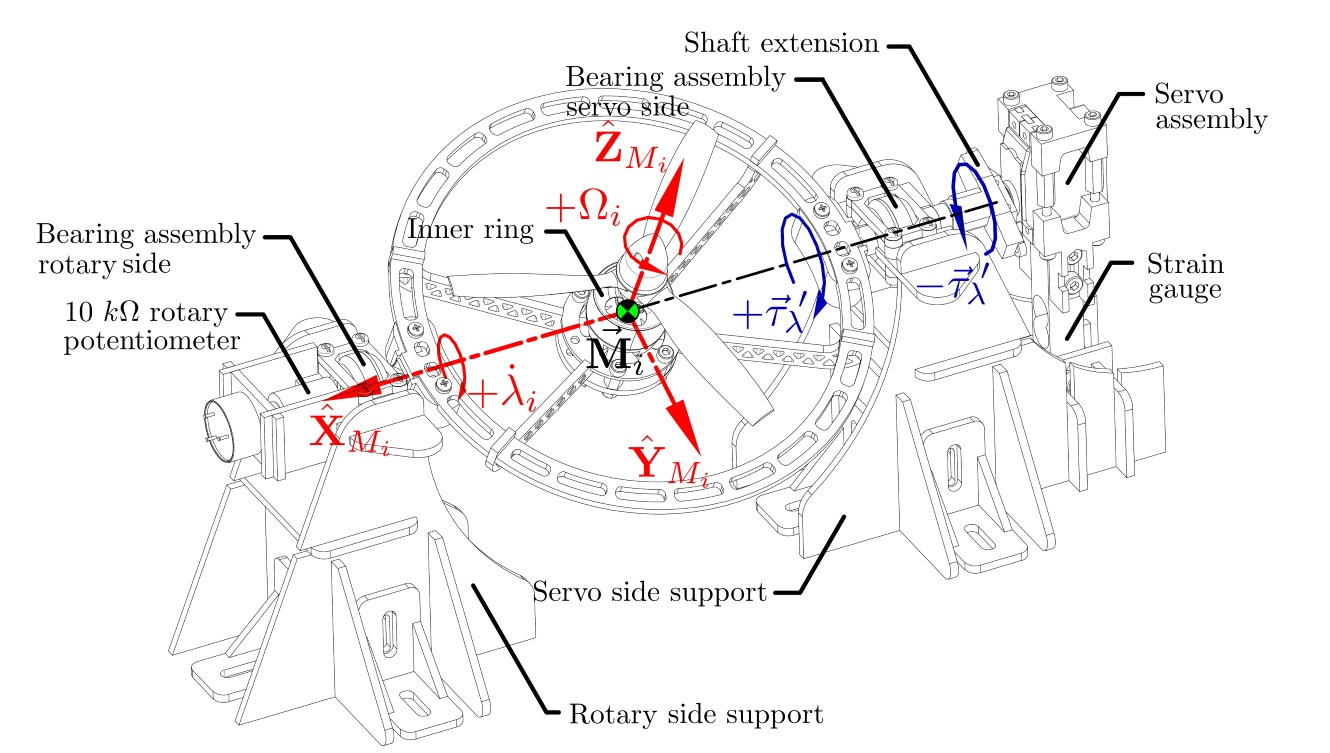
\includegraphics[width=0.8\textwidth]{figs/torque-inner}
\caption{Inner ring torque test rig}
\label{fig:torque-inner}
\vspace{-8pt}
\end{figure}
\par
It is important to mention that whilst the bearing assembly accommodates for the transfer of the servo's rotational torque, the assembly isolates only the $\hat{X}_{M_i}$ component of the induced torque. If $\vec{\tau}_{\lambda}\text{}\hspace{-2pt}'$ is the deflection measured, its relationship with the induced torque vector $\vec{\tau}_{\lambda}$ is given by:
\begin{equation}
\vec{\tau}_{\lambda}\text{}\hspace{-2pt}'=\vec{\tau}_{\lambda}\cdot\hat{X}_{M_i}~~~~\in\mathcal{F}^{M_i}
\end{equation}
One final thing to consider is that the equations for $\hat{\tau}_\lambda$ in Eq:\ref{eq:torque-induced-inner} \underline{\emph{does not}} account for the gravitational torque arm as a result of an eccentric center of gravity relative to the center of rotation. For the derivations presented previously in Sec:\ref{subsec:dynamics.nonlinearities.gyrotorques}, net gravitational torque for a resultant effective center of gravity $\vec{\tau}_g$ was later incorporated into Eq:\ref{eq:3.110a}. The torque response opposed to angular accelerations of $\ddot{\lambda}_i$ induced by the servo is then, from Eq:\ref{eq:torque-induced-inner}, with an introduced gravitational component:
\begin{multline}\label{eq:model-inner}
\vec{\tau}_\lambda=\big(\dot{J}_{r}'\big)\vec{\Omega}_i\text{}\hspace{-2pt}'+\big(\dot{J}_{n}'\big)\dot{\vec{\lambda}}_i+\big(J_r'\big)\dot{\vec{\Omega}}_i\text{}\hspace{-2pt}'+\big(J_{n}'\big)\ddot{\vec{\lambda}}_i+\dot{\vec{\lambda}}_i\times \big(J_r'\big)\vec{\Omega}_i\text{}\hspace{-2pt}'+\dot{\vec{\lambda}}_i\times \big(J_{n}'\big)\dot{\vec{\lambda}}_i
\\
+m_\text{n}C.M'_{\text{n}}\times\vec{G}_{M_i}~~~~\in\mathcal{F}^{M_i'}
\end{multline}
The term $m_\text{n}C.M'_{\text{n}}\times\vec{G}_{M_i}$ is the gravitational torque arm from a rotated center of mass, $C.M_{\text{n}}'$; first defined in Eq:\ref{eq:body-net-inner.d}. It is the effective torque contribution of a single inner ring to the net gravitational torque $\vec{\tau}_g$ from Eq:\ref{eq:net-body-gravity}. Note the strain gauge measured response encountered will be $-\hat{\tau}_\lambda$.
\par
\begin{figure}[hbtp]
\centering
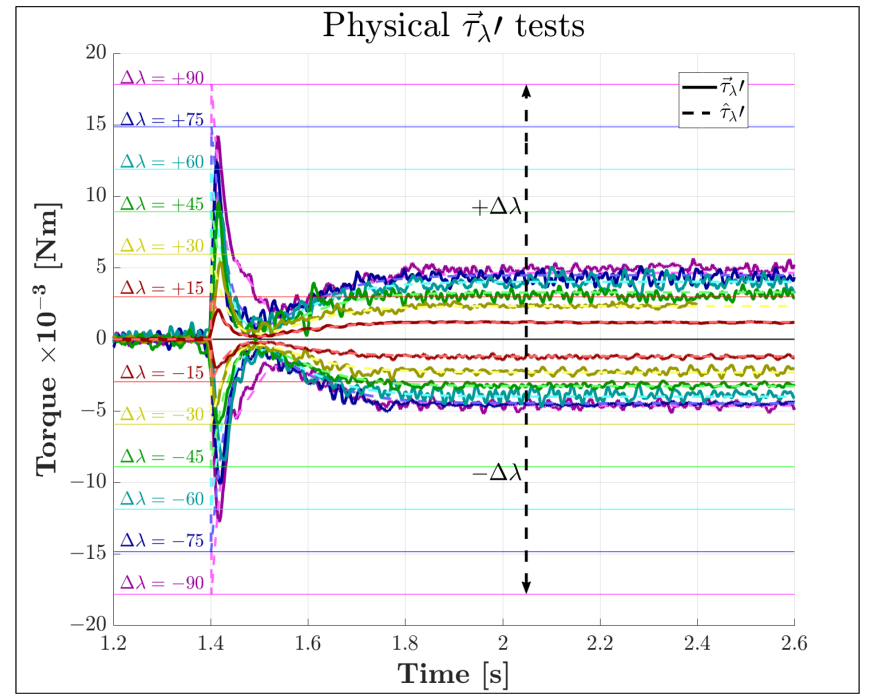
\includegraphics[width=0.55\textwidth]{graphs/tau-lambda}
\vspace{-10pt}
\caption{}
\label{fig:tau-lambda}
\vspace{-15pt}
\end{figure}
\par
The plot in Fig:\ref{fig:tau-lambda} shows simulated values of $\hat{\tau}_\lambda$ at increments of propeller rotational speeds $\Omega_i$. The torque peak changes with increased rotation rates of $\Omega_i$, motors 1 \& 3 have clockwise rotations ('+'), motors 2 \& 4 are counter-clockwise ('-'), illustrating the gyroscopic torque effect from the propeller's rotation. A postitive, clockwise rotational sense was used in the above tests. As per convention, in the plot Fig:\ref{fig:tau-lambda}, $\vec{\tau}_\lambda$ represents the physically measured torque on the test rig illustrated in Fig:\ref{fig:torque-inner}. Lastly $\tilde{\tau}_\lambda$ is a torque simulated in \textbf{MathWorks} SimScape. App:\ref{app:simscape} details how the SimScape simulation was constructed from a SolidWorks model to match the physical system.
\par
\begin{figure}[htbp]
\centering
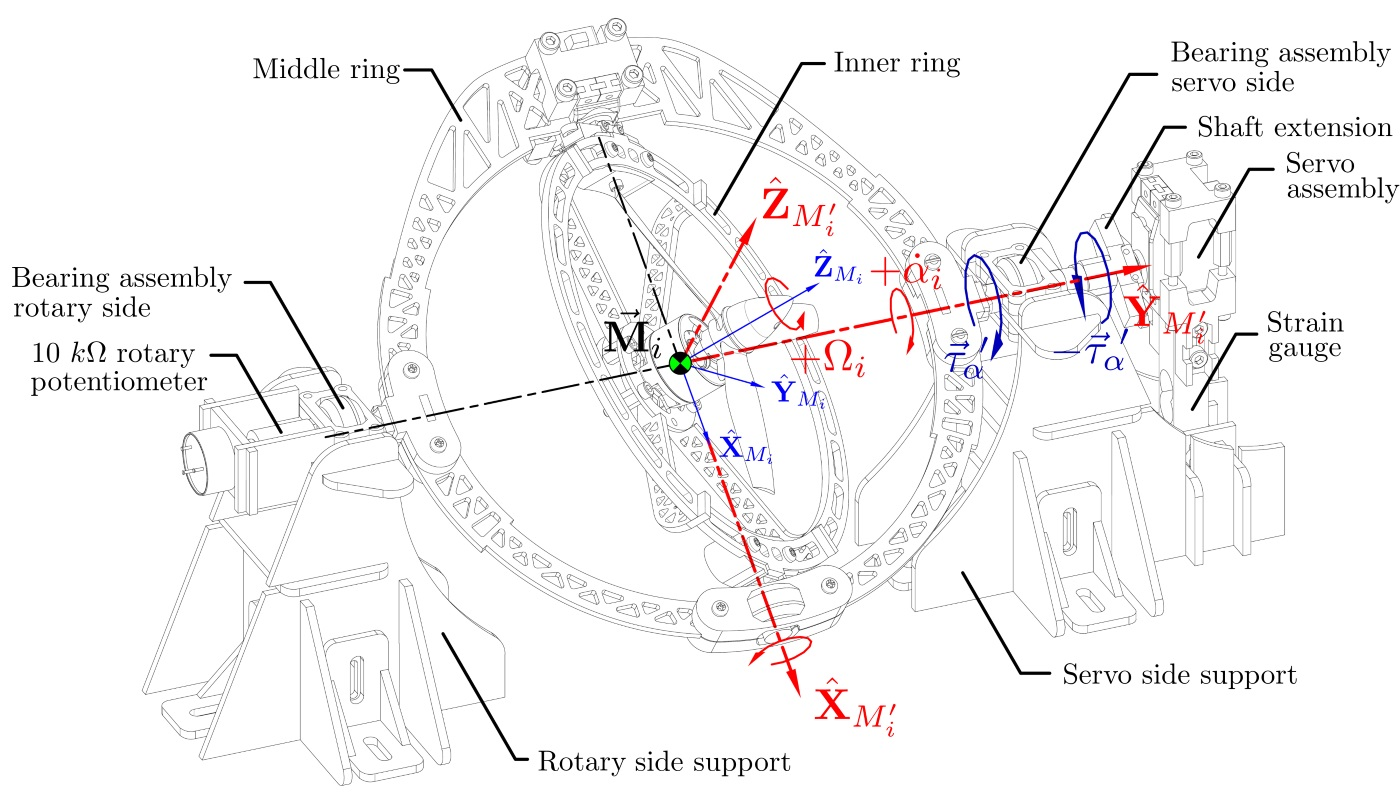
\includegraphics[width=0.9\textwidth]{figs/torque-middle}
\caption{Middle ring torque test rig}
\label{fig:torque-middle}
\vspace{-6pt}
\end{figure}
Similarly the middle ring test structure (Fig:\ref{fig:torque-middle}) contains inner and middle ring assemblies representing the entire motor module. The inner ring servo $\lambda_i$ is held at constant values to represent varying inertias for the net module $J_\text{p}$ described in Eq:\ref{eq:inertia.middle.b}. The outer servo $\alpha_i$ applies an accelerating torque $\vec{\tau}_\alpha$ with an opposing $-\vec{\tau}_\lambda$ response. Only the $\hat{Y}_{M_i'}$ component deflects the strain gauge and as such the torque measured by the strain gauge is:
\begin{equation}
\vec{\tau}_\alpha\text{}\hspace{-2pt}'(\lambda)=\vec{\tau}_\alpha(\lambda)\cdot\hat{Y}_{M_i'}~~~~\in\mathcal{F}^{M_i'}
\end{equation}
Reiterating the equation for the expected simulated torque $\hat{\tau}_\alpha(\lambda)$ from Eq:\ref{eq:torque-induced-middle} with an included gravitational component and induced torque as a result of the inner ring's rotation:
\begin{multline} \label{eq:model-middle}
\hat{\tau}_\alpha(\lambda_i)=R_x(\lambda)\vec{\tau}_\lambda+\big(\dot{J}_p'\big)\dot{\vec{\alpha}}_i+\Big(\dot{J}_n''-R_y(\alpha)\big(\dot{J}_n'\big)R_y^{-1}(\alpha)\Big)\dot{\vec{\lambda}}_i'+\Big(\dot{J}_r''-R_y(\alpha)\big(\dot{J}_r'\big)R_y^{-1}(\alpha)\Big)\vec{\Omega}_i''
\\
+\big(J_\text{p}'\big)\ddot{\vec{\alpha}}_i+\dot{\vec{\alpha}}_i\times \Big(\big(J_p'\big)\dot{\vec{\alpha}}_i+\big(J_n''\big)\dot{\vec{\lambda}}_i\hspace{-2pt}'+\big(J_r''\big)\vec{\Omega}_i\hspace{-2pt}''\Big)+m_\text{p}C.M'_{\text{p}}\times\vec{G}_{M_i}~~~~\in\mathcal{F}^{M_i''}
\end{multline}
Where the term $C.M_{\text{p}}''$ is the net rotated center of gravity for the entire motor module:
\begin{equation}
C.M_\text{p}'=\frac{m_\text{n}R_y(\alpha)R_x(\lambda)C.M_\text{n}+m_\text{m}R_y(\alpha)C.M_\text{m}}{m_\text{n}+m_\text{n}}
\end{equation}
Moreover, the included torque term $\hat{\tau}_\lambda$ is going to be zero for the case where the propeller's rotational speed and the inner ring's servo speed are both constant; $\dot{\vec{\Omega}}_i=0$ and $\dot{\vec{lambda}}_i=0$. Plotted in Fig:\ref{fig:tau-alpha} shows results for measured torques $\vec{\tau}_\alpha\text{}\hspace{-2pt}'(\lambda)$, expected simulated torque values $\hat{\tau}_\alpha(\lambda)$ and resultant SimScape simulation values for $\tilde{\tau}_\alpha(\lambda)$. Tests are conducted with a constant propeller rotational velocity $\vec{\Omega}_i=6500~~[\text{RPM}]$ but differing rotational positions for the inner ring servo $\lambda_i$. That angular position affects the net encountered rotational inertial $J_\text{p}(\lambda)$.
\begin{figure}[htbp]
\centering
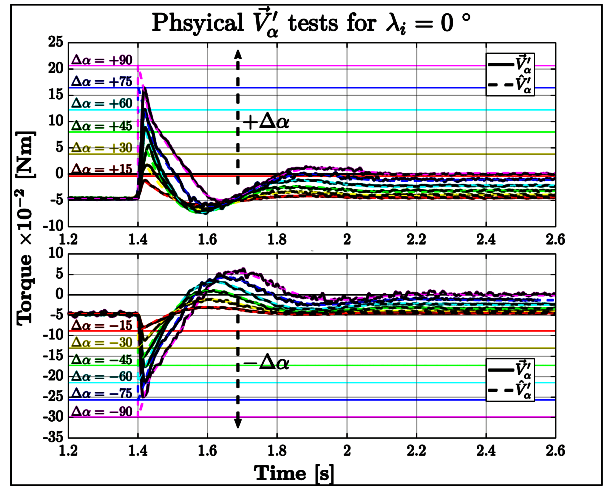
\includegraphics[width=0.55\textwidth]{graphs/tau-alpha}
\caption{Tests for $\vec{\tau}_\lambda$}
\label{fig:tau-alpha}
\end{figure}
\par
The final simulated module is that of $\hat{\tau}_b$
\par
\emph{\color{Gray}The above responses are pertinent to simulation and plant dependent feedback compensation. The simulation environment is structured such that the torques are produced as responses from Newtonian movement at every step interval. In due course it would be more efficient (and less stiff) for the simulation to exploit an implicit Euler\cite{physicallybased,multibodydynamics} coordinate system in lieu of the cartesian response equations developed above. However this was not implemented in Chapter:\ref{ch:simulation} and remains open to further testing and simulation\ldots}
%====================================================
\section{Consolidated Model}
\label{sec:dynamics.model}
%====================================================
Reiterating the different aspects detailed above and consolidating the state equations from Eq:\ref{eq:states.a}-\ref{eq:states.d}. Then lifting the attitude states to $\mathbb{R}^4$ space with the use of quaternions. Also introducing the non-linear inertial and gyroscopic responses to induced perturbations, $\vec{\tau}_\lambda$ and $\vec{\tau}_\alpha$ from Eq:\ref{eq:torque-induced-inner} and Eq:\ref{eq:torque-induced-middle} respectively, with non-linear inertial matrix terms $J_b(u)$ from Section:\ref{sec:proto.inertia}. Finally replacing net \emph{virtual} plant inputs, $\vec{\tau}_\mu$ and $\vec{F}_\mu$, with higher fidelity thrust models. The exact effectiveness actuator relationships are explored in Section:\ref{sec:control.inputs}. The following are state differential equations then used for subsequent control system development and simulation\ldots
\\
\begin{subequations}\label{eq:quaternion-states}
\begin{equation}\label{eq:quaternion-states-velocity}
\dot{\mathcal{E}}=Q_b^*\otimes\vec{v}_b\otimes Q_b~~~~\in\mathcal{F}^I
\end{equation}
\vspace{-10pt}
\begin{equation}\label{eq:quaternion-states-acceleration}
\dot{\vec{v}}_b=m^{-1}\big(-\vec{\omega}_b\times m\vec{v}_b+Q_b\otimes m\vec{G}_I\otimes Q_b^*-\vec{D}_{net}(\vec{v}_b)+\vec{F}_\mu(u)\big)~~~~\in\mathcal{F}^b
\end{equation}
\vspace{-8pt}
\begin{equation}\label{eq:quaternion-states-quaternion}
\dot{Q}_b=\frac{1}{2}Q_b\otimes \vec{\omega}_b ~~~~\in\mathcal{F}^I
\end{equation}
\vspace{-8pt}
\begin{equation}\label{eq:quaternion-states-angular}
\dot{\vec{\omega}}_b=\mathbb{I}_b(u)^{-1}\big(-\vec{\omega}_b \times \mathbb{I}_b(u)\vec{\omega}_b-\vec{\tau}_Q(u)+\vec{\tau}_g(u)+\sum_{i=1}^4 \vec{Q}(\Omega,\lambda,\alpha)+\mu\vec{\tau}(u)\big)~~~~\in\mathcal{F}^b
\end{equation}
\vspace{-10pt}
\begin{equation}
u=\big[\Omega_1^+,~\lambda_1,~\alpha_1,~\ldots~\Omega_4^-,~\lambda_4,~\alpha_4 \big]~~~~\in\mathbb{U}\in\mathbb{R}^{12}
\end{equation}
\end{subequations}
With net force and torque control plant inputs, $\vec{F}_\mu$ and $\vec{\tau}_\mu$ respectively. Both are later abstracted to virtual control inputs next in Ch:\ref{ch:control}, motor number subscripts $i\in[1:4]$ are implied in the following.
\begin{subequations}\label{eq:quaternion-inputs}
\begin{equation}
\vec{F}_\mu(u)=\sum_{i=1}^4 \vec{T}(\Omega,\lambda,\alpha)=\sum_{i=1}^4 Q_{M_i}^*\otimes T(\Omega)\otimes Q_{M_i}~~~~\in\mathcal{F}^b
\end{equation}
\vspace{-6pt}
\begin{equation}
\vec{\tau}_\mu(u)=\sum_{i=1}^4 \vec{l}\times\vec{T}(\Omega,\lambda,\alpha)=\sum_{i=1}^4 \vec{l}\times\big(Q_{M_i}^*\otimes T(\Omega)\otimes Q_{M_i}\big)~~~~\in\mathcal{F}^b
\end{equation}
\end{subequations}
Scalar thrust $T(\Omega)$ is a function of the propeller's rotational velocity whereas $\vec{T}(\Omega,\lambda,\alpha)$ is a vector in $\mathbb{R}^3$. The thrust vector is redirected similarly to Eq:\ref{eq:motor-module-rotation.a} and transformed to the frame $\mathcal{F}^b$. Equivalently $Q(\Omega)$ is the scalar aerodynamic torque in $\mathcal{F}^{M_i}$ about each motor's rotor $\hat{Z}$-axis, $\vec{Q}(\Omega,\lambda,\alpha)$ is the torque vector counterpart in $\mathcal{F}^b$. Both thrust and aerodynamic propeller torque terms are calculated from their respective coefficients (plotted in Fig:\ref{fig:coeffs-plot}):
\begin{subequations}
\begin{equation}\label{eq:aerodynamic-thrust}
T(\Omega)= C_T(J)\rho\Omega^2D^4~~~~[\text{N}]
\end{equation}
\vspace{-15pt}
\begin{equation}\label{eq:aerodynamic-torque}
Q(\Omega)= C_P(J)\rho\Omega^3D^5 \big(1/R\Omega\big)~~~~[\text{Nm}]
\end{equation}
\end{subequations}
Noting that $\Omega$ for aerodynamic calculations in Eq:\ref{eq:aerodynamic-thrust} and Eq:\ref{eq:aerodynamic-torque} has units $[\text{RPS}]$. Inertial torque responses from actuator input rates from Eq:\ref{eq:torque-response} are introduced as feedback compensation terms;
\begin{equation}\label{eq:actuator-torque}
\tau_Q(u)=\sum_{i=1}^4 -Q_{M_i}\otimes \tau_{\lambda_i}(u)\otimes Q_{M_i}^*-Q_{M_i'}\otimes \tau_{\alpha_i}(u) \otimes Q_{M_i'}^*~~~\in\mathcal{F}^b
\end{equation}
Then including variable gravitational torque arm from Eq:\ref{eq:grav-torque}, dependent on net actuator positions $u$:
\begin{equation}\label{eq:consolidated-grav-torque}
\vec{\tau}_g(u)=\Delta C.G \times\vec{G}_b~~~~\in\mathcal{F}^b
\end{equation}
And finally, the entire vehicles instantaneous inertia, taken from Eq:\ref{eq:body-net}, is given as:
\begin{equation}
\underset{u\in\mathbb{U}}{J_b(u)}=\underset{\vec{\mathbf{O}}_b}{J_{y}'}+\sum_{i=1}^{4} \underset{\vec{\mathbf{O}}_b}{J_{n}}+\sum_{i=1}^{4} \underset{\vec{\mathbf{O}}_b}{J_{m}}
\end{equation}
It is possible to bundle both attitude states (either euler angles $\vec{\eta}$ or quaternions $Q_b$) together with the linear translational position $\vec{\mathcal{E}}$ into a single state $\vec{\mathbf{x}}$. Which then has its own combined control law. This could potentially exploit the cross-product coupling terms between angular and linear displacements for control benefits.